% Options for packages loaded elsewhere
\PassOptionsToPackage{unicode}{hyperref}
\PassOptionsToPackage{hyphens}{url}
%
\documentclass[
]{article}
\usepackage{amsmath,amssymb}
\usepackage{lmodern}
\usepackage{ifxetex,ifluatex}
\ifnum 0\ifxetex 1\fi\ifluatex 1\fi=0 % if pdftex
  \usepackage[T1]{fontenc}
  \usepackage[utf8]{inputenc}
  \usepackage{textcomp} % provide euro and other symbols
\else % if luatex or xetex
  \usepackage{unicode-math}
  \defaultfontfeatures{Scale=MatchLowercase}
  \defaultfontfeatures[\rmfamily]{Ligatures=TeX,Scale=1}
\fi
% Use upquote if available, for straight quotes in verbatim environments
\IfFileExists{upquote.sty}{\usepackage{upquote}}{}
\IfFileExists{microtype.sty}{% use microtype if available
  \usepackage[]{microtype}
  \UseMicrotypeSet[protrusion]{basicmath} % disable protrusion for tt fonts
}{}
\makeatletter
\@ifundefined{KOMAClassName}{% if non-KOMA class
  \IfFileExists{parskip.sty}{%
    \usepackage{parskip}
  }{% else
    \setlength{\parindent}{0pt}
    \setlength{\parskip}{6pt plus 2pt minus 1pt}}
}{% if KOMA class
  \KOMAoptions{parskip=half}}
\makeatother
\usepackage{xcolor}
\IfFileExists{xurl.sty}{\usepackage{xurl}}{} % add URL line breaks if available
\IfFileExists{bookmark.sty}{\usepackage{bookmark}}{\usepackage{hyperref}}
\hypersetup{
  pdftitle={Assignments},
  hidelinks,
  pdfcreator={LaTeX via pandoc}}
\urlstyle{same} % disable monospaced font for URLs
\usepackage[margin=1in]{geometry}
\usepackage{color}
\usepackage{fancyvrb}
\newcommand{\VerbBar}{|}
\newcommand{\VERB}{\Verb[commandchars=\\\{\}]}
\DefineVerbatimEnvironment{Highlighting}{Verbatim}{commandchars=\\\{\}}
% Add ',fontsize=\small' for more characters per line
\usepackage{framed}
\definecolor{shadecolor}{RGB}{248,248,248}
\newenvironment{Shaded}{\begin{snugshade}}{\end{snugshade}}
\newcommand{\AlertTok}[1]{\textcolor[rgb]{0.94,0.16,0.16}{#1}}
\newcommand{\AnnotationTok}[1]{\textcolor[rgb]{0.56,0.35,0.01}{\textbf{\textit{#1}}}}
\newcommand{\AttributeTok}[1]{\textcolor[rgb]{0.77,0.63,0.00}{#1}}
\newcommand{\BaseNTok}[1]{\textcolor[rgb]{0.00,0.00,0.81}{#1}}
\newcommand{\BuiltInTok}[1]{#1}
\newcommand{\CharTok}[1]{\textcolor[rgb]{0.31,0.60,0.02}{#1}}
\newcommand{\CommentTok}[1]{\textcolor[rgb]{0.56,0.35,0.01}{\textit{#1}}}
\newcommand{\CommentVarTok}[1]{\textcolor[rgb]{0.56,0.35,0.01}{\textbf{\textit{#1}}}}
\newcommand{\ConstantTok}[1]{\textcolor[rgb]{0.00,0.00,0.00}{#1}}
\newcommand{\ControlFlowTok}[1]{\textcolor[rgb]{0.13,0.29,0.53}{\textbf{#1}}}
\newcommand{\DataTypeTok}[1]{\textcolor[rgb]{0.13,0.29,0.53}{#1}}
\newcommand{\DecValTok}[1]{\textcolor[rgb]{0.00,0.00,0.81}{#1}}
\newcommand{\DocumentationTok}[1]{\textcolor[rgb]{0.56,0.35,0.01}{\textbf{\textit{#1}}}}
\newcommand{\ErrorTok}[1]{\textcolor[rgb]{0.64,0.00,0.00}{\textbf{#1}}}
\newcommand{\ExtensionTok}[1]{#1}
\newcommand{\FloatTok}[1]{\textcolor[rgb]{0.00,0.00,0.81}{#1}}
\newcommand{\FunctionTok}[1]{\textcolor[rgb]{0.00,0.00,0.00}{#1}}
\newcommand{\ImportTok}[1]{#1}
\newcommand{\InformationTok}[1]{\textcolor[rgb]{0.56,0.35,0.01}{\textbf{\textit{#1}}}}
\newcommand{\KeywordTok}[1]{\textcolor[rgb]{0.13,0.29,0.53}{\textbf{#1}}}
\newcommand{\NormalTok}[1]{#1}
\newcommand{\OperatorTok}[1]{\textcolor[rgb]{0.81,0.36,0.00}{\textbf{#1}}}
\newcommand{\OtherTok}[1]{\textcolor[rgb]{0.56,0.35,0.01}{#1}}
\newcommand{\PreprocessorTok}[1]{\textcolor[rgb]{0.56,0.35,0.01}{\textit{#1}}}
\newcommand{\RegionMarkerTok}[1]{#1}
\newcommand{\SpecialCharTok}[1]{\textcolor[rgb]{0.00,0.00,0.00}{#1}}
\newcommand{\SpecialStringTok}[1]{\textcolor[rgb]{0.31,0.60,0.02}{#1}}
\newcommand{\StringTok}[1]{\textcolor[rgb]{0.31,0.60,0.02}{#1}}
\newcommand{\VariableTok}[1]{\textcolor[rgb]{0.00,0.00,0.00}{#1}}
\newcommand{\VerbatimStringTok}[1]{\textcolor[rgb]{0.31,0.60,0.02}{#1}}
\newcommand{\WarningTok}[1]{\textcolor[rgb]{0.56,0.35,0.01}{\textbf{\textit{#1}}}}
\usepackage{graphicx}
\makeatletter
\def\maxwidth{\ifdim\Gin@nat@width>\linewidth\linewidth\else\Gin@nat@width\fi}
\def\maxheight{\ifdim\Gin@nat@height>\textheight\textheight\else\Gin@nat@height\fi}
\makeatother
% Scale images if necessary, so that they will not overflow the page
% margins by default, and it is still possible to overwrite the defaults
% using explicit options in \includegraphics[width, height, ...]{}
\setkeys{Gin}{width=\maxwidth,height=\maxheight,keepaspectratio}
% Set default figure placement to htbp
\makeatletter
\def\fps@figure{htbp}
\makeatother
\setlength{\emergencystretch}{3em} % prevent overfull lines
\providecommand{\tightlist}{%
  \setlength{\itemsep}{0pt}\setlength{\parskip}{0pt}}
\setcounter{secnumdepth}{-\maxdimen} % remove section numbering
\ifluatex
  \usepackage{selnolig}  % disable illegal ligatures
\fi

\title{Assignments}
\author{}
\date{\vspace{-2.5em}}

\begin{document}
\maketitle

This page will contain all the assignments you submit for the class.

\hypertarget{instructions-for-all-assignments}{%
\subsubsection{Instructions for all
assignments}\label{instructions-for-all-assignments}}

I want you to submit your assignment as a PDF, so I can keep a record of
what the code looked like that day. I also want you to include your
answers on your personal GitHub website. This will be good practice for
editing your website and it will help you produce something you can keep
after the class is over.

\begin{enumerate}
\def\labelenumi{\arabic{enumi}.}
\item
  Download the Assignment1.Rmd file from Canvas. You can use this as a
  template for writing your answers. It's the same as what you can see
  on my website in the Assignments tab. Once we're done with this I'll
  edit the text on the website to include the solutions.
\item
  On RStudio, open a new R script in RStudio (File \textgreater{} New
  File \textgreater{} R Script). This is where you can test out your R
  code. You'll write your R commands and draw plots here.
\item
  Once you have finalized your code, copy and paste your results into
  this template (Assignment 1.Rmd). For example, if you produced a plot
  as the solution to one of the problems, you can copy and paste the R
  code in R markdown by using the
  \texttt{\textasciigrave{}\textasciigrave{}\{r\}\ \textasciigrave{}\textasciigrave{}\textasciigrave{}}
  command. Answer the questions in full sentences and Save.
\item
  Produce a PDF file with your answers. To do this, knit to PDF (use
  Knit button at the top of RStudio), locate the PDF file in your docs
  folder (it's in the same folder as the Rproj), and submit that on on
  Canvas in Assignment 1.
\item
  Build Website, go to GitHub desktop, commit and push. Now your
  solutions should be on your website as well.
\end{enumerate}

\hypertarget{assignment-1}{%
\section{Assignment 1}\label{assignment-1}}

\textbf{Collaborators: Lorem Ipsum. }

This assignment is due on Canvas on Monday 9/20 before class, at 10:15
am. Include the name of anyone with whom you collaborated at the top of
the assignment.

\hypertarget{problem-1}{%
\subsubsection{Problem 1}\label{problem-1}}

Install the datasets package on the console below using
\texttt{install.packages("datasets")}. Now load the library.

\begin{Shaded}
\begin{Highlighting}[]
\FunctionTok{options}\NormalTok{(}\AttributeTok{repos =} \FunctionTok{list}\NormalTok{(}\AttributeTok{CRAN=}\StringTok{"http://cran.rstudio.com/"}\NormalTok{))}
\CommentTok{\#install.packages ("dataset\_load")}
\end{Highlighting}
\end{Shaded}

Load the USArrests dataset and rename it \texttt{dat}. Note that this
dataset comes with R, in the package datasets, so there's no need to
load data from your computer. Why is it useful to rename the dataset?

\begin{Shaded}
\begin{Highlighting}[]
\NormalTok{dat }\OtherTok{\textless{}{-}}\NormalTok{ USArrests}
\end{Highlighting}
\end{Shaded}

Answer: It is useful to rename datasets because it is good practice and
it is more convenient to use instead of the full names of data sets
which are usually longer. Also, might reduce errors in using a short and
simple name such as dat.

\hypertarget{problem-2}{%
\subsubsection{Problem 2}\label{problem-2}}

Use this command to make the state names into a new variable called
State.

\begin{Shaded}
\begin{Highlighting}[]
\NormalTok{dat}\SpecialCharTok{$}\NormalTok{state }\OtherTok{\textless{}{-}} \FunctionTok{tolower}\NormalTok{(}\FunctionTok{rownames}\NormalTok{(USArrests))}
\end{Highlighting}
\end{Shaded}

This dataset has the state names as row names, so we just want to make
them into a new variable. We also make them all lower case, because that
will help us draw a map later - the map function requires the states to
be lower case.

List the variables contained in the dataset \texttt{USArrests}.

\begin{Shaded}
\begin{Highlighting}[]
\FunctionTok{names}\NormalTok{(dat)}
\end{Highlighting}
\end{Shaded}

\begin{verbatim}
## [1] "Murder"   "Assault"  "UrbanPop" "Rape"     "state"
\end{verbatim}

The five variables are Murder, Assault, UrbanPop, Rape, and State.

\hypertarget{problem-3}{%
\subsubsection{Problem 3}\label{problem-3}}

What type of variable (from the DVB chapter) is \texttt{Murder}?

Answer: Murder is a quantitative variable.

What R Type of variable is it?

\begin{Shaded}
\begin{Highlighting}[]
\FunctionTok{class}\NormalTok{(dat}\SpecialCharTok{$}\NormalTok{Murder)}
\end{Highlighting}
\end{Shaded}

\begin{verbatim}
## [1] "numeric"
\end{verbatim}

Answer: Murder is a numeric value.

\hypertarget{problem-4}{%
\subsubsection{Problem 4}\label{problem-4}}

What information is contained in this dataset, in general? What do the
numbers mean?

Answer: This dataset includes the number of murder, assault, urbanpop,
and rape cases throughout 50 states. The datasets relies on the recorded
cases of crimes that offenders/criminals commit. It was most likely
collected from the series of reported crime statisitcs on the internet
or perhaps even the Federal Bureau of Justice Statistics. The numbers
represent the frequency of that crime for each state. I assume that
reserchers of crime rates,statiticians in the field of law enforcement
or legal justice created this dataset to compare crime rates across the
U.S. but also the frequency of the different crimes against each other.

\hypertarget{problem-5}{%
\subsubsection{Problem 5}\label{problem-5}}

Draw a histogram of \texttt{Murder} with proper labels and title.

\begin{Shaded}
\begin{Highlighting}[]
\FunctionTok{hist}\NormalTok{(dat}\SpecialCharTok{$}\NormalTok{Murder, }\AttributeTok{main=}\StringTok{"Histogram of Murder"}\NormalTok{, }\AttributeTok{xlab=}\StringTok{"Arrests per 100,000 Residents"}\NormalTok{, }\AttributeTok{ylab=}\StringTok{"Frequency"}\NormalTok{)}
\end{Highlighting}
\end{Shaded}

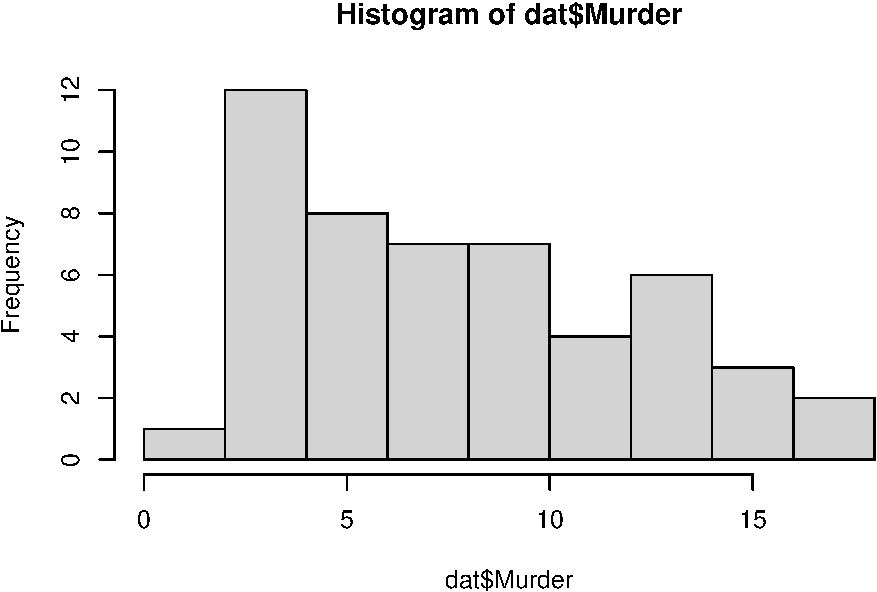
\includegraphics{Assignments_files/figure-latex/unnamed-chunk-6-1.pdf}

\hypertarget{problem-6}{%
\subsubsection{Problem 6}\label{problem-6}}

Please summarize \texttt{Murder} quantitatively. What are its mean and
median? What is the difference between mean and median? What is a
quartile, and why do you think R gives you the 1st Qu. and 3rd Qu.?

\begin{Shaded}
\begin{Highlighting}[]
\FunctionTok{summary}\NormalTok{(dat}\SpecialCharTok{$}\NormalTok{Murder)}
\end{Highlighting}
\end{Shaded}

\begin{verbatim}
##    Min. 1st Qu.  Median    Mean 3rd Qu.    Max. 
##   0.800   4.075   7.250   7.788  11.250  17.400
\end{verbatim}

The mean is 7.788 and the median is 7.250. Mean is the average of the
data set. It is found by adding all the numbers in the data set and then
dividing by the number of values in the set. The median is the middle
value when a data set is ordered from least to greatest. A quartile is a
type of quantile which divides the data set into four parts. You can
deduce the interquartile range (IQR) from Q1 and Q3 and this is
significant because the IQR, also known as the midspread/middle 50\%/H
spread is a measure of statistical dispersion or the variability in a
data set.

\hypertarget{problem-7-a}{%
\subsubsection{Problem 7 (a)}\label{problem-7-a}}

Repeat the same steps you followed for \texttt{Murder}, for the
variables \texttt{Assault} and \texttt{Rape}.

\begin{Shaded}
\begin{Highlighting}[]
\FunctionTok{hist}\NormalTok{(dat}\SpecialCharTok{$}\NormalTok{Assault, }\AttributeTok{main=}\StringTok{"Histogram of Assault"}\NormalTok{, }\AttributeTok{xlab=}\StringTok{"Arrests per 100,000 Residents"}\NormalTok{, }\AttributeTok{ylab=}\StringTok{"Frequency"}\NormalTok{)}
\end{Highlighting}
\end{Shaded}

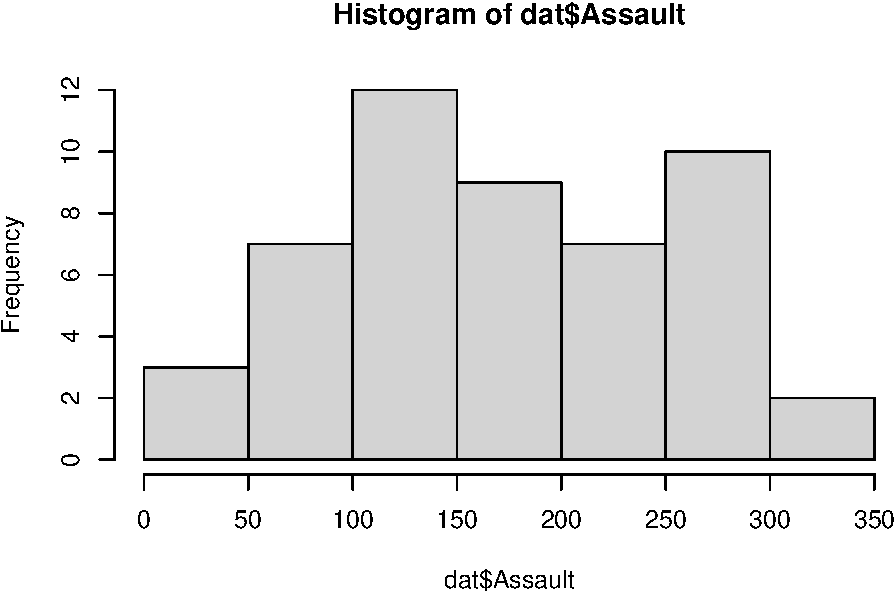
\includegraphics{Assignments_files/figure-latex/unnamed-chunk-8-1.pdf}

\begin{Shaded}
\begin{Highlighting}[]
\FunctionTok{summary}\NormalTok{(dat}\SpecialCharTok{$}\NormalTok{Assault)}
\end{Highlighting}
\end{Shaded}

\begin{verbatim}
##    Min. 1st Qu.  Median    Mean 3rd Qu.    Max. 
##    45.0   109.0   159.0   170.8   249.0   337.0
\end{verbatim}

The mean is 170.8 and the median is 159.0.

\begin{Shaded}
\begin{Highlighting}[]
\FunctionTok{hist}\NormalTok{(dat}\SpecialCharTok{$}\NormalTok{Rape, }\AttributeTok{main=}\StringTok{"Histogram of Rape"}\NormalTok{, }\AttributeTok{xlab=}\StringTok{"Arrests per 100,000 Residents"}\NormalTok{, }\AttributeTok{ylab=}\StringTok{"Frequency"}\NormalTok{)}
\end{Highlighting}
\end{Shaded}

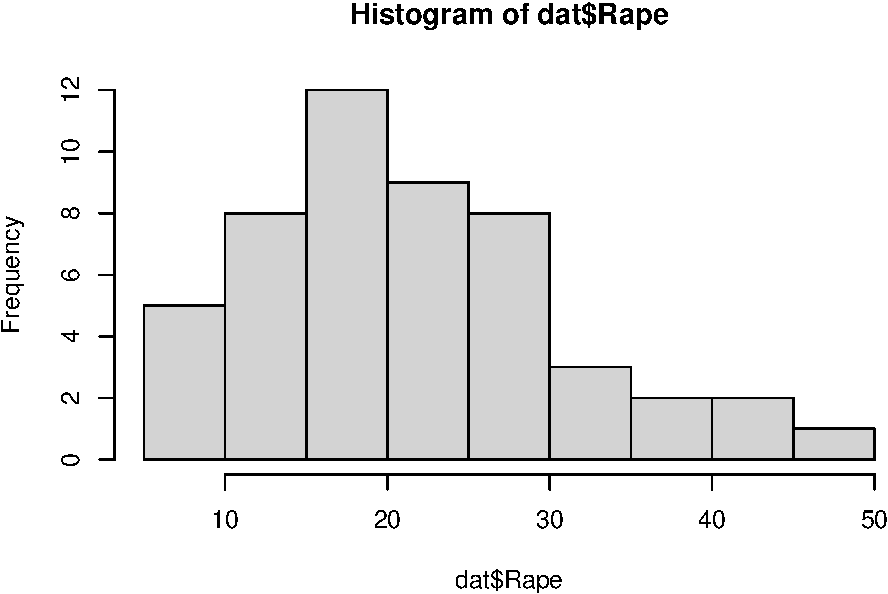
\includegraphics{Assignments_files/figure-latex/unnamed-chunk-10-1.pdf}

\begin{Shaded}
\begin{Highlighting}[]
\FunctionTok{summary}\NormalTok{(dat}\SpecialCharTok{$}\NormalTok{Rape)}
\end{Highlighting}
\end{Shaded}

\begin{verbatim}
##    Min. 1st Qu.  Median    Mean 3rd Qu.    Max. 
##    7.30   15.07   20.10   21.23   26.18   46.00
\end{verbatim}

The mean is 21.23 and the median is 20.10.

\hypertarget{problem-7-b}{%
\subsubsection{Problem 7 (b)}\label{problem-7-b}}

Now plot all three histograms together. You can do this by using the
command \texttt{par(mfrow=c(3,1))} and then plotting each of the three.

\begin{Shaded}
\begin{Highlighting}[]
\FunctionTok{par}\NormalTok{(}\AttributeTok{mfrow=}\FunctionTok{c}\NormalTok{(}\DecValTok{3}\NormalTok{,}\DecValTok{1}\NormalTok{))}
\FunctionTok{hist}\NormalTok{(dat}\SpecialCharTok{$}\NormalTok{Murder, }\AttributeTok{main=}\StringTok{"Histogram of Murder"}\NormalTok{, }\AttributeTok{xlab=}\StringTok{"Arrests per 100,000 Residents"}\NormalTok{, }\AttributeTok{ylab=}\StringTok{"Frequency"}\NormalTok{)}
\FunctionTok{hist}\NormalTok{(dat}\SpecialCharTok{$}\NormalTok{Assault, }\AttributeTok{main=}\StringTok{"Histogram of Assault"}\NormalTok{, }\AttributeTok{xlab=}\StringTok{"Arrests per 100,000 Residents"}\NormalTok{, }\AttributeTok{ylab=}\StringTok{"Frequency"}\NormalTok{)}
\FunctionTok{hist}\NormalTok{(dat}\SpecialCharTok{$}\NormalTok{Rape, }\AttributeTok{main=}\StringTok{"Histogram of Rape"}\NormalTok{, }\AttributeTok{xlab=}\StringTok{"Arrests per 100,000 Residents"}\NormalTok{, }\AttributeTok{ylab=}\StringTok{"Frequency"}\NormalTok{)}
\end{Highlighting}
\end{Shaded}

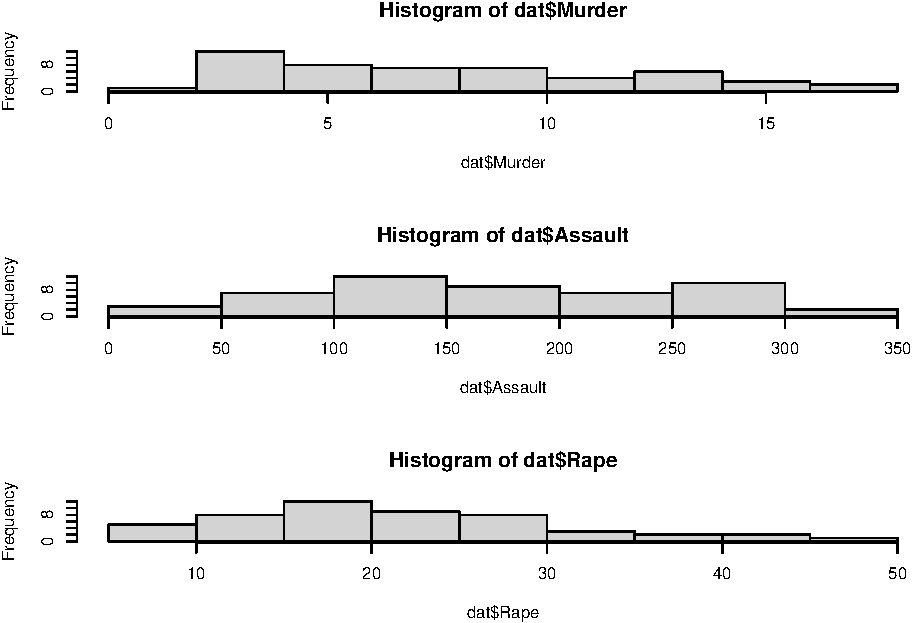
\includegraphics{Assignments_files/figure-latex/unnamed-chunk-12-1.pdf}

What does the command par do, in your own words (you can look this up by
asking R \texttt{?par})?

\begin{Shaded}
\begin{Highlighting}[]
\NormalTok{?par}
\end{Highlighting}
\end{Shaded}

Answer: par can be used to set either give you information about graphs
and/or let you set parameters for graphs.

What can you learn from plotting the histograms together?

Answer: By plotting the histogams together, we can observe the scale at
which the different crimes occurred. You can compare the frequencies
across the different crimes too.

Problem 8

In the console below (not in text), type
\texttt{install.packages("maps")} and press Enter, and then type
\texttt{install.packages("ggplot2")} and press Enter. This will install
the packages so you can load the libraries.

Run this code:

\begin{Shaded}
\begin{Highlighting}[]
\FunctionTok{install.packages}\NormalTok{(}\StringTok{"maps"}\NormalTok{)}
\FunctionTok{install.packages}\NormalTok{(}\StringTok{"ggplot2"}\NormalTok{)}

\FunctionTok{library}\NormalTok{(maps)}
\FunctionTok{library}\NormalTok{(ggplot2) }

\FunctionTok{ggplot}\NormalTok{(dat, }\FunctionTok{aes}\NormalTok{(}\AttributeTok{map\_id=}\NormalTok{state, }\AttributeTok{fill=}\NormalTok{Murder)) }\SpecialCharTok{+} 
  \FunctionTok{geom\_map}\NormalTok{(}\AttributeTok{map=}\FunctionTok{map\_data}\NormalTok{(}\StringTok{"state"}\NormalTok{)) }\SpecialCharTok{+} 
  \FunctionTok{expand\_limits}\NormalTok{(}\AttributeTok{x=}\FunctionTok{map\_data}\NormalTok{(}\StringTok{"state"}\NormalTok{)}\SpecialCharTok{$}\NormalTok{long, }\AttributeTok{y=}\FunctionTok{map\_data}\NormalTok{(}\StringTok{"state"}\NormalTok{)}\SpecialCharTok{$}\NormalTok{lat)}
\end{Highlighting}
\end{Shaded}

What does this code do? Explain what each line is doing.

Answer: The first line determines the dimensions of the graph. The
second and third line installs the package necessary to make the graph,
specifically a map. The fourth and fifth lines load the library of the
two packages necessary to construct a map. The sixth lines tells the map
to only include states and the frequency of Murder in each state. The
last three lines serves as the data frame that contains the map
coordinates.

\hypertarget{assignment-2}{%
\section{Assignment 2}\label{assignment-2}}

Problem 1: Load data

Set your working directory to the folder where you downloaded the data.

\begin{Shaded}
\begin{Highlighting}[]
\FunctionTok{setwd}\NormalTok{(}\StringTok{"/Users/isatounjie/Documents/GitHub/Aishas{-}Website/Assignment 2"}\NormalTok{)}
\end{Highlighting}
\end{Shaded}

Read the data

\begin{Shaded}
\begin{Highlighting}[]
\NormalTok{dat }\OtherTok{\textless{}{-}} \FunctionTok{read.csv}\NormalTok{(}\StringTok{"dat.nsduh.small.1.csv"}\NormalTok{)}
\end{Highlighting}
\end{Shaded}

What are the dimensions of the dataset?

\begin{Shaded}
\begin{Highlighting}[]
\FunctionTok{names}\NormalTok{(dat)}
\end{Highlighting}
\end{Shaded}

\begin{verbatim}
## [1] "mjage"     "cigage"    "iralcage"  "age2"      "sexatract" "speakengl"
## [7] "irsex"
\end{verbatim}

Answer: The dimensions of the dataset are mjage, cigage, iralcage, age2,
sexatract, speakengl, and irsex.

\hypertarget{problem-2-variables}{%
\subsection{Problem 2: Variables}\label{problem-2-variables}}

\begin{Shaded}
\begin{Highlighting}[]
\FunctionTok{class}\NormalTok{(dat}\SpecialCharTok{$}\NormalTok{mjage)}
\end{Highlighting}
\end{Shaded}

\begin{verbatim}
## [1] "integer"
\end{verbatim}

\begin{Shaded}
\begin{Highlighting}[]
\FunctionTok{class}\NormalTok{(dat}\SpecialCharTok{$}\NormalTok{cigage)}
\end{Highlighting}
\end{Shaded}

\begin{verbatim}
## [1] "integer"
\end{verbatim}

\begin{Shaded}
\begin{Highlighting}[]
\FunctionTok{class}\NormalTok{(dat}\SpecialCharTok{$}\NormalTok{iralcage)}
\end{Highlighting}
\end{Shaded}

\begin{verbatim}
## [1] "integer"
\end{verbatim}

\begin{Shaded}
\begin{Highlighting}[]
\FunctionTok{class}\NormalTok{(dat}\SpecialCharTok{$}\NormalTok{age2)}
\end{Highlighting}
\end{Shaded}

\begin{verbatim}
## [1] "integer"
\end{verbatim}

\begin{Shaded}
\begin{Highlighting}[]
\FunctionTok{class}\NormalTok{(dat}\SpecialCharTok{$}\NormalTok{sexatract)}
\end{Highlighting}
\end{Shaded}

\begin{verbatim}
## [1] "integer"
\end{verbatim}

\begin{Shaded}
\begin{Highlighting}[]
\FunctionTok{class}\NormalTok{(dat}\SpecialCharTok{$}\NormalTok{speakengl)}
\end{Highlighting}
\end{Shaded}

\begin{verbatim}
## [1] "integer"
\end{verbatim}

\begin{Shaded}
\begin{Highlighting}[]
\FunctionTok{class}\NormalTok{(dat}\SpecialCharTok{$}\NormalTok{irsex)}
\end{Highlighting}
\end{Shaded}

\begin{verbatim}
## [1] "integer"
\end{verbatim}

Describe the variables in the dataset.

Answer: It appears that mjage, cigage, iralcage, age2, sexatract, and
speakengl are all ordinal variables and irsex is a categorical variable.
It could also be regarded as an ordinal variable. In terms of r type,
they are all intergers.

What is this dataset about? Who collected the data, what kind of sample
is it, and what was the purpose of generating the data?

Answer: This dataset observes the age at which participants first tried
marijuana, first started smoking cigarettes every day,first tried
alcohol, what they identify as in terms of gender, their sexual
attraction, how well they speak English as well as the final recorded
age of the participants. The data was collected from The National Survey
on Drug Use and Health, specifically RTI International. Even though
participants are selected and then interviewed, I believe this is an
example of simple random sampling. Participants aren't chosen just
because they fit a certain criteria.

\hypertarget{problem-3-age-and-gender}{%
\subsection{Problem 3: Age and gender}\label{problem-3-age-and-gender}}

What is the age distribution of the sample like? Make sure you read the
codebook to know what the variable values mean.

Answer: Ranges 1-10 signify a participant at one, specific age, however
ranges 11-12 signify an option between two ages, and ranges 13-16
signify a range of ages. 17 signifies the largest range with
participants that are 65 or older.

Do you think this age distribution representative of the US population?
Why or why not?

Answer: Yes, I believe this is representative of the US population in
the context of this study. Children start experimenting (in terms of
drugs, sex, and alcohol) around the age of 12. Also, it is unlikely to
receive parental consent for a study like this for children that are too
young.

*Correction: They cut off the survey at age 12 by design, not because
they found people used drugs less below that age (although that is
probably also true). There are other surveys of children's use of drugs.

Is the sample balanced in terms of gender? If not, are there more
females or males?

\begin{Shaded}
\begin{Highlighting}[]
\FunctionTok{hist}\NormalTok{(dat}\SpecialCharTok{$}\NormalTok{irsex)}
\end{Highlighting}
\end{Shaded}

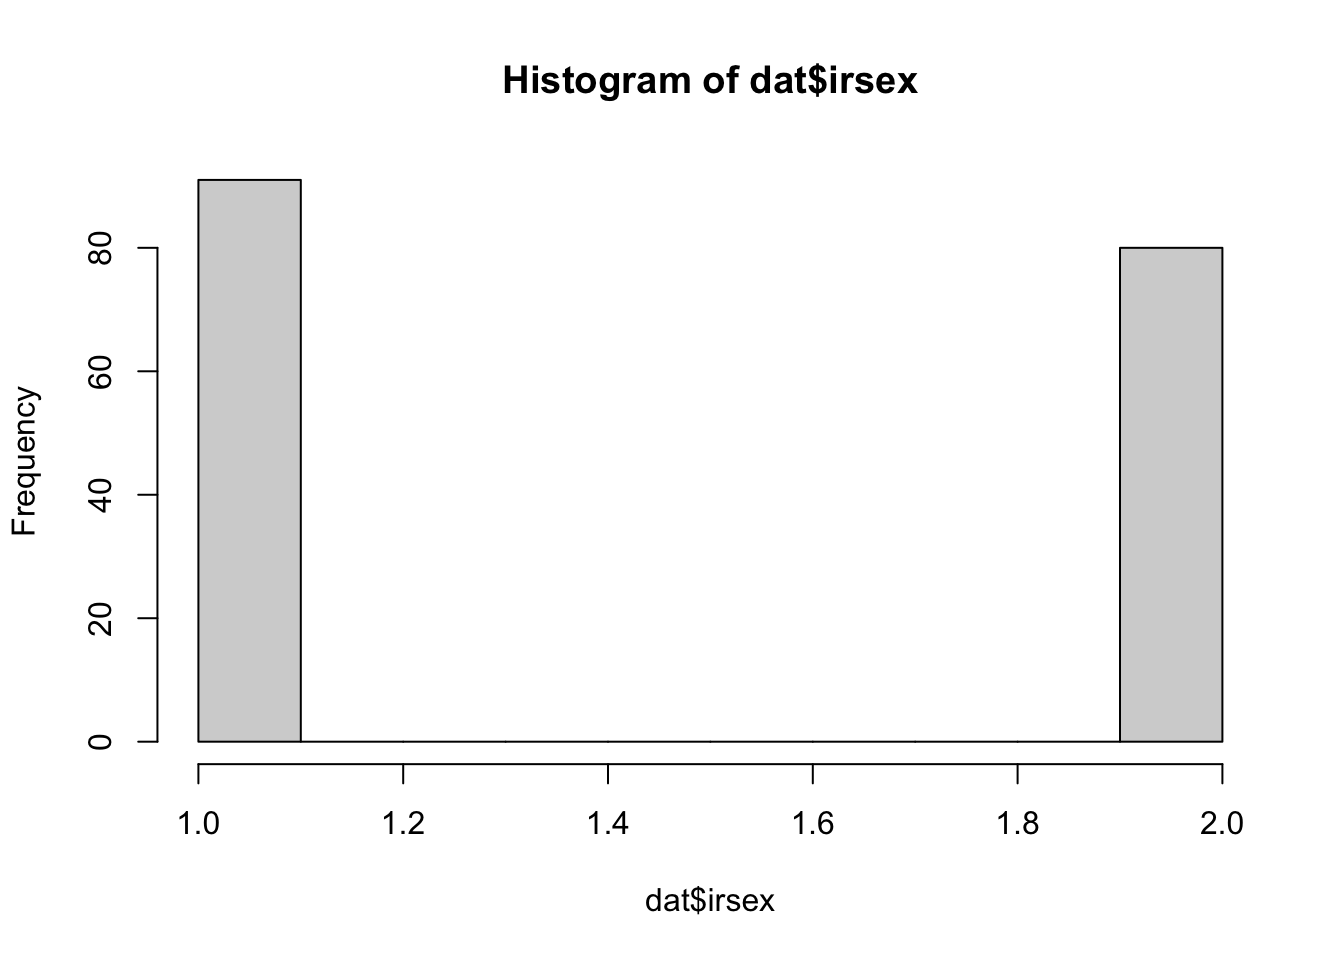
\includegraphics{Assignments_files/figure-latex/unnamed-chunk-19-1.pdf}

Answer: This sample is nearly balanced, there are 91 participants that
identify as male and 80 that identify as female.

Use this code to draw a stacked bar plot to view the relationship
between sex and age. What can you conclude from this plot?

\begin{Shaded}
\begin{Highlighting}[]
\FunctionTok{table}\NormalTok{(dat}\SpecialCharTok{$}\NormalTok{irsex,dat}\SpecialCharTok{$}\NormalTok{age2)}
\end{Highlighting}
\end{Shaded}

\begin{verbatim}
##    
##      4  6  7  8  9 10 11 12 13 14 15 16 17
##   1  1  1  1  0  1  1  3  3 14 10 33 14  9
##   2  1  0  0  2  6  2  3  4 13  6 29 10  4
\end{verbatim}

\begin{Shaded}
\begin{Highlighting}[]
\FunctionTok{head}\NormalTok{(dat)}
\end{Highlighting}
\end{Shaded}

\begin{verbatim}
##   mjage cigage iralcage age2 sexatract speakengl irsex
## 1    14     50       14   16         1         1     1
## 2    11     14        5   13         2         1     2
## 3    12     35       12   15         2         1     2
## 4    16     18       18   14         1         1     1
## 5    14     16       14   16         4         1     1
## 6    12     16       18   15         4         1     2
\end{verbatim}

\begin{Shaded}
\begin{Highlighting}[]
\NormalTok{tab.agesex }\OtherTok{\textless{}{-}} \FunctionTok{table}\NormalTok{(dat}\SpecialCharTok{$}\NormalTok{irsex,dat}\SpecialCharTok{$}\NormalTok{age2)}
\FunctionTok{barplot}\NormalTok{(tab.agesex,}
        \AttributeTok{main =} \StringTok{"Stacked barchart"}\NormalTok{,}
        \AttributeTok{xlab =} \StringTok{"Age category"}\NormalTok{, }\AttributeTok{ylab =} \StringTok{"Frequency"}\NormalTok{,}
        \AttributeTok{legend.text =} \FunctionTok{rownames}\NormalTok{(tab.agesex),}
        \AttributeTok{beside =} \ConstantTok{FALSE}\NormalTok{) }\CommentTok{\# Stacked bars (default)}
\end{Highlighting}
\end{Shaded}

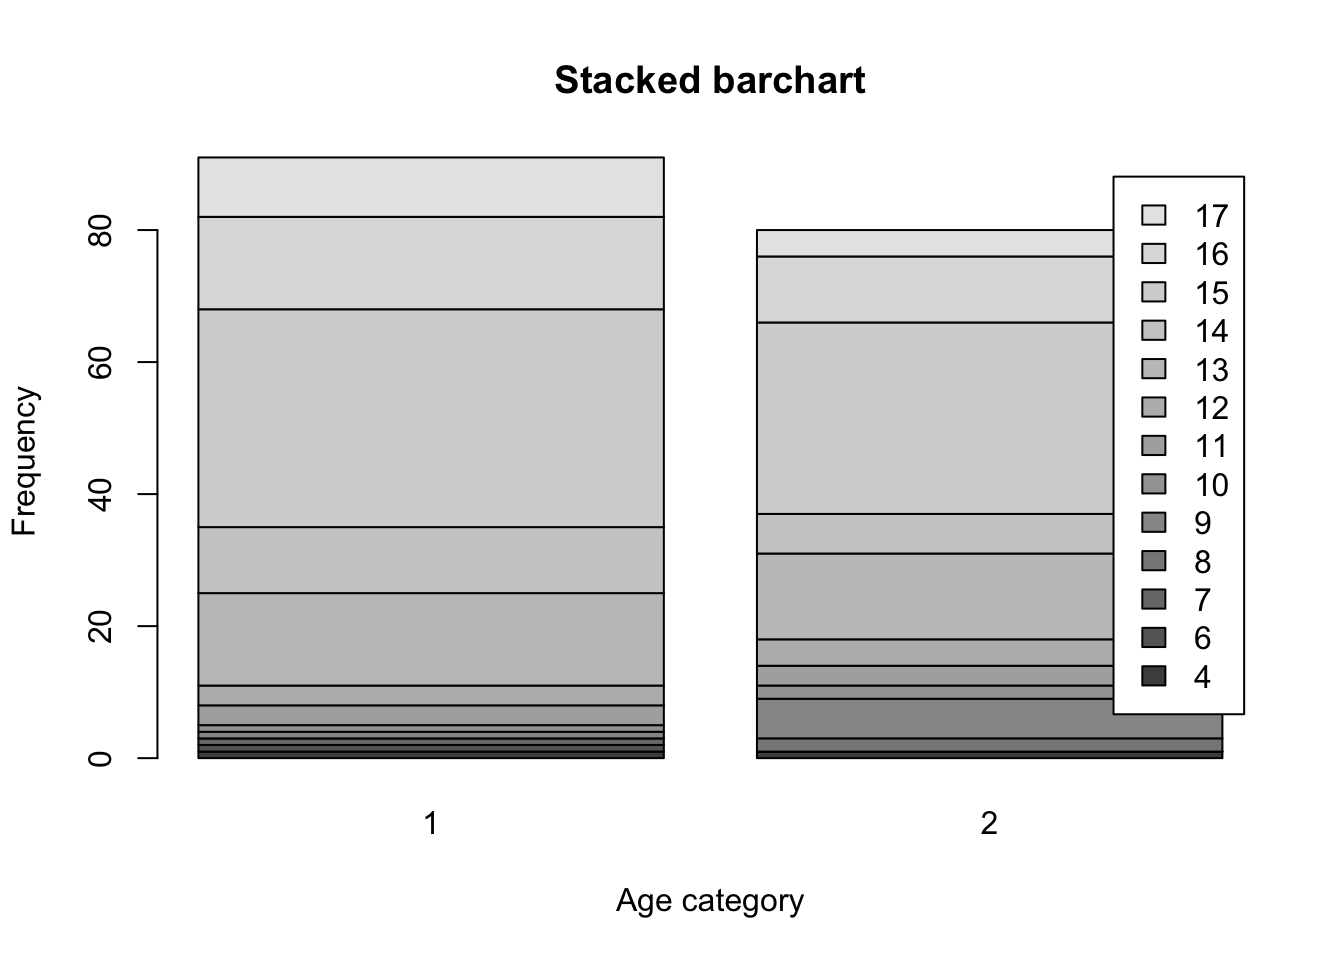
\includegraphics{Assignments_files/figure-latex/unnamed-chunk-20-1.pdf}

Answer: In the youngest age group (4) and group 11, there is an even
split. In age groups 6, 7, 13, 14, 15, 16, and 17 there are more men
than female, however in age groups 8, 9,10, and 12 there are more
females. Men dominate the majority of all the age groups.

\hypertarget{problem-4-substance-use}{%
\subsection{Problem 4: Substance use}\label{problem-4-substance-use}}

*correction: table is not needed. just look at lowest value for all the
different groups.

\emph{why do the age values go past 17 for mjage, cigage, and iralcage.
}barplots don't actually help to see this, but I don't know how to get a
breakdown of the data points within each group.

For which of the three substances included in the dataset (marijuana,
alcohol, and cigarettes) do individuals tend to use the substance
earlier?

Individuals tend to use alcohol earliest.

\begin{Shaded}
\begin{Highlighting}[]
\FunctionTok{table}\NormalTok{(dat}\SpecialCharTok{$}\NormalTok{mjage,dat}\SpecialCharTok{$}\NormalTok{age2)}
\end{Highlighting}
\end{Shaded}

\begin{verbatim}
##     
##      4 6 7 8 9 10 11 12 13 14 15 16 17
##   7  0 0 0 0 0  0  0  0  1  0  0  0  0
##   9  1 0 0 0 0  0  0  0  1  1  0  1  0
##   10 0 0 0 0 0  0  0  0  0  1  0  1  0
##   11 0 0 0 1 0  0  0  0  1  0  3  1  1
##   12 0 0 0 0 0  0  1  1  2  0  5  1  0
##   13 0 1 0 0 2  0  1  1  4  1  5  1  0
##   14 1 0 0 0 2  1  0  0  2  3  9  4  0
##   15 0 0 0 0 1  1  1  0  2  0  8  6  3
##   16 0 0 0 1 0  0  1  3  5  5  7  6  0
##   17 0 0 0 0 2  1  1  1  3  1  5  1  1
##   18 0 0 1 0 0  0  1  1  0  1  8  2  2
##   19 0 0 0 0 0  0  0  0  2  0  2  0  0
##   20 0 0 0 0 0  0  0  0  0  2  4  0  1
##   21 0 0 0 0 0  0  0  0  2  0  1  0  3
##   22 0 0 0 0 0  0  0  0  1  0  1  0  0
##   25 0 0 0 0 0  0  0  0  1  0  0  0  1
##   27 0 0 0 0 0  0  0  0  0  0  2  0  0
##   30 0 0 0 0 0  0  0  0  0  0  1  0  0
##   32 0 0 0 0 0  0  0  0  0  0  0  0  1
##   33 0 0 0 0 0  0  0  0  0  1  0  0  0
##   35 0 0 0 0 0  0  0  0  0  0  1  0  0
\end{verbatim}

\begin{Shaded}
\begin{Highlighting}[]
\FunctionTok{head}\NormalTok{(dat)}
\end{Highlighting}
\end{Shaded}

\begin{verbatim}
##   mjage cigage iralcage age2 sexatract speakengl irsex
## 1    14     50       14   16         1         1     1
## 2    11     14        5   13         2         1     2
## 3    12     35       12   15         2         1     2
## 4    16     18       18   14         1         1     1
## 5    14     16       14   16         4         1     1
## 6    12     16       18   15         4         1     2
\end{verbatim}

\begin{Shaded}
\begin{Highlighting}[]
\NormalTok{tab.agemjage }\OtherTok{\textless{}{-}} \FunctionTok{table}\NormalTok{(dat}\SpecialCharTok{$}\NormalTok{mjage,dat}\SpecialCharTok{$}\NormalTok{age2)}
\FunctionTok{barplot}\NormalTok{(tab.agemjage,}
        \AttributeTok{main =} \StringTok{"Stacked barchart"}\NormalTok{,}
        \AttributeTok{xlab =} \StringTok{"Age category"}\NormalTok{, }\AttributeTok{ylab =} \StringTok{"Frequency"}\NormalTok{,}
        \AttributeTok{legend.text =} \FunctionTok{rownames}\NormalTok{(tab.agemjage),}
        \AttributeTok{beside =} \ConstantTok{FALSE}\NormalTok{) }\CommentTok{\# Stacked bars (default)}
\end{Highlighting}
\end{Shaded}

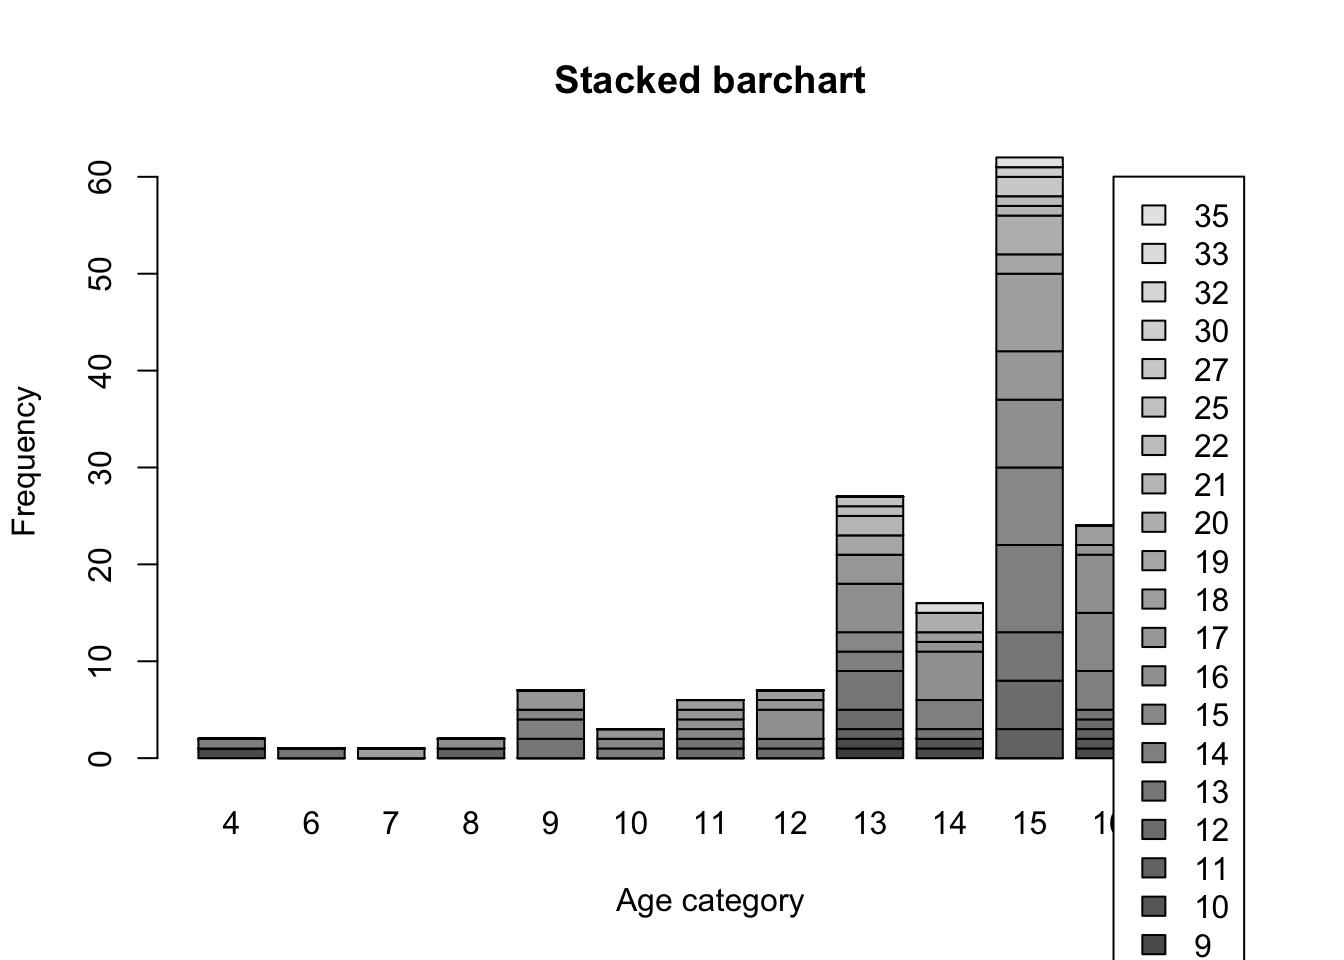
\includegraphics{Assignments_files/figure-latex/unnamed-chunk-21-1.pdf}

Earliest age range is 8.

\begin{Shaded}
\begin{Highlighting}[]
\FunctionTok{table}\NormalTok{(dat}\SpecialCharTok{$}\NormalTok{cigage,dat}\SpecialCharTok{$}\NormalTok{age2)}
\end{Highlighting}
\end{Shaded}

\begin{verbatim}
##     
##       4  6  7  8  9 10 11 12 13 14 15 16 17
##   10  0  0  0  0  0  0  0  0  0  0  1  0  0
##   11  0  0  0  0  0  0  0  0  0  0  0  0  1
##   12  0  0  0  0  0  0  0  1  1  0  0  1  0
##   13  1  0  0  0  0  0  0  0  0  0  5  3  1
##   14  1  0  1  0  1  0  0  1  2  0  3  1  0
##   15  0  1  0  0  2  0  1  0  6  0 10  4  1
##   16  0  0  0  0  0  1  1  0  4  3  8  7  1
##   17  0  0  0  2  2  1  0  1  4  3  2  2  3
##   18  0  0  0  0  2  1  3  2  4  4 12  2  1
##   19  0  0  0  0  0  0  0  2  2  1  6  0  0
##   20  0  0  0  0  0  0  1  0  2  0  4  2  1
##   21  0  0  0  0  0  0  0  0  1  1  4  0  0
##   22  0  0  0  0  0  0  0  0  0  1  3  0  1
##   23  0  0  0  0  0  0  0  0  0  2  1  1  0
##   24  0  0  0  0  0  0  0  0  1  0  0  0  0
##   25  0  0  0  0  0  0  0  0  0  1  1  0  2
##   27  0  0  0  0  0  0  0  0  0  0  1  0  0
##   35  0  0  0  0  0  0  0  0  0  0  1  0  0
##   45  0  0  0  0  0  0  0  0  0  0  0  0  1
##   50  0  0  0  0  0  0  0  0  0  0  0  1  0
\end{verbatim}

\begin{Shaded}
\begin{Highlighting}[]
\FunctionTok{head}\NormalTok{(dat)}
\end{Highlighting}
\end{Shaded}

\begin{verbatim}
##   mjage cigage iralcage age2 sexatract speakengl irsex
## 1    14     50       14   16         1         1     1
## 2    11     14        5   13         2         1     2
## 3    12     35       12   15         2         1     2
## 4    16     18       18   14         1         1     1
## 5    14     16       14   16         4         1     1
## 6    12     16       18   15         4         1     2
\end{verbatim}

\begin{Shaded}
\begin{Highlighting}[]
\NormalTok{tab.agecigage }\OtherTok{\textless{}{-}} \FunctionTok{table}\NormalTok{(dat}\SpecialCharTok{$}\NormalTok{cigage,dat}\SpecialCharTok{$}\NormalTok{age2)}
\FunctionTok{barplot}\NormalTok{(tab.agecigage,}
        \AttributeTok{main =} \StringTok{"Stacked barchart"}\NormalTok{,}
        \AttributeTok{xlab =} \StringTok{"Age category"}\NormalTok{, }\AttributeTok{ylab =} \StringTok{"Frequency"}\NormalTok{,}
        \AttributeTok{legend.text =} \FunctionTok{rownames}\NormalTok{(tab.agecigage),}
        \AttributeTok{beside =} \ConstantTok{FALSE}\NormalTok{) }\CommentTok{\# Stacked bars (default)}
\end{Highlighting}
\end{Shaded}

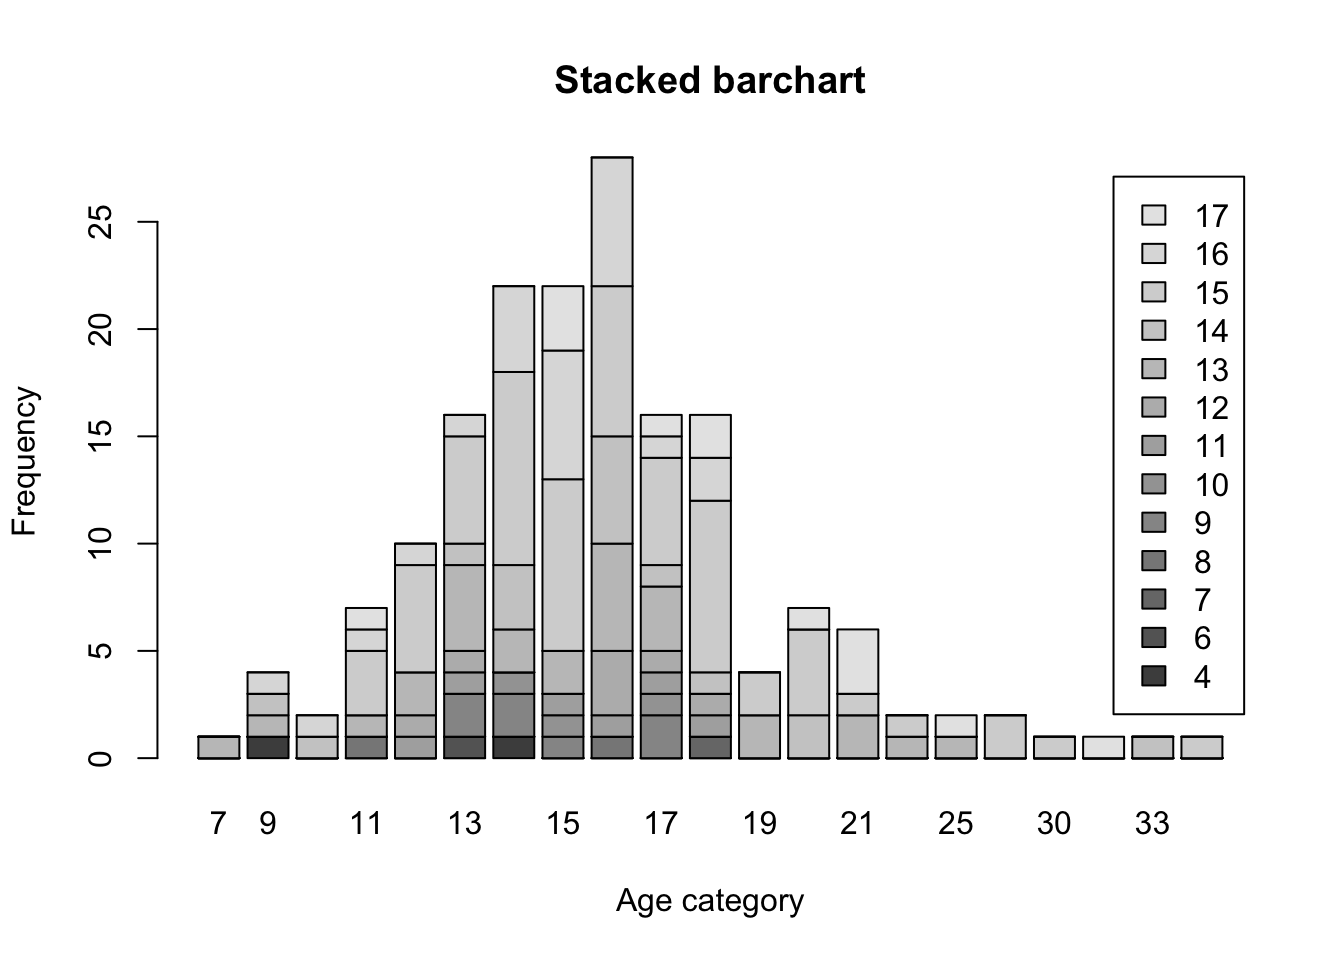
\includegraphics{Assignments_files/figure-latex/unnamed-chunk-22-1.pdf}

Earliest age range is 10.

\begin{Shaded}
\begin{Highlighting}[]
\FunctionTok{table}\NormalTok{(dat}\SpecialCharTok{$}\NormalTok{iralcage,dat}\SpecialCharTok{$}\NormalTok{age2)}
\end{Highlighting}
\end{Shaded}

\begin{verbatim}
##     
##       4  6  7  8  9 10 11 12 13 14 15 16 17
##   5   0  0  0  0  0  0  0  0  1  0  0  1  0
##   7   0  0  0  0  0  0  0  0  0  0  0  1  0
##   8   0  0  0  0  0  0  0  0  0  0  2  0  0
##   9   0  0  0  0  0  0  0  0  1  0  0  0  0
##   10  0  1  0  0  0  0  0  0  0  0  2  1  0
##   11  1  0  0  1  0  0  0  0  0  0  2  0  0
##   12  0  0  0  0  1  1  0  2  0  1 10  3  1
##   13  1  0  0  0  2  0  0  0  5  1  9  1  2
##   14  0  0  0  0  1  1  1  1  4  2  6  5  1
##   15  0  0  0  0  2  0  1  1  7  1  4  3  0
##   16  0  0  1  1  1  0  0  1  2  6  7  5  2
##   17  0  0  0  0  0  0  0  1  2  0  7  2  0
##   18  0  0  0  0  0  1  1  1  1  3 10  2  4
##   19  0  0  0  0  0  0  1  0  1  0  2  0  2
##   20  0  0  0  0  0  0  1  0  0  0  0  0  1
##   21  0  0  0  0  0  0  1  0  3  2  0  0  0
##   23  0  0  0  0  0  0  0  0  0  0  1  0  0
\end{verbatim}

\begin{Shaded}
\begin{Highlighting}[]
\FunctionTok{head}\NormalTok{(dat)}
\end{Highlighting}
\end{Shaded}

\begin{verbatim}
##   mjage cigage iralcage age2 sexatract speakengl irsex
## 1    14     50       14   16         1         1     1
## 2    11     14        5   13         2         1     2
## 3    12     35       12   15         2         1     2
## 4    16     18       18   14         1         1     1
## 5    14     16       14   16         4         1     1
## 6    12     16       18   15         4         1     2
\end{verbatim}

\begin{Shaded}
\begin{Highlighting}[]
\NormalTok{tab.ageiralcage }\OtherTok{\textless{}{-}} \FunctionTok{table}\NormalTok{(dat}\SpecialCharTok{$}\NormalTok{iralcage,dat}\SpecialCharTok{$}\NormalTok{age2)}
\FunctionTok{barplot}\NormalTok{(tab.ageiralcage,}
        \AttributeTok{main =} \StringTok{"Stacked barchart"}\NormalTok{,}
        \AttributeTok{xlab =} \StringTok{"Age category"}\NormalTok{, }\AttributeTok{ylab =} \StringTok{"Frequency"}\NormalTok{,}
        \AttributeTok{legend.text =} \FunctionTok{rownames}\NormalTok{(tab.ageiralcage),}
        \AttributeTok{beside =} \ConstantTok{FALSE}\NormalTok{) }\CommentTok{\# Stacked bars (default)}
\end{Highlighting}
\end{Shaded}

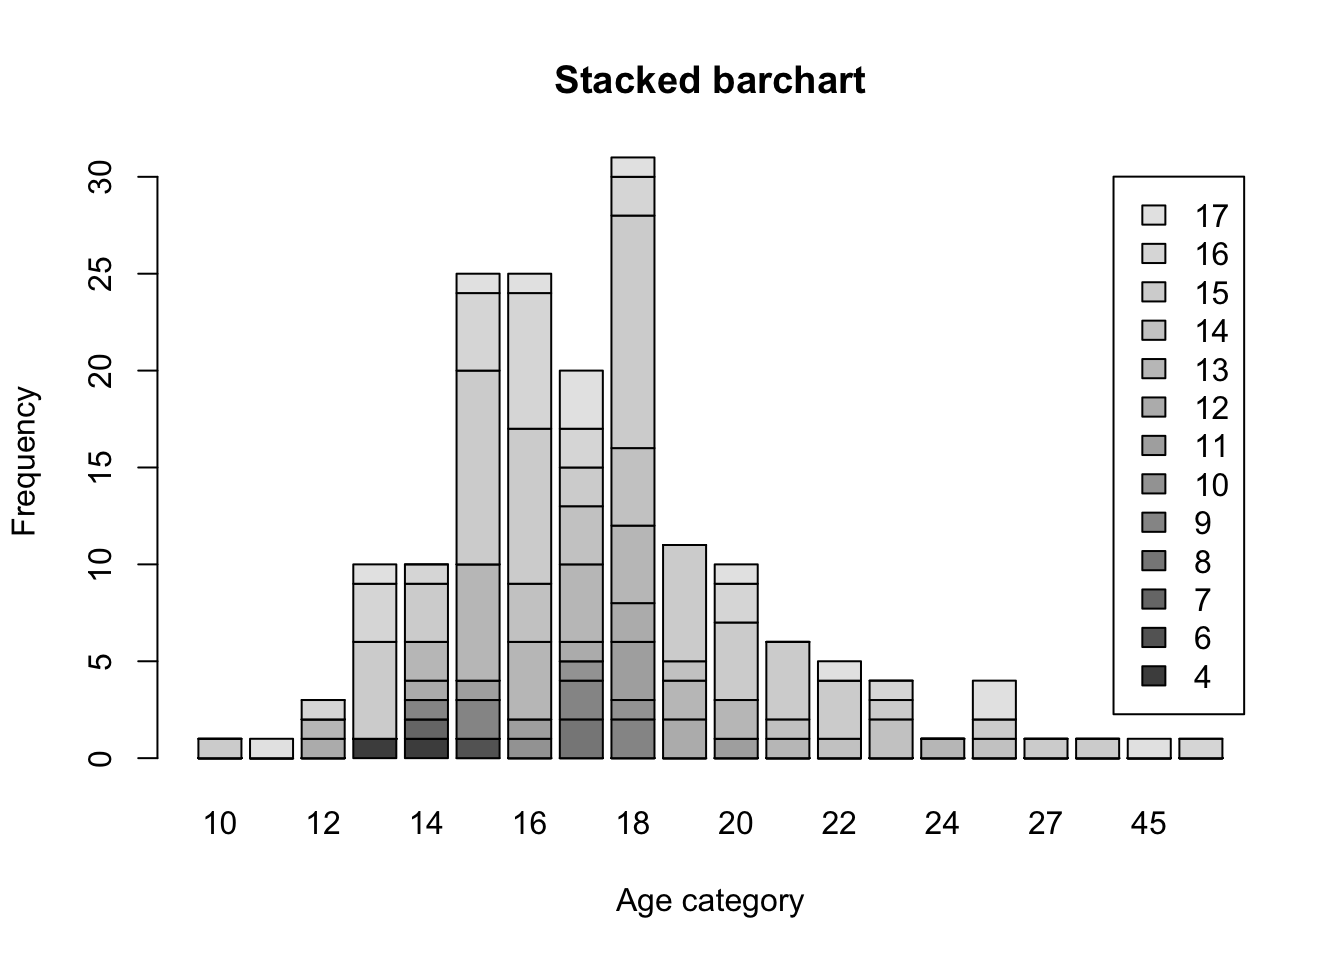
\includegraphics{Assignments_files/figure-latex/unnamed-chunk-23-1.pdf}

Earliest age range is 5.

\hypertarget{problem-5-sexual-attraction}{%
\subsection{Problem 5: Sexual
attraction}\label{problem-5-sexual-attraction}}

What does the distribution of sexual attraction look like? Is this what
you expected? What is the distribution of sexual attraction by gender?

\begin{Shaded}
\begin{Highlighting}[]
\FunctionTok{table}\NormalTok{(dat}\SpecialCharTok{$}\NormalTok{sexatract,dat}\SpecialCharTok{$}\NormalTok{irsex)}
\end{Highlighting}
\end{Shaded}

\begin{verbatim}
##     
##       1  2
##   1  82 54
##   2   3 13
##   3   0  9
##   4   1  2
##   5   2  1
##   6   1  0
##   99  2  1
\end{verbatim}

\begin{Shaded}
\begin{Highlighting}[]
\FunctionTok{head}\NormalTok{(dat)}
\end{Highlighting}
\end{Shaded}

\begin{verbatim}
##   mjage cigage iralcage age2 sexatract speakengl irsex
## 1    14     50       14   16         1         1     1
## 2    11     14        5   13         2         1     2
## 3    12     35       12   15         2         1     2
## 4    16     18       18   14         1         1     1
## 5    14     16       14   16         4         1     1
## 6    12     16       18   15         4         1     2
\end{verbatim}

\begin{Shaded}
\begin{Highlighting}[]
\NormalTok{tab.irsexatract }\OtherTok{\textless{}{-}} \FunctionTok{table}\NormalTok{(dat}\SpecialCharTok{$}\NormalTok{sexatract,dat}\SpecialCharTok{$}\NormalTok{irsex)}
\FunctionTok{barplot}\NormalTok{(tab.irsexatract,}
        \AttributeTok{main =} \StringTok{"Stacked barchart"}\NormalTok{,}
        \AttributeTok{xlab =} \StringTok{"Sexual Attraction"}\NormalTok{, }\AttributeTok{ylab =} \StringTok{"Frequency"}\NormalTok{,}
        \AttributeTok{legend.text =} \FunctionTok{rownames}\NormalTok{(tab.irsexatract),}
        \AttributeTok{beside =} \ConstantTok{FALSE}\NormalTok{) }\CommentTok{\# Stacked bars (default)}
\end{Highlighting}
\end{Shaded}

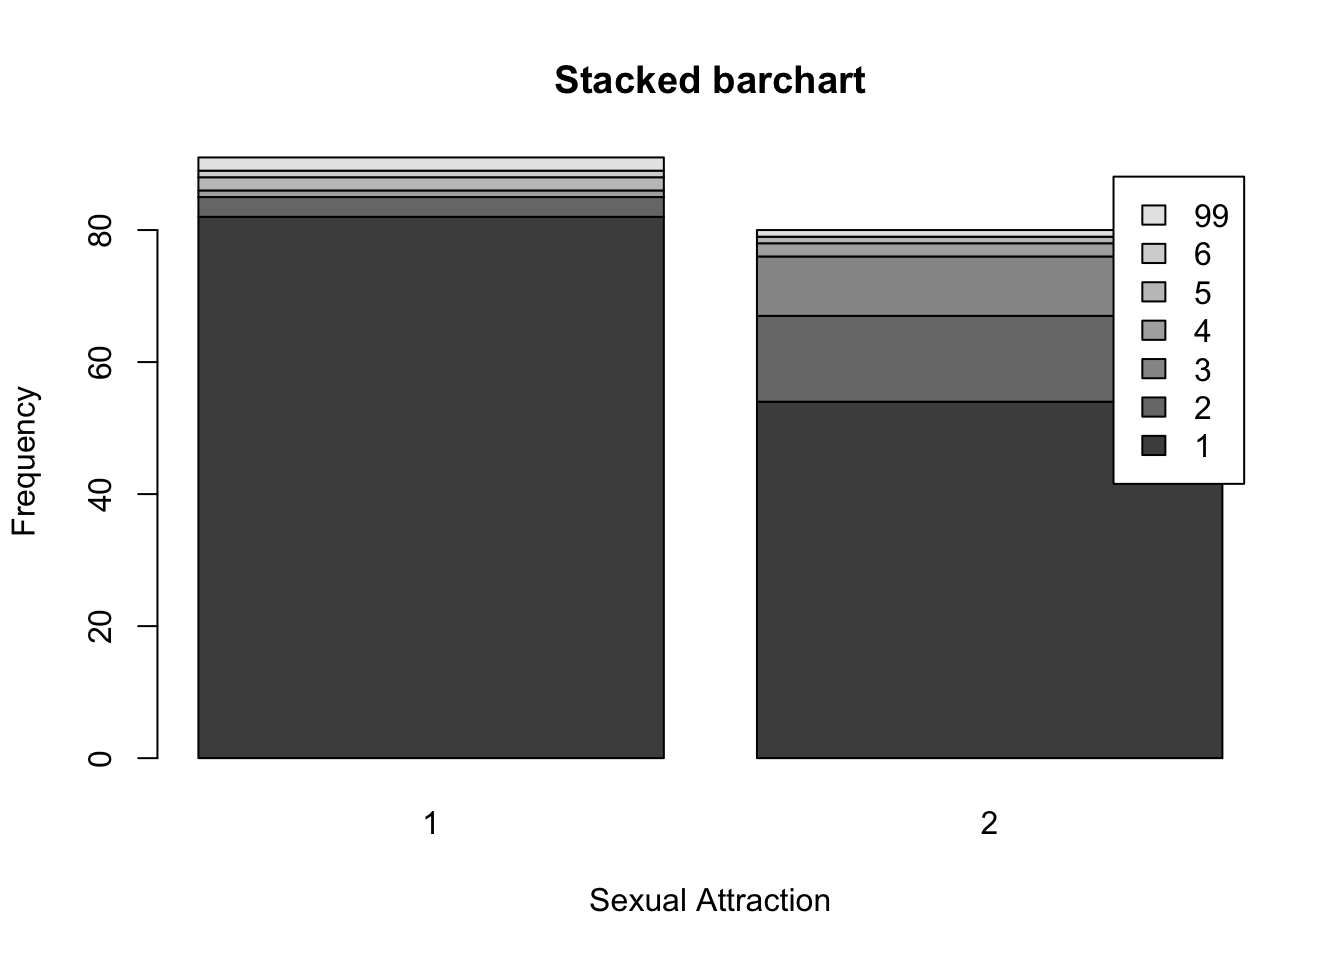
\includegraphics{Assignments_files/figure-latex/unnamed-chunk-24-1.pdf}

Answer: ``I am only attracted to the oppisote sex'' accounts for the
majority of both males and females, however it accounts for nearly all
men. From there, the numbers are very low. More women state they are as
equally attracted to men as they are to other women. The difference is
very minimal for those who selected ``I am mostly attracted to same
sex,'' ``I am only attracted to same sex,'' I am not sure," and those
who skipped the question. I am not surprised. There's a great deal of
non-binary, intersex, transgender, and other sexual identities outside
of male and female that aren't accounted for. Furthermore, these
individuals left out would most likely not be in the first category,
thus varying the data and evening out the distribution of the data.

\hypertarget{problem-6-english-speaking}{%
\subsection{Problem 6: English
speaking}\label{problem-6-english-speaking}}

What does the distribution of English speaking look like in the sample?
Is this what you might expect for a random sample of the US population?

\begin{Shaded}
\begin{Highlighting}[]
\FunctionTok{table}\NormalTok{(dat}\SpecialCharTok{$}\NormalTok{speakengl,dat}\SpecialCharTok{$}\NormalTok{irsex)}
\end{Highlighting}
\end{Shaded}

\begin{verbatim}
##    
##      1  2
##   1 84 77
##   2  7  1
##   3  0  2
\end{verbatim}

\begin{Shaded}
\begin{Highlighting}[]
\FunctionTok{head}\NormalTok{(dat)}
\end{Highlighting}
\end{Shaded}

\begin{verbatim}
##   mjage cigage iralcage age2 sexatract speakengl irsex
## 1    14     50       14   16         1         1     1
## 2    11     14        5   13         2         1     2
## 3    12     35       12   15         2         1     2
## 4    16     18       18   14         1         1     1
## 5    14     16       14   16         4         1     1
## 6    12     16       18   15         4         1     2
\end{verbatim}

\begin{Shaded}
\begin{Highlighting}[]
\NormalTok{tab.irsexspeakengl }\OtherTok{\textless{}{-}} \FunctionTok{table}\NormalTok{(dat}\SpecialCharTok{$}\NormalTok{speakengl,dat}\SpecialCharTok{$}\NormalTok{irsex)}
\FunctionTok{barplot}\NormalTok{(tab.irsexspeakengl,}
        \AttributeTok{main =} \StringTok{"Stacked barchart"}\NormalTok{,}
        \AttributeTok{xlab =} \StringTok{"Speak English"}\NormalTok{, }\AttributeTok{ylab =} \StringTok{"Frequency"}\NormalTok{,}
        \AttributeTok{legend.text =} \FunctionTok{rownames}\NormalTok{(tab.irsexspeakengl),}
        \AttributeTok{beside =} \ConstantTok{FALSE}\NormalTok{) }\CommentTok{\# Stacked bars (default)}
\end{Highlighting}
\end{Shaded}

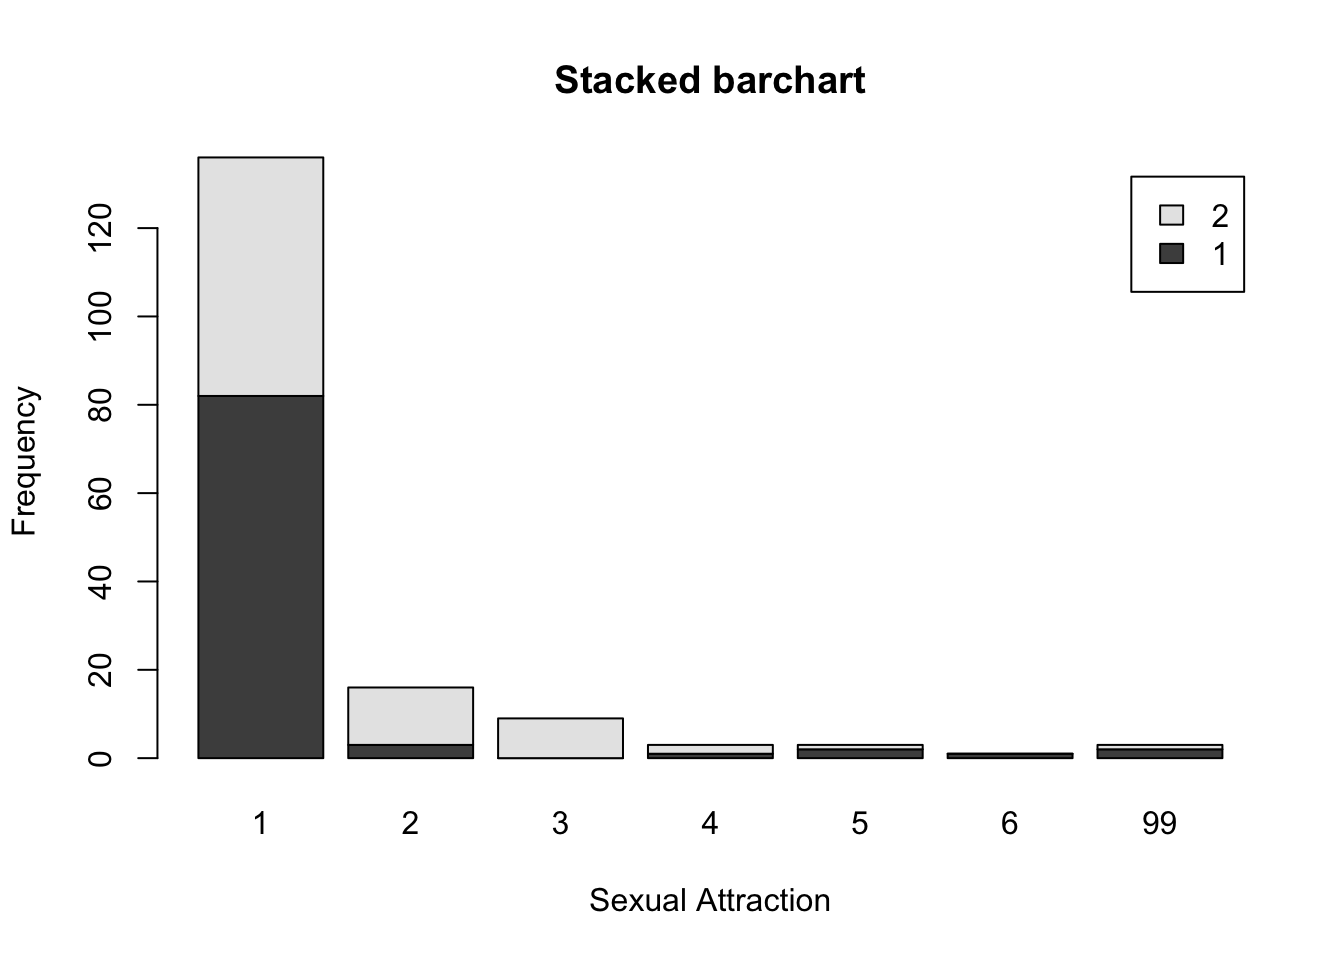
\includegraphics{Assignments_files/figure-latex/unnamed-chunk-25-1.pdf}

Answer: There is an extremely high frequency of individuals that can
speak english very well. It accounts for nearly all men and women
respectively. A small group of individuals stated they spoke english
well (7 men and 1 woman) and 2 women stated they spoke english not well.

Are there more English speaker females or males?

Answer: There are more male English speakers.

\#Assignment 3

Load the data.

\begin{Shaded}
\begin{Highlighting}[]
\FunctionTok{library}\NormalTok{(readr)}
\FunctionTok{library}\NormalTok{(knitr)}
\NormalTok{dat.crime }\OtherTok{\textless{}{-}} \FunctionTok{read\_delim}\NormalTok{(}\StringTok{"crime\_simple.txt"}\NormalTok{, }\AttributeTok{delim =} \StringTok{"}\SpecialCharTok{\textbackslash{}t}\StringTok{"}\NormalTok{)}
\end{Highlighting}
\end{Shaded}

\begin{verbatim}
## Rows: 47 Columns: 14
\end{verbatim}

\begin{verbatim}
## -- Column specification --------------------------------------------------------
## Delimiter: "\t"
## dbl (14): R, Age, S, Ed, Ex0, Ex1, LF, M, N, NW, U1, U2, W, X
\end{verbatim}

\begin{verbatim}
## 
## i Use `spec()` to retrieve the full column specification for this data.
## i Specify the column types or set `show_col_types = FALSE` to quiet this message.
\end{verbatim}

This is a dataset from a textbook by Brian S. Everitt about crime in the
US in 1960. The data originate from the Uniform Crime Report of the FBI
and other government sources. The data for 47 states of the USA are
given.

Here is the codebook:

R: Crime rate: \# of offenses reported to police per million population

Age: The number of males of age 14-24 per 1000 population

S: Indicator variable for Southern states (0 = No, 1 = Yes)

Ed: Mean of years of schooling x 10 for persons of age 25 or older

Ex0: 1960 per capita expenditure on police by state and local government

Ex1: 1959 per capita expenditure on police by state and local government

LF: Labor force participation rate per 1000 civilian urban males age
14-24

M: The number of males per 1000 females

N: State population size in hundred thousands

NW: The number of non-whites per 1000 population

U1: Unemployment rate of urban males per 1000 of age 14-24

U2: Unemployment rate of urban males per 1000 of age 35-39

W: Median value of transferable goods and assets or family income in
tens of \$

X: The number of families per 1000 earning below 1/2 the median income

We are interested in checking whether the reported crime rate (\# of
offenses reported to police per million population) and the average
education (mean number of years of schooling for persons of age 25 or
older) are related.

\begin{enumerate}
\def\labelenumi{\arabic{enumi}.}
\tightlist
\item
  How many observations are there in the dataset? To what does each
  observation correspond?
\end{enumerate}

\textbf{There are 47 observations in this dataset. The observations
correspond to 47 U.S. states. This information is given in the
introduction of the codebook. }

\begin{enumerate}
\def\labelenumi{\arabic{enumi}.}
\setcounter{enumi}{1}
\tightlist
\item
  Draw a scatterplot of the two variables. Calculate the correlation
  between the two variables. Can you come up with an explanation for
  this relationship?
\end{enumerate}

\begin{Shaded}
\begin{Highlighting}[]
\NormalTok{x }\OtherTok{\textless{}{-}}\NormalTok{ dat.crime}\SpecialCharTok{$}\NormalTok{R}
\NormalTok{y }\OtherTok{\textless{}{-}}\NormalTok{ dat.crime}\SpecialCharTok{$}\NormalTok{Ed}
\FunctionTok{plot}\NormalTok{(x, y, }\AttributeTok{main =} \StringTok{"Scatterplot  of Crime Rate vs. Average Education"}\NormalTok{,}
     \AttributeTok{xlab =} \StringTok{"Reported Crime Rate"}\NormalTok{, }\AttributeTok{ylab =} \StringTok{"Average Education"}\NormalTok{,}
     \AttributeTok{pch =} \DecValTok{19}\NormalTok{, }\AttributeTok{frame =} \ConstantTok{FALSE}\NormalTok{)}
\end{Highlighting}
\end{Shaded}

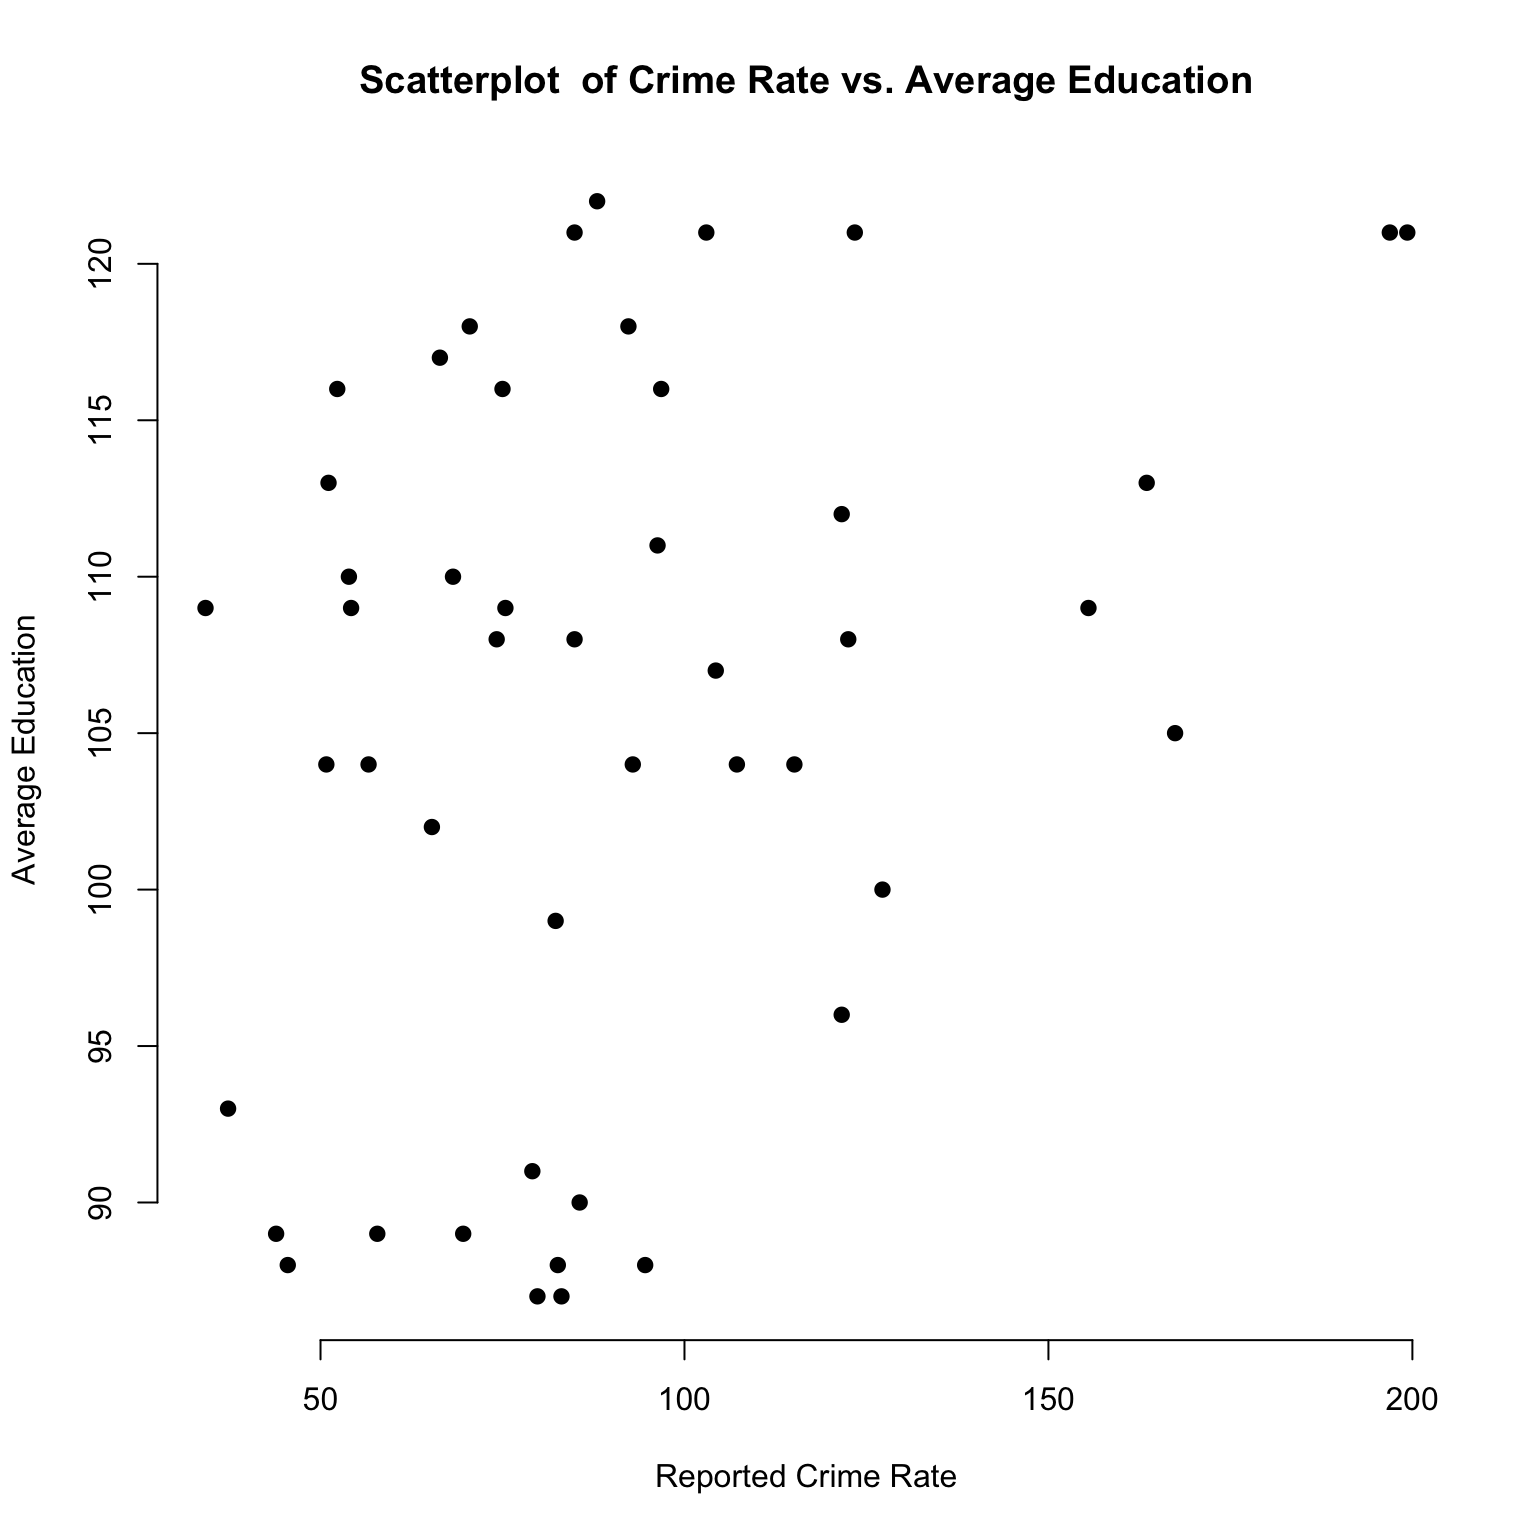
\includegraphics{Assignments_files/figure-latex/unnamed-chunk-28-1.pdf}

\textbf{It appears that my initial scatterplot organizes the data in a
way that is hard to read so I inverted the variables.}

\begin{Shaded}
\begin{Highlighting}[]
\NormalTok{x }\OtherTok{\textless{}{-}}\NormalTok{ dat.crime}\SpecialCharTok{$}\NormalTok{Ed}
\NormalTok{y }\OtherTok{\textless{}{-}}\NormalTok{ dat.crime}\SpecialCharTok{$}\NormalTok{R}
\FunctionTok{plot}\NormalTok{(x, y, }\AttributeTok{main =} \StringTok{"Scatterplot of Average Education vs. Reported Crime Rate"}\NormalTok{,}
     \AttributeTok{xlab =} \StringTok{"Average Education (mean number of years of schooling for persons of age 25 or older)"}\NormalTok{, }\AttributeTok{ylab =} \StringTok{"Reported Crime Rate (\# of offenses reported to police per million population)"}\NormalTok{,}
     \AttributeTok{pch =} \DecValTok{19}\NormalTok{, }\AttributeTok{frame =} \ConstantTok{FALSE}\NormalTok{)}
\end{Highlighting}
\end{Shaded}

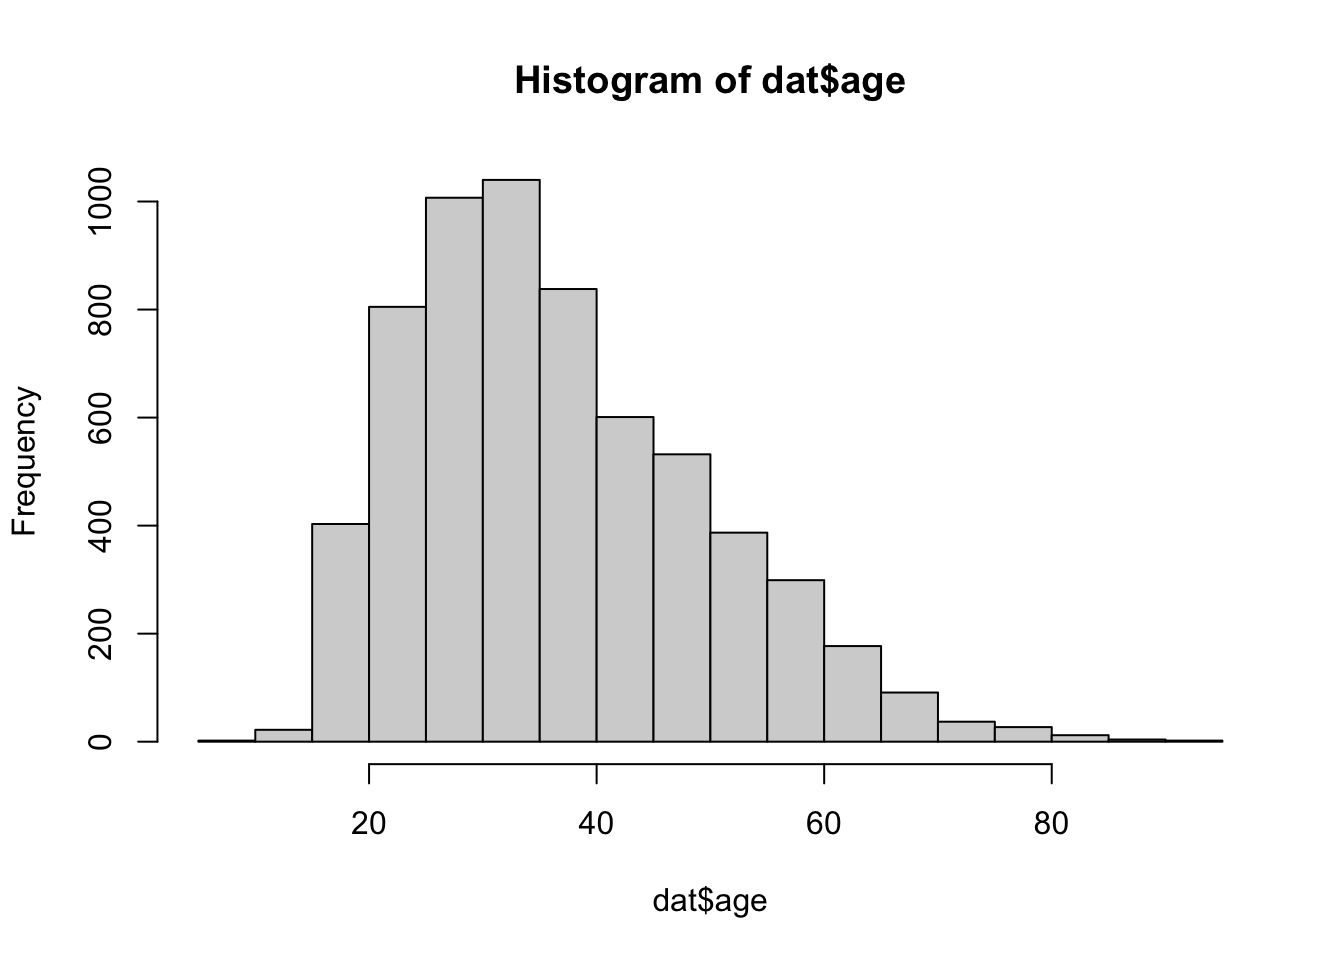
\includegraphics{Assignments_files/figure-latex/unnamed-chunk-29-1.pdf}

\begin{Shaded}
\begin{Highlighting}[]
\FunctionTok{cor}\NormalTok{(x, y, }\AttributeTok{method =} \FunctionTok{c}\NormalTok{(}\StringTok{"pearson"}\NormalTok{, }\StringTok{"kendall"}\NormalTok{, }\StringTok{"spearman"}\NormalTok{))}
\end{Highlighting}
\end{Shaded}

\begin{verbatim}
## [1] 0.3228349
\end{verbatim}

\textbf{The correlation coeeficient = 0.3228349. This is reflected in
the scatter plot because the data certainly does not follow the line of
best fit and there is a very weak correlation between the two variables.
The only basis someone would have to have to assume there'd be a
correlation is that those who are more educated are smart enough to not
commit crimes. In this case, they are assuming intellect also signifies
morality, which is not always the case. Also, there's no accounting of
potentially unreported cases that would be committed by highly
intellectual criminals. I think there are too many factors in play, such
as access to schooling, racial bias, unreported cases, etc for their to
be a strong correlation between the two variables. }

\begin{enumerate}
\def\labelenumi{\arabic{enumi}.}
\setcounter{enumi}{2}
\tightlist
\item
  Regress reported crime rate (y) on average education (x) and call this
  linear model \texttt{crime.lm} and write the summary of the regression
  by using this code, which makes it look a little nicer
  \texttt{\{r,\ eval=FALSE\}\ kable(summary(crime.lm)\$coef,\ digits\ =\ 2)}.
\end{enumerate}

\begin{Shaded}
\begin{Highlighting}[]
\NormalTok{crime.lm}\OtherTok{\textless{}{-}} \FunctionTok{lm}\NormalTok{(R }\SpecialCharTok{\textasciitilde{}}\NormalTok{ Ed, }\AttributeTok{data =}\NormalTok{ dat.crime)}
\FunctionTok{summary}\NormalTok{(crime.lm)}
\end{Highlighting}
\end{Shaded}

\begin{verbatim}
## 
## Call:
## lm(formula = R ~ Ed, data = dat.crime)
## 
## Residuals:
##     Min      1Q  Median      3Q     Max 
## -60.061 -27.125  -4.654  17.133  91.646 
## 
## Coefficients:
##             Estimate Std. Error t value Pr(>|t|)  
## (Intercept) -27.3967    51.8104  -0.529   0.5996  
## Ed            1.1161     0.4878   2.288   0.0269 *
## ---
## Signif. codes:  0 '***' 0.001 '**' 0.01 '*' 0.05 '.' 0.1 ' ' 1
## 
## Residual standard error: 37.01 on 45 degrees of freedom
## Multiple R-squared:  0.1042, Adjusted R-squared:  0.08432 
## F-statistic: 5.236 on 1 and 45 DF,  p-value: 0.02688
\end{verbatim}

\begin{enumerate}
\def\labelenumi{\arabic{enumi}.}
\setcounter{enumi}{3}
\tightlist
\item
  Are the four assumptions of linear regression satisfied? To answer
  this, draw the relevant plots. (Write a maximum of one sentence per
  assumption.)
\end{enumerate}

\begin{Shaded}
\begin{Highlighting}[]
\FunctionTok{install.packages}\NormalTok{(}\StringTok{"ggplot2"}\NormalTok{,}\AttributeTok{repos =} \StringTok{"http://cran.us.r{-}project.org"}\NormalTok{)}
\end{Highlighting}
\end{Shaded}

\begin{verbatim}
## 
## The downloaded binary packages are in
##  /var/folders/nh/m2s_dxnj099clcww6tpc2vy00000gn/T//Rtmpa8F00e/downloaded_packages
\end{verbatim}

\begin{Shaded}
\begin{Highlighting}[]
\FunctionTok{install.packages}\NormalTok{(}\StringTok{"ggfortify"}\NormalTok{,}\AttributeTok{repos =} \StringTok{"http://cran.us.r{-}project.org"}\NormalTok{)}
\end{Highlighting}
\end{Shaded}

\begin{verbatim}
## 
## The downloaded binary packages are in
##  /var/folders/nh/m2s_dxnj099clcww6tpc2vy00000gn/T//Rtmpa8F00e/downloaded_packages
\end{verbatim}

\begin{Shaded}
\begin{Highlighting}[]
\FunctionTok{library}\NormalTok{ (ggplot2)}
\FunctionTok{library}\NormalTok{(ggfortify)}
\FunctionTok{autoplot}\NormalTok{(crime.lm)}
\end{Highlighting}
\end{Shaded}

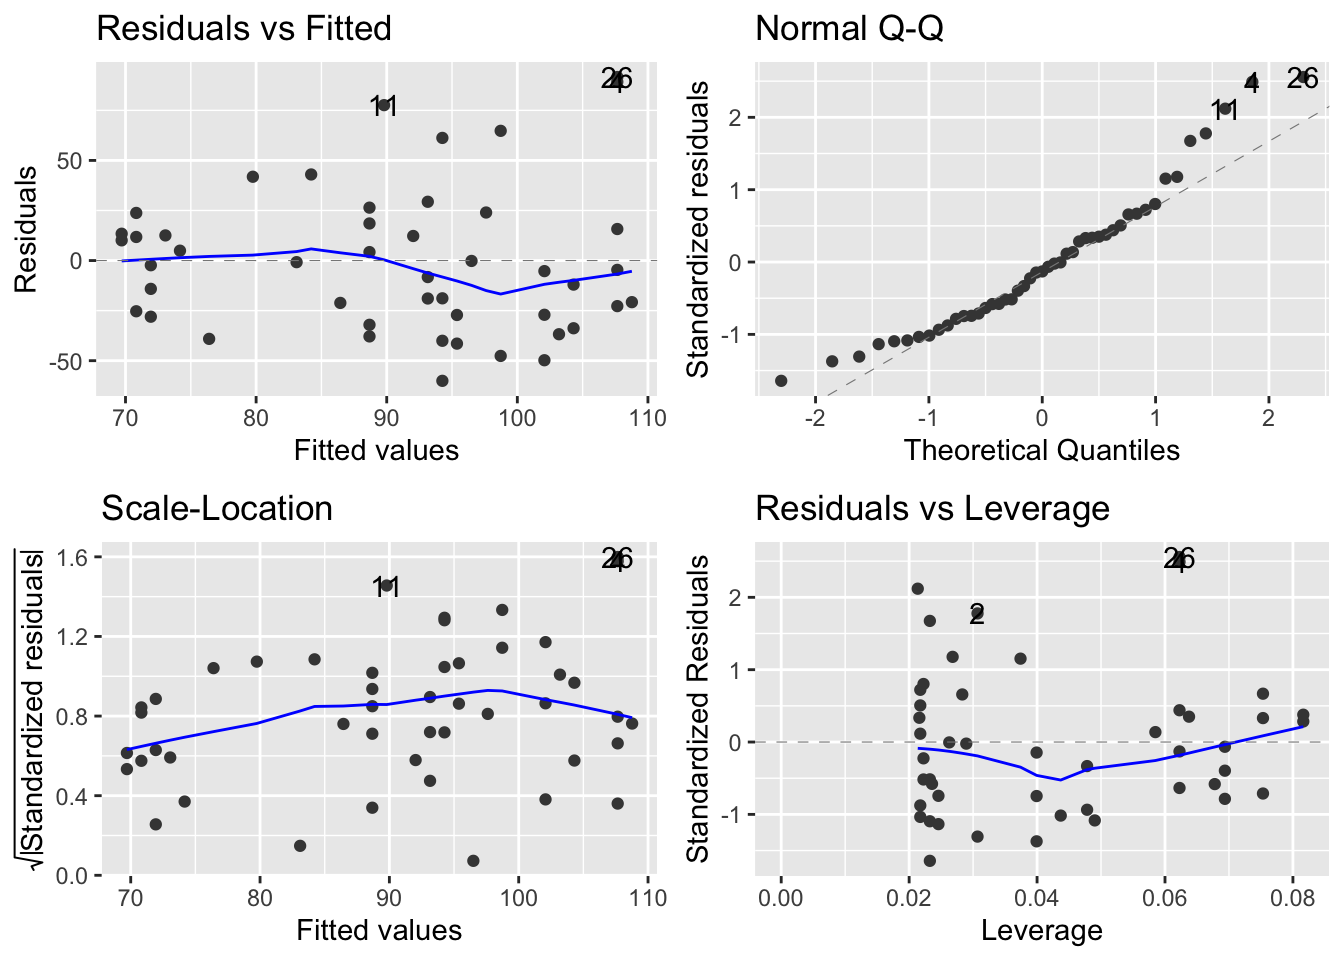
\includegraphics{Assignments_files/figure-latex/unnamed-chunk-31-1.pdf}

\begin{Shaded}
\begin{Highlighting}[]
\FunctionTok{plot}\NormalTok{(crime.lm, }\DecValTok{1}\NormalTok{)}
\end{Highlighting}
\end{Shaded}

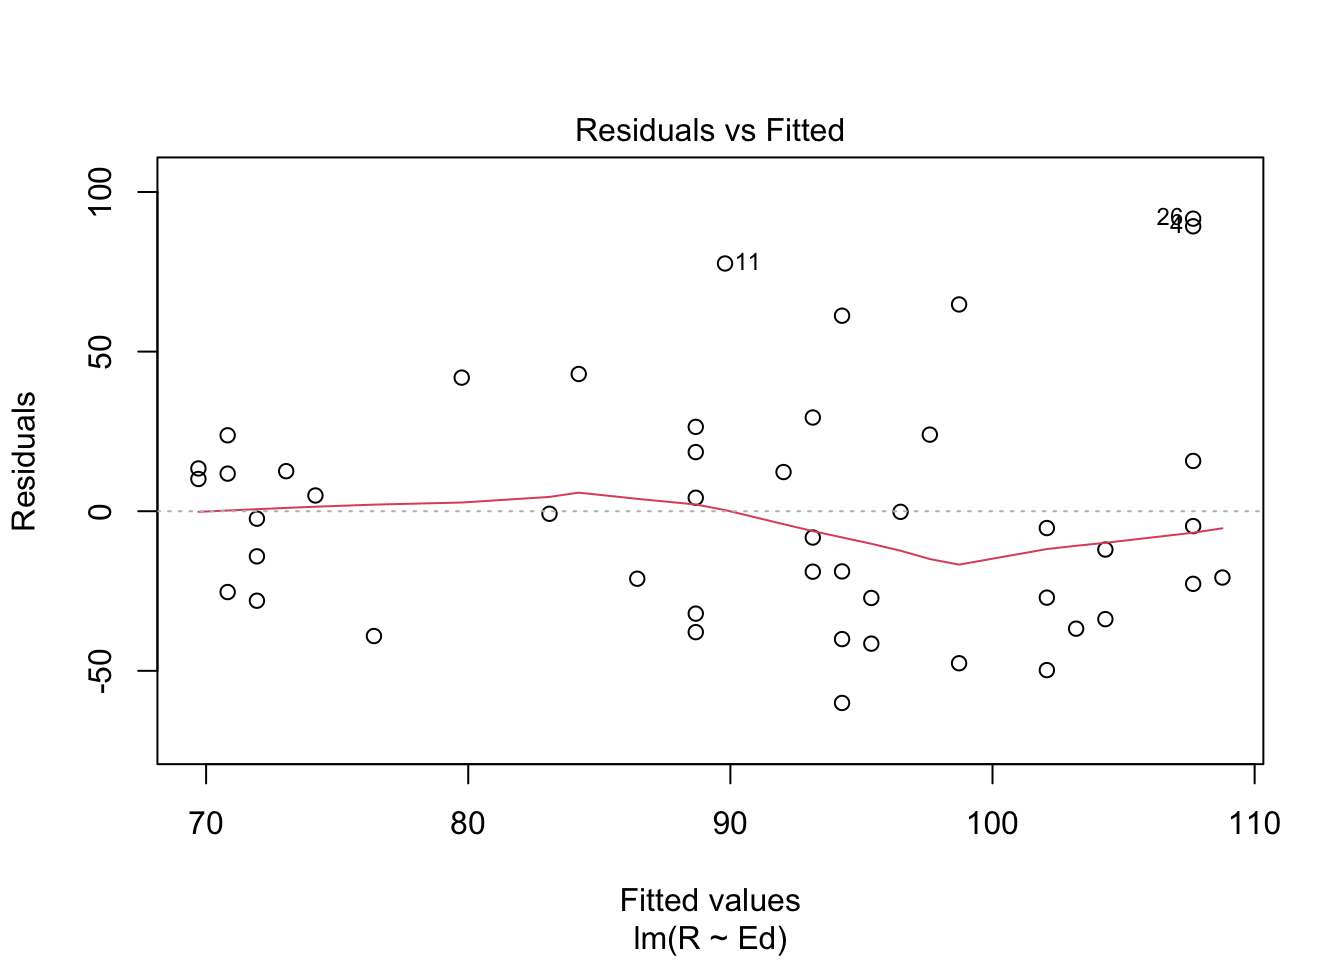
\includegraphics{Assignments_files/figure-latex/unnamed-chunk-31-2.pdf}

\begin{Shaded}
\begin{Highlighting}[]
\FunctionTok{plot}\NormalTok{(crime.lm, }\DecValTok{3}\NormalTok{)}
\end{Highlighting}
\end{Shaded}

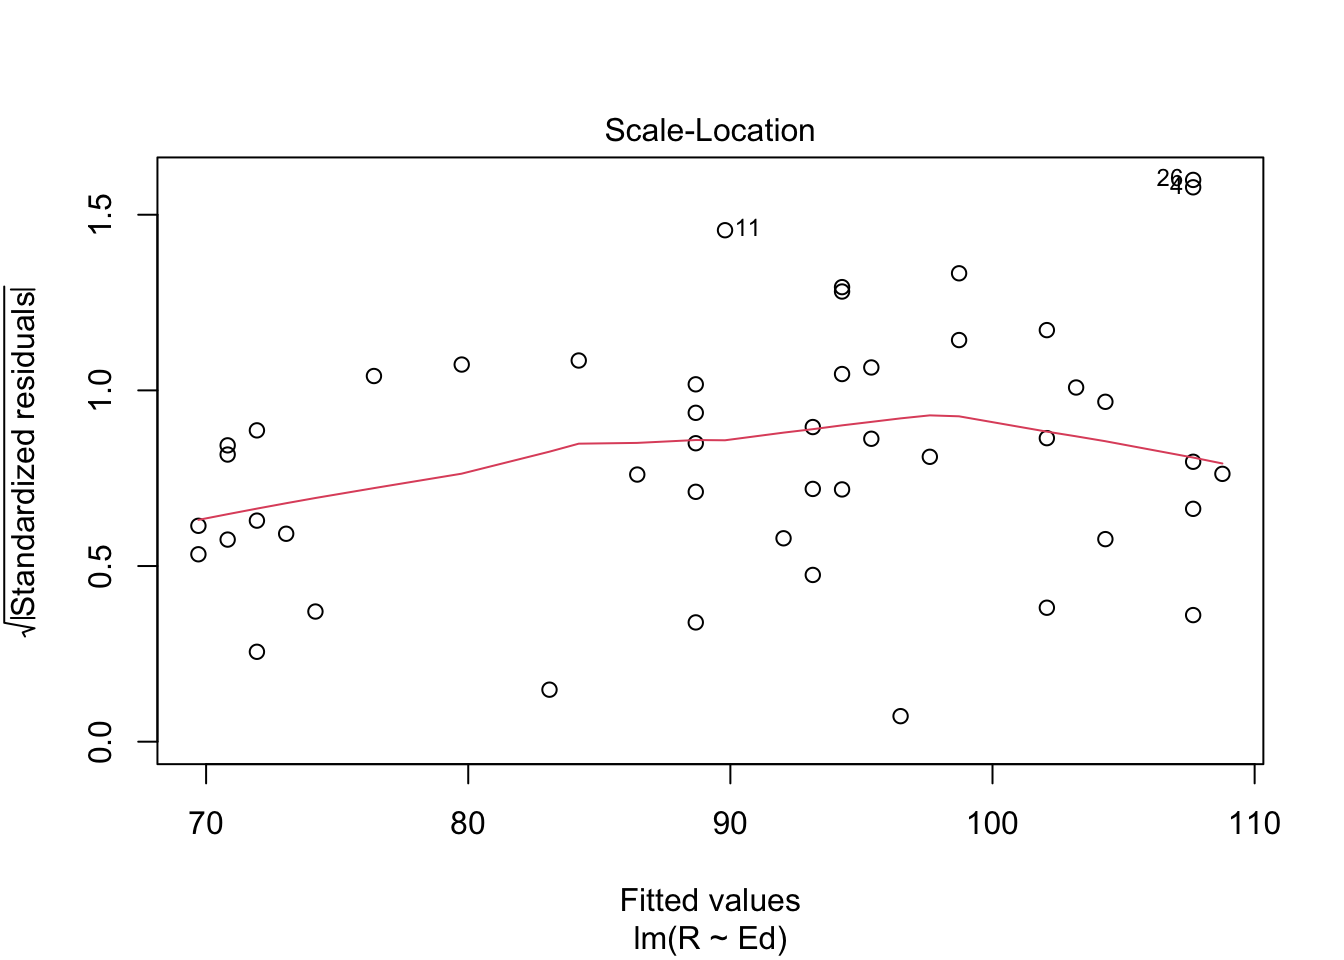
\includegraphics{Assignments_files/figure-latex/unnamed-chunk-31-3.pdf}

\begin{Shaded}
\begin{Highlighting}[]
\FunctionTok{plot}\NormalTok{(crime.lm, }\DecValTok{2}\NormalTok{)}
\end{Highlighting}
\end{Shaded}

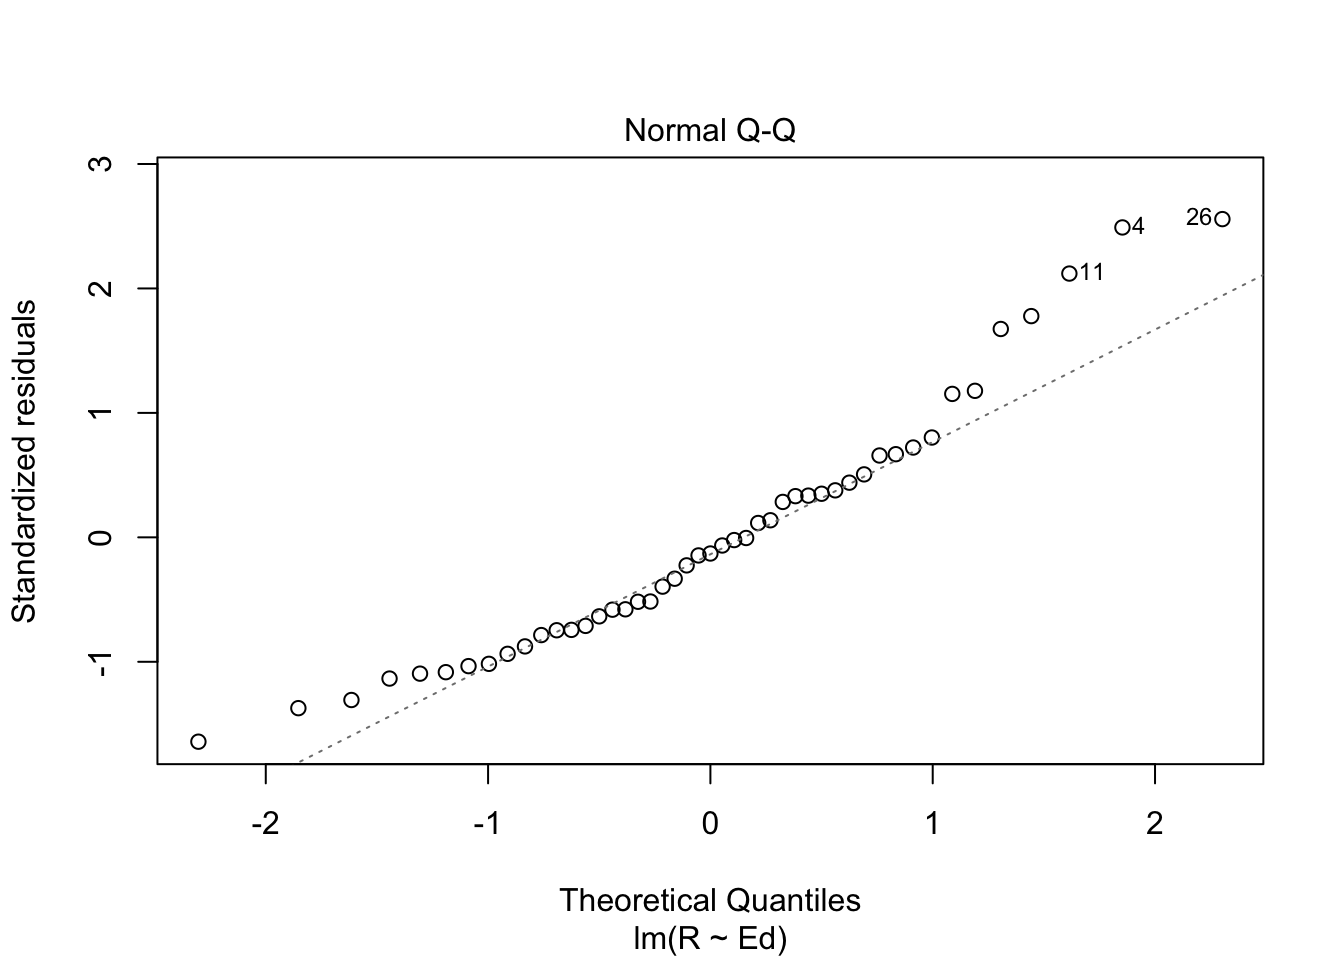
\includegraphics{Assignments_files/figure-latex/unnamed-chunk-31-4.pdf}

\begin{Shaded}
\begin{Highlighting}[]
\FunctionTok{plot}\NormalTok{(crime.lm, }\DecValTok{5}\NormalTok{)}
\end{Highlighting}
\end{Shaded}

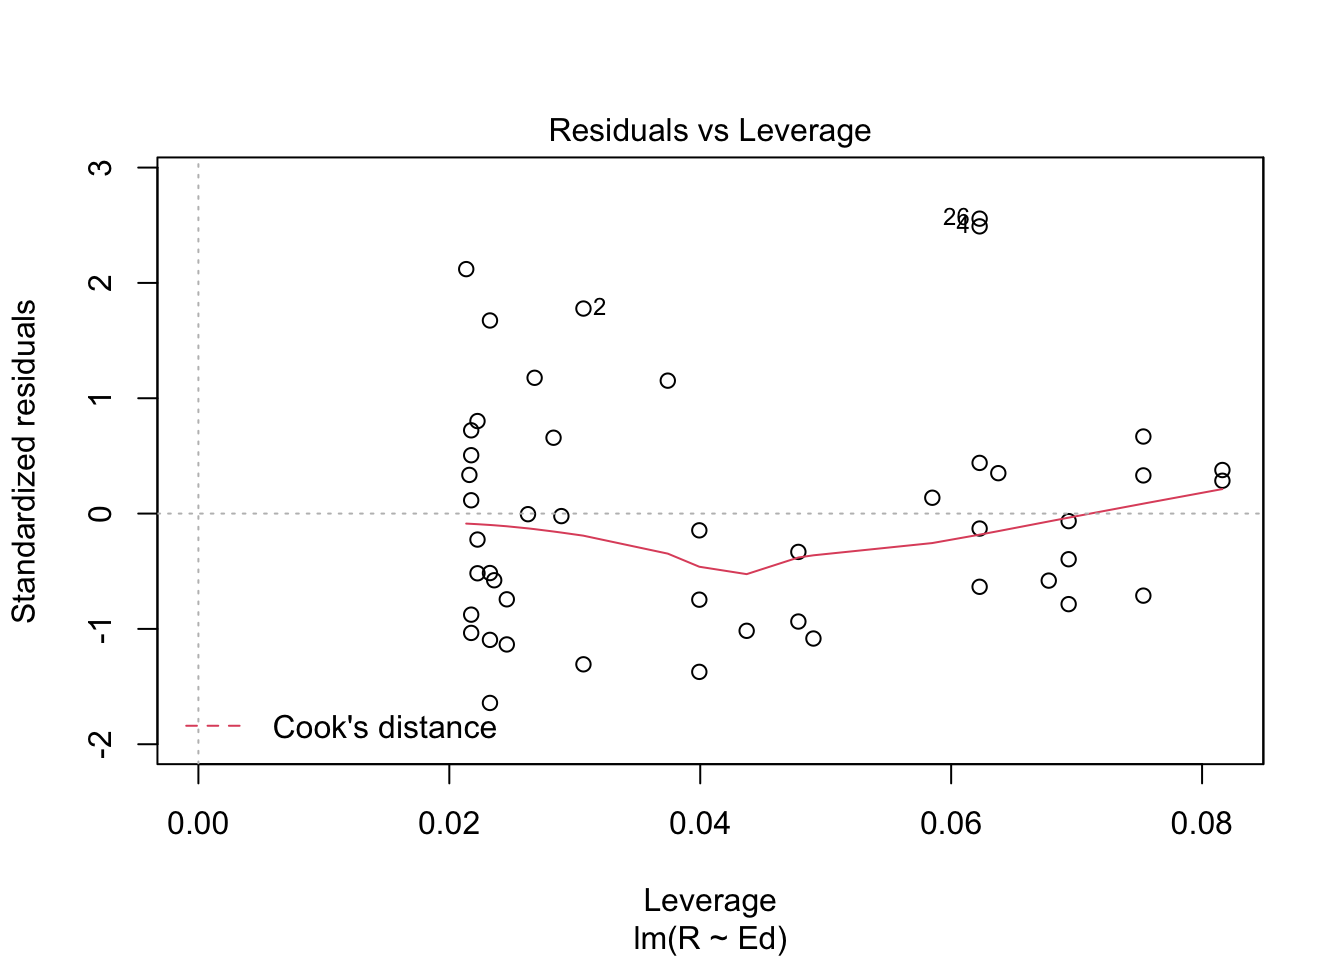
\includegraphics{Assignments_files/figure-latex/unnamed-chunk-31-5.pdf}

\textbf{The assumption of linearity is satisfied because the residual
plot shows no fitted pattern, as in the red line is approximately
horizontal at zero. The assumption of homoscedasticity is not satisfied
because there isn't a horizontal line with equally spread points since
the variability of the residual points increases for a bit of time then
decreases with the value of the fitted outcome variable, suggesting
non-constant variances in the residuals errors (or
heteroscedasticity).The assumption of normality is not satisfied because
all the data points do not fall on the reference line. The assumption of
independence is not satisfied because the slight patterns shown
indicates a linear relationship between the predictors and the outcome
variable\ldots{}}

\begin{enumerate}
\def\labelenumi{\arabic{enumi}.}
\setcounter{enumi}{4}
\tightlist
\item
  Is the relationship between reported crime and average education
  statistically significant? Report the estimated coefficient of the
  slope, the standard error, and the p-value. What does it mean for the
  relationship to be statistically significant?
\end{enumerate}

\textbf{The relationship between reported crime and average education is
not statistically significant. In fact, neither the assumption of
homoscedasticity, normality, nor independence is satisfied, and so we
cannot rely on the linear model to make conclusions about the data. The
estimated coefficient of the slope = 1.1161, the standard error=0.4878
(residual standard error =37.01 on 45 degrees of freedom) and the p
value =0.02688. For the relationship to be statistically significant, we
would have a better chance of being right in finding that a relationship
exists between two variables. In other words, the probability of being
wrong is small.}

\begin{enumerate}
\def\labelenumi{\arabic{enumi}.}
\setcounter{enumi}{5}
\tightlist
\item
  How are reported crime and average education related? In other words,
  for every unit increase in average education, how does reported crime
  rate change (per million) per state?
\end{enumerate}

\textbf{for every unit increase in average education, reported crime
rate increases 1.1161 (per million) per state. The slope which
determines this answer was calculated in the problem above.}

\begin{enumerate}
\def\labelenumi{\arabic{enumi}.}
\setcounter{enumi}{6}
\tightlist
\item
  Can you conclude that if individuals were to receive more education,
  then crime will be reported more often? Why or why not?
\end{enumerate}

\textbf{The data does not give us any information to answer this
question, especially because of the lack of correlation between the
variables. However, based on other studies and their statistical
findings, I would say for individuals who received more education, their
crimes would be reported less. They are also not likely to be committing
crimes that would be detected by the everyday, typical officer. They'd
also be more likely to commit the crime in a more methodical and
rational way so as not to get caught..}

\#Assignment 4

\#Data Visualization 3:
\url{https://r4ds.had.co.nz/data-visualisation.html\#first-steps}

This code loads the tidyverse, an opinionated collection of R packages.

library(tidyverse) \#\textgreater{} ── Attaching packages
─────────────────────────────────────── tidyverse 1.3.0 ──
\#\textgreater{} ✔ ggplot2 3.3.2 ✔ purrr 0.3.4 \#\textgreater{} ✔ tibble
3.0.3 ✔ dplyr 1.0.2 \#\textgreater{} ✔ tidyr 1.1.2 ✔ stringr 1.4.0
\#\textgreater{} ✔ readr 1.4.0 ✔ forcats 0.5.0 \#\textgreater{} ──
Conflicts ──────────────────────────────────────────
tidyverse\_conflicts() ── \#\textgreater{} ✖ dplyr::filter() masks
stats::filter() \#\textgreater{} ✖ dplyr::lag() masks stats::lag()

This code installs the package ``tidyverse'' then loads the library.

install.packages(``tidyverse'') library(tidyverse)

This code tests your answer with the mpg data frame (a rectuangular
collection of variables and observations) found in ggplot2 (aka
ggplot2::mpg).

mpg \#\textgreater{} \# A tibble: 234 x 11 \#\textgreater{} manufacturer
model displ year cyl trans drv cty hwy fl class \#\textgreater{}
\#\textgreater{} 1 audi a4 1.8 1999 4 auto(l5) f 18 29 p compa\ldots{}
\#\textgreater{} 2 audi a4 1.8 1999 4 manual(m5) f 21 29 p compa\ldots{}
\#\textgreater{} 3 audi a4 2 2008 4 manual(m6) f 20 31 p compa\ldots{}
\#\textgreater{} 4 audi a4 2 2008 4 auto(av) f 21 30 p compa\ldots{}
\#\textgreater{} 5 audi a4 2.8 1999 6 auto(l5) f 16 26 p compa\ldots{}
\#\textgreater{} 6 audi a4 2.8 1999 6 manual(m5) f 18 26 p compa\ldots{}
\#\textgreater{} \# \ldots{} with 228 more rows

This code plots the graph. ggplot() creates a coordinate system that you
can add layers to. The first argument of ggplot() is the dataset to use
in the graph. The function geom\_point() adds a layer of points to your
plot, which creates a scatterplot.

ggplot(data = mpg) + geom\_point(mapping = aes(x = displ, y = hwy))

This code makes a graph because it replaces the bracketed sections in
the code below with a dataset, a geom function, or a collection of
mappings.

ggplot(data = ) + (mapping = aes())

You can add a third variable, like class, to a two dimensional
scatterplot by mapping it to an aesthetic. An aesthetic is a visual
property of the objects in your plot. Aesthetics include things like the
size, the shape, or the color of your points.

ggplot(data = mpg) + geom\_point(mapping = aes(x = displ, y = hwy, color
= class))

ggplot(data = mpg) + geom\_point(mapping = aes(x = displ, y = hwy, size
= class)) \#\textgreater{} Warning: Using size for a discrete variable
is not advised.

This code conveys information about your data by mapping the aesthetics
in your plot to the variables in your dataset.To map an aesthetic to a
variable, associate the name of the aesthetic to the name of the
variable inside aes(). ggplot2 will automatically assign a unique level
of the aesthetic (here a unique color) to each unique value of the
variable, a process known as scaling. ggplot2 will also add a legend
that explains which levels correspond to which values. In the above
example, we mapped class to the color aesthetic, but we could have
mapped class to the size aesthetic in the same way. In this case, the
exact size of each point would reveal its class affiliation. We get a
warning here, because mapping an unordered variable (class) to an
ordered aesthetic (size) is not a good idea.

This code controls the transparency of the points and the shape
aesthetic, which controls the shape of the points.

\# Left ggplot(data = mpg) + geom\_point(mapping = aes(x = displ, y =
hwy, alpha = class))

\# Right ggplot(data = mpg) + geom\_point(mapping = aes(x = displ, y =
hwy, shape = class))

This code sets the aesthetic properties manually (i.e.~color size,
shape, etc.) ggplot(data = mpg) + geom\_point(mapping = aes(x = displ, y
= hwy), color = ``blue'')

This code facets your plot by a single variable. Facets are subplots
that display individual subsets of the data. The first argument of
facet\_wrap() should be a formula, which you create with
\textasciitilde{} followed by a variable name (here ``formula'' is the
name of a data structure in R, not a synonym for ``equation''). The
variable that you pass to facet\_wrap() should be discrete.

ggplot(data = mpg) + geom\_point(mapping = aes(x = displ, y = hwy)) +
facet\_wrap(\textasciitilde{} class, nrow = 2)

This code facets your plot on the combination of two variables. The
first argument of facet\_grid() is also a formula. This time the formula
should contain two variable names separated by a \textasciitilde. If you
prefer to not facet in the rows or columns dimension, use a . instead of
a variable name, e.g.~+ facet\_grid(. \textasciitilde{} cyl).

ggplot(data = mpg) + geom\_point(mapping = aes(x = displ, y = hwy)) +
facet\_grid(drv \textasciitilde{} cyl)

ggplot(data = mpg) + geom\_point(mapping = aes(x = drv, y = cyl))

ggplot(data = mpg) + geom\_point(mapping = aes(x = displ, y = hwy)) +
facet\_grid(drv \textasciitilde{} .)

ggplot(data = mpg) + geom\_point(mapping = aes(x = displ, y = hwy)) +
facet\_grid(. \textasciitilde{} cyl)

This code changes the geom in your plot. \# left ggplot(data = mpg) +
geom\_point(mapping = aes(x = displ, y = hwy))

\# right ggplot(data = mpg) + geom\_smooth(mapping = aes(x = displ, y =
hwy))

This code sets the linetype of a line for each unique value of the
variable that you map to linetype. ggplot(data = mpg) +
geom\_smooth(mapping = aes(x = displ, y = hwy, linetype = drv))

This code sets the group aesthetic to a categorical variable to draw
multiple objects. ggplot2 will draw a separate object for each unique
value of the grouping variable. ggplot(data = mpg) +
geom\_smooth(mapping = aes(x = displ, y = hwy))

This code displays multiple geoms in the same plot. ggplot(data = mpg) +
geom\_point(mapping = aes(x = displ, y = hwy)) + geom\_smooth(mapping =
aes(x = displ, y = hwy))

This code produces the same plot as the previous code. ggplot(data =
mpg, mapping = aes(x = displ, y = hwy)) + geom\_point() + geom\_smooth()

This code makes it possible to display different aesthetics in different
layers.

ggplot(data = mpg, mapping = aes(x = displ, y = hwy)) +
geom\_point(mapping = aes(color = class)) + geom\_smooth()

This code specifies different data for each layer. Here, our smooth line
displays just a subset of the mpg dataset, the subcompact cars. The
local data argument in geom\_smooth() overrides the global data argument
in ggplot() for that layer only.

ggplot(data = mpg, mapping = aes(x = displ, y = hwy)) +
geom\_point(mapping = aes(color = class)) + geom\_smooth(data =
filter(mpg, class == ``subcompact''), se = FALSE)

This code creates a bar graph with x axis cut. ggplot(data = diamonds) +
geom\_bar(mapping = aes(x = cut))

This code recreates the previous plot. ggplot(data = diamonds) +
stat\_count(mapping = aes(x = cut))

By changing the stat of geom\_bar() from count (the default) to
identity, this lets me map the height of the bars to the raw values of a
y variable. demo \textless- tribble( \textasciitilde cut,
\textasciitilde freq, ``Fair'', 1610, ``Good'', 4906, ``Very Good'',
12082, ``Premium'', 13791, ``Ideal'', 21551 )

ggplot(data = demo) + geom\_bar(mapping = aes(x = cut, y = freq), stat =
``identity'')

This code displays a bar chart of proportion, rather than count.
ggplot(data = diamonds) + geom\_bar(mapping = aes(x = cut, y =
stat(prop), group = 1))

This code summarizes the y values for each unique x value, to draw
attention to the summary that you're computing.

ggplot(data = diamonds) + stat\_summary( mapping = aes(x = cut, y =
depth), fun.min = min, fun.max = max, fun = median )

This code colors a bar chart.

ggplot(data = diamonds) + geom\_bar(mapping = aes(x = cut, colour =
cut)) ggplot(data = diamonds) + geom\_bar(mapping = aes(x = cut, fill =
cut))

This code maps the fill aesthetic to another variable, like clarity: the
bars are automatically stacked. Each colored rectangle represents a
combination of cut and clarity. The stacking is performed automatically
by the position adjustment specified by the position argument. If you
don't want a stacked bar chart, you can use one of three other options:
``identity'', ``dodge'' or ``fill''.

This code position = ``identity'' places each object exactly where it
falls in the context of the graph. This is not very useful for bars,
because it overlaps them. To see that overlapping we either need to make
the bars slightly transparent by setting alpha to a small value, or
completely transparent by setting fill = NA.The identity position
adjustment is more useful for 2d geoms, like points, where it is the
default.

ggplot(data = diamonds, mapping = aes(x = cut, fill = clarity)) +
geom\_bar(alpha = 1/5, position = ``identity'') ggplot(data = diamonds,
mapping = aes(x = cut, colour = clarity)) + geom\_bar(fill = NA,
position = ``identity'')

This code position = ``fill'' works like stacking, but makes each set of
stacked bars the same height. This makes it easier to compare
proportions across groups. ggplot(data = diamonds) + geom\_bar(mapping =
aes(x = cut, fill = clarity), position = ``fill'')

This code position = ``dodge'' places overlapping objects directly
beside one another. This makes it easier to compare individual values.
ggplot(data = diamonds) + geom\_bar(mapping = aes(x = cut, fill =
clarity), position = ``dodge'')

In this code, you can avoid this gridding by setting the position
adjustment to ``jitter''. position = ``jitter'' adds a small amount of
random noise to each point. This spreads the points out because no two
points are likely to receive the same amount of random noise.Adding
randomness seems like a strange way to improve your plot, but while it
makes your graph less accurate at small scales, it makes your graph more
revealing at large scales. Because this is such a useful operation,
ggplot2 comes with a shorthand for geom\_point(position = ``jitter''):
geom\_jitter().

To learn more about a position adjustment, look up the help page
associated with each adjustment: ?position\_dodge, ?position\_fill,
?position\_identity, ?position\_jitter, and ?position\_stack.

ggplot(data = mpg) + geom\_point(mapping = aes(x = displ, y = hwy),
position = ``jitter'')

This code coord\_flip() switches the x and y axes. This is useful (for
example), if you want horizontal boxplots. It's also useful for long
labels: it's hard to get them to fit without overlapping on the x-axis.

ggplot(data = mpg, mapping = aes(x = class, y = hwy)) + geom\_boxplot()
ggplot(data = mpg, mapping = aes(x = class, y = hwy)) + geom\_boxplot()
+ coord\_flip()

This code coord\_quickmap() sets the aspect ratio correctly for maps.
This is very important if you're plotting spatial data with ggplot2
(which unfortunately we don't have the space to cover in this book).

nz \textless- map\_data(``nz'')

ggplot(nz, aes(long, lat, group = group)) + geom\_polygon(fill =
``white'', colour = ``black'')

ggplot(nz, aes(long, lat, group = group)) + geom\_polygon(fill =
``white'', colour = ``black'') + coord\_quickmap()

This code coord\_polar() uses polar coordinates. Polar coordinates
reveal an interesting connection between a bar chart and a Coxcomb
chart.

bar \textless- ggplot(data = diamonds) + geom\_bar( mapping = aes(x =
cut, fill = cut), show.legend = FALSE, width = 1 ) + theme(aspect.ratio
= 1) + labs(x = NULL, y = NULL)

bar + coord\_flip() bar + coord\_polar()

This code plots a fixed regression line. ggplot(data = mpg, mapping =
aes(x = cty, y = hwy)) + geom\_point() + geom\_abline() + coord\_fixed()

This code adds position adjustments, stats, coordinate systems, and
faceting to our code template. ggplot(data = ) + ( mapping = aes(), stat
= , position = ) + +

\#Data Visualization 2:
\url{https://r4ds.had.co.nz/data-visualisation.html\#first-steps}

This code adds labels to a graph. ggplot(mpg, aes(displ, hwy)) +
geom\_point(aes(color = class)) + geom\_smooth(se = FALSE) + labs(title
= ``Fuel efficiency generally decreases with engine size'')

This code, subtitle adds additional detail in a smaller font beneath the
title and caption adds text at the bottom right of the plot, often used
to describe the source of the data.

ggplot(mpg, aes(displ, hwy)) + geom\_point(aes(color = class)) +
geom\_smooth(se = FALSE) + labs( title = ``Fuel efficiency generally
decreases with engine size'', subtitle = ``Two seaters (sports cars) are
an exception because of their light weight'', caption = ``Data from
fueleconomy.gov'' )

This code allows you to include mathematical equations instead of text
strings. df \textless- tibble( x = runif(10), y = runif(10) ) ggplot(df,
aes(x, y)) + geom\_point() + labs( x = quote(sum(x{[}i{]} \^{} 2, i ==
1, n)), y = quote(alpha + beta + frac(delta, theta)) )

This code with geom\_label() draws a rectangle behind the text.The
nudge\_y parameter moves the labels slightly above the corresponding
points. ggplot(mpg, aes(displ, hwy)) + geom\_point(aes(colour = class))
+ geom\_label(aes(label = model), data = best\_in\_class, nudge\_y = 2,
alpha = 0.5)

This code which uses the ggrepel package by Kamil Slowikowski
automatically adjusts labels so that they don't overlap. ggplot(mpg,
aes(displ, hwy)) + geom\_point(aes(colour = class)) + geom\_point(size =
3, shape = 1, data = best\_in\_class) +
ggrepel::geom\_label\_repel(aes(label = model), data = best\_in\_class)

This code adds a second layer of large, hollow points to highlight the
points already labelled. (theme(legend.position = ``none'') turns the
legend off.

class\_avg \textless- mpg \%\textgreater\% group\_by(class)
\%\textgreater\% summarise( displ = median(displ), hwy = median(hwy) )
\#\textgreater{} \texttt{summarise()} ungrouping output (override with
\texttt{.groups} argument)

ggplot(mpg, aes(displ, hwy, colour = class)) +
ggrepel::geom\_label\_repel(aes(label = class), data = class\_avg, size
= 6, label.size = 0, segment.color = NA ) + geom\_point() +
theme(legend.position = ``none'')

This code computes the maximum values of x and y. label \textless- mpg
\%\textgreater\% summarise( displ = max(displ), hwy = max(hwy), label =
``Increasing engine size is \nrelated to decreasing fuel economy.'' )

ggplot(mpg, aes(displ, hwy)) + geom\_point() + geom\_text(aes(label =
label), data = label, vjust = ``top'', hjust = ``right'')

This code places the text exactly on the borders of the plot, you can
use +Inf and -Inf. Since we're no longer computing the positions from
mpg, we can use tibble() to create the data frame. label \textless-
tibble( displ = Inf, hwy = Inf, label = ``Increasing engine size
is\nrelated to decreasing fuel economy.'' )

ggplot(mpg, aes(displ, hwy)) + geom\_point() + geom\_text(aes(label =
label), data = label, vjust = ``top'', hjust = ``right'')

This code automatically add line breaks, given the number of characters
you want per line.

``Increasing engine size is related to decreasing fuel economy.''
\%\textgreater\% stringr::str\_wrap(width = 40) \%\textgreater\%
writeLines() \#\textgreater{} Increasing engine size is related to
\#\textgreater{} decreasing fuel economy.

This code ggplot2 automatically adds scales (scales control the mapping
from data values to things that you can perceive) ggplot(mpg, aes(displ,
hwy)) + geom\_point(aes(colour = class))

This plot shows how ggplot2 automatically adds default scales behind the
scenes ggplot(mpg, aes(displ, hwy)) + geom\_point(aes(colour = class)) +
scale\_x\_continuous() + scale\_y\_continuous() +
scale\_colour\_discrete()

Breaks controls the position of the ticks, or the values associated with
the keys. Labels controls the text label associated with each tick/key.
date\_labels takes a format specification, in the same form as
parse\_datetime(). date\_breaks (not shown here), takes a string like
``2 days'' or ``1 month''. ggplot(mpg, aes(displ, hwy)) + geom\_point()
+ scale\_y\_continuous(breaks = seq(15, 40, by = 5))

This code uses NULL to suppress the labels altogether. This is useful
for maps, or for publishing plots where you can't share the absolute
numbers. ggplot(mpg, aes(displ, hwy)) + geom\_point() +
scale\_x\_continuous(labels = NULL) + scale\_y\_continuous(labels =
NULL)

This code's use of breaks is when you have relatively few data points
and want to highlight exactly where the observations occur. presidential
\%\textgreater\% mutate(id = 33 + row\_number()) \%\textgreater\%
ggplot(aes(start, id)) + geom\_point() + geom\_segment(aes(xend = end,
yend = id)) + scale\_x\_date(NULL, breaks = presidential\$start,
date\_labels = ``'\%y'')

This code, the theme setting legend.position controls where the legend
is drawn. legend.position = ``none'' also can suppress the display of
the legend altogether.

base \textless- ggplot(mpg, aes(displ, hwy)) + geom\_point(aes(colour =
class))

base + theme(legend.position = ``left'') base + theme(legend.position =
``top'') base + theme(legend.position = ``bottom'') base +
theme(legend.position = ``right'') \# the default

Guides() along with guide\_legend() or guide\_colourbar() controls the
display of individual legends. The following example shows two important
settings: controlling the number of rows the legend uses with nrow, and
overriding one of the aesthetics to make the points bigger. This is
particularly useful if you have used a low alpha to display many points
on a plot. ggplot(mpg, aes(displ, hwy)) + geom\_point(aes(colour =
class)) + geom\_smooth(se = FALSE) + theme(legend.position = ``bottom'')
+ guides(colour = guide\_legend(nrow = 1, override.aes = list(size =
4))) \#\textgreater{} \texttt{geom\_smooth()} using method = `loess' and
formula `y \textasciitilde{} x'

This code log transforms variable. ggplot(diamonds, aes(carat, price)) +
geom\_bin2d()

ggplot(diamonds, aes(log10(carat), log10(price))) + geom\_bin2d()

This code labels the axes on the original data scale. ggplot(diamonds,
aes(carat, price)) + geom\_bin2d() + scale\_x\_log10() +
scale\_y\_log10()

This code coustomises the color of the graph. It works better for people
with common types of color blindness. ggplot(mpg, aes(displ, hwy)) +
geom\_point(aes(color = drv))

ggplot(mpg, aes(displ, hwy)) + geom\_point(aes(color = drv)) +
scale\_colour\_brewer(palette = ``Set1'')

This code adds a redundant shape mapping.It ensures the plot is
interpretable in black and white. ggplot(mpg, aes(displ, hwy)) +
geom\_point(aes(color = drv)) + scale\_colour\_brewer(palette =
``Set1'')

This code is used for predefined mapping between values and colours.
presidential \%\textgreater\% mutate(id = 33 + row\_number())
\%\textgreater\% ggplot(aes(start, id, colour = party)) + geom\_point()
+ geom\_segment(aes(xend = end, yend = id)) +
scale\_colour\_manual(values = c(Republican = ``red'', Democratic =
``blue''))

For continuous colour, you can use the built-in
scale\_colour\_gradient() or scale\_fill\_gradient(). If you have a
diverging scale, you can use scale\_colour\_gradient2(). That allows you
to give, for example, positive and negative values different colours.
That's sometimes also useful if you want to distinguish points above or
below the mean.

Another option is scale\_colour\_viridis() provided by the viridis
package. It's a continuous analog of the categorical ColorBrewer scales.
The designers, Nathaniel Smith and Stéfan van der Walt, carefully
tailored a continuous colour scheme that has good perceptual properties.

df \textless- tibble( x = rnorm(10000), y = rnorm(10000) ) ggplot(df,
aes(x, y)) + geom\_hex() + coord\_fixed()

ggplot(df, aes(x, y)) + geom\_hex() + viridis::scale\_fill\_viridis() +
coord\_fixed()

This code zooms in on a region of the plot. coord\_cartesian() setts
xlim and ylim. ggplot(mpg, mapping = aes(displ, hwy)) +
geom\_point(aes(color = class)) + geom\_smooth() + coord\_cartesian(xlim
= c(5, 7), ylim = c(10, 30))

mpg \%\textgreater\% filter(displ \textgreater= 5, displ \textless= 7,
hwy \textgreater= 10, hwy \textless= 30) \%\textgreater\%
ggplot(aes(displ, hwy)) + geom\_point(aes(color = class)) +
geom\_smooth()

This code shares scales across multiple plots, training the scales with
the limits of the full data. x\_scale \textless-
scale\_x\_continuous(limits =
range(mpg\(displ)) y_scale <- scale_y_continuous(limits = range(mpg\)hwy))
col\_scale \textless- scale\_colour\_discrete(limits = unique(mpg\$drv))

ggplot(suv, aes(displ, hwy, colour = drv)) + geom\_point() + x\_scale +
y\_scale + col\_scale

ggplot(compact, aes(displ, hwy, colour = drv)) + geom\_point() +
x\_scale + y\_scale + col\_scale

This code customises the non-data elements of your plot with a theme
ggplot(mpg, aes(displ, hwy)) + geom\_point(aes(color = class)) +
geom\_smooth(se = FALSE) + theme\_bw()

This code gets my plots out of R and into your final write-up: ggsave()
and knitr. ggsave(). ggplot(mpg, aes(displ, hwy)) + geom\_point()

\#EXAM 1

\hypertarget{instructions}{%
\section{Instructions}\label{instructions}}

\begin{enumerate}
\def\labelenumi{\alph{enumi}.}
\item
  Create a folder in your computer (a good place would be under Crim
  250, Exams).
\item
  Download the dataset from the Canvas website
  (fatal-police-shootings-data.csv) onto that folder, and save your Exam
  1.Rmd file in the same folder.
\item
  Download the README.md file. This is the codebook.
\item
  Load the data into an R data frame.
\end{enumerate}

\begin{Shaded}
\begin{Highlighting}[]
\NormalTok{dat }\OtherTok{\textless{}{-}} \FunctionTok{read.csv}\NormalTok{(}\StringTok{"fatal{-}police{-}shootings{-}data.csv"}\NormalTok{)}
\FunctionTok{head}\NormalTok{(dat)}
\end{Highlighting}
\end{Shaded}

\begin{verbatim}
##   id               name       date  manner_of_death      armed age gender race
## 1  3         Tim Elliot 2015-01-02             shot        gun  53      M    A
## 2  4   Lewis Lee Lembke 2015-01-02             shot        gun  47      M    W
## 3  5 John Paul Quintero 2015-01-03 shot and Tasered    unarmed  23      M    H
## 4  8    Matthew Hoffman 2015-01-04             shot toy weapon  32      M    W
## 5  9  Michael Rodriguez 2015-01-04             shot   nail gun  39      M    H
## 6 11  Kenneth Joe Brown 2015-01-04             shot        gun  18      M    W
##            city state signs_of_mental_illness threat_level        flee
## 1       Shelton    WA                    True       attack Not fleeing
## 2         Aloha    OR                   False       attack Not fleeing
## 3       Wichita    KS                   False        other Not fleeing
## 4 San Francisco    CA                    True       attack Not fleeing
## 5         Evans    CO                   False       attack Not fleeing
## 6       Guthrie    OK                   False       attack Not fleeing
##   body_camera longitude latitude is_geocoding_exact
## 1       False  -123.122   47.247               True
## 2       False  -122.892   45.487               True
## 3       False   -97.281   37.695               True
## 4       False  -122.422   37.763               True
## 5       False  -104.692   40.384               True
## 6       False   -97.423   35.877               True
\end{verbatim}

\hypertarget{problem-1-10-points}{%
\section{Problem 1 (10 points)}\label{problem-1-10-points}}

\begin{enumerate}
\def\labelenumi{\alph{enumi}.}
\tightlist
\item
  Describe the dataset. This is the source:
  \url{https://github.com/washingtonpost/data-police-shootings} . Write
  two sentences (max.) about this.
\end{enumerate}

\textbf{The dataset looks at the records of every fatal shooting in the
US by a police officer in the line of duty since January 1, 2015.
Variables include a unique identifier for each victim, the name of the
victim, the date of the fatal shooting in YYYY-MM-DD format, the manner
of death (shot or shot and tasered), whether the victim was armed
(armed, undetermined, unknown, or unarmed), the age, gender, and race of
the victim, the city and state where the shooting took place, if the
victim had any signs of mental illness, threat level, whether the victim
fled (by foot, by car, or did not flee), whether there was a body
camera, the latitude and longitude of the locattion, and finally whether
the coordinates were accurate to the location of the shooting. .}

\begin{enumerate}
\def\labelenumi{\alph{enumi}.}
\setcounter{enumi}{1}
\tightlist
\item
  How many observations are there in the data frame?
\end{enumerate}

\textbf{By opening the data frame (not using r) I can see that there are
6,694 observations. (excel gives the number of rows, but I subtracted 1
because I didn't count the column titles as observations.) }

\begin{enumerate}
\def\labelenumi{\alph{enumi}.}
\setcounter{enumi}{2}
\tightlist
\item
  Look at the names of the variables in the data frame. Describe what
  ``body\_camera'', ``flee'', and ``armed'' represent, according to the
  codebook. Again, only write one sentence (max) per variable.
\end{enumerate}

\textbf{``body\_camera'' indicates whether the officer was wearing a
body camera (represented in data frame as true or false). ``flee''
indicates whether the victim fled and if so how they fled (represented
in data frame as foot, car, or not fleeing). ``armed'' indicates whether
the victim was armed with some sort of implement that a police officer
believed could inflict harm (represented in data frame as the weapon
that qualified the victim as armed, undetermined, unknown, or unarmed).}

\begin{enumerate}
\def\labelenumi{\alph{enumi}.}
\setcounter{enumi}{3}
\tightlist
\item
  What are three weapons that you are surprised to find in the ``armed''
  variable? Make a table of the values in ``armed'' to see the options.
\end{enumerate}

\begin{Shaded}
\begin{Highlighting}[]
\FunctionTok{table}\NormalTok{(dat}\SpecialCharTok{$}\NormalTok{armed)}
\end{Highlighting}
\end{Shaded}

\begin{verbatim}
## 
##                                                   air conditioner 
##                              207                                1 
##                       air pistol                   Airsoft pistol 
##                                1                                3 
##                               ax                         barstool 
##                               24                                1 
##                     baseball bat          baseball bat and bottle 
##                               20                                1 
## baseball bat and fireplace poker           baseball bat and knife 
##                                1                                1 
##                            baton                           BB gun 
##                                6                               15 
##               BB gun and vehicle                     bean-bag gun 
##                                1                                1 
##                      beer bottle                       binoculars 
##                                3                                1 
##                     blunt object                           bottle 
##                                5                                1 
##                    bow and arrow                       box cutter 
##                                1                               13 
##                            brick              car, knife and mace 
##                                2                                1 
##                          carjack                            chain 
##                                1                                3 
##                        chain saw                         chainsaw 
##                                2                                1 
##                            chair              claimed to be armed 
##                                4                                1 
##               contractor's level                   cordless drill 
##                                1                                1 
##                         crossbow                          crowbar 
##                                9                                5 
##                        fireworks                         flagpole 
##                                1                                1 
##                       flashlight                      garden tool 
##                                2                                2 
##                      glass shard                          grenade 
##                                4                                1 
##                              gun                      gun and car 
##                             3798                               12 
##                    gun and knife                  gun and machete 
##                               22                                3 
##                    gun and sword                  gun and vehicle 
##                                1                               17 
##              guns and explosives                           hammer 
##                                3                               18 
##                       hand torch                          hatchet 
##                                1                               14 
##                  hatchet and gun                         ice pick 
##                                2                                1 
##                incendiary device                            knife 
##                                2                              955 
##                knife and vehicle                 lawn mower blade 
##                                1                                2 
##                          machete                  machete and gun 
##                               51                                1 
##                     meat cleaver                  metal hand tool 
##                                6                                2 
##                     metal object                       metal pipe 
##                                5                               16 
##                       metal pole                       metal rake 
##                                4                                1 
##                      metal stick                       microphone 
##                                3                                1 
##                       motorcycle                         nail gun 
##                                1                                1 
##                              oar                       pellet gun 
##                                1                                3 
##                              pen                     pepper spray 
##                                1                                2 
##                         pick-axe                    piece of wood 
##                                4                                7 
##                             pipe                        pitchfork 
##                                7                                2 
##                             pole                   pole and knife 
##                                3                                2 
##                  railroad spikes                             rock 
##                                1                                7 
##                    samurai sword                         scissors 
##                                4                                9 
##                      screwdriver                     sharp object 
##                               16                               14 
##                           shovel                            spear 
##                                7                                2 
##                          stapler              straight edge razor 
##                                1                                5 
##                            sword                            Taser 
##                               23                               34 
##                        tire iron                       toy weapon 
##                                4                              226 
##                          unarmed                     undetermined 
##                              421                              188 
##                   unknown weapon                          vehicle 
##                               82                              213 
##                  vehicle and gun              vehicle and machete 
##                                8                                1 
##                    walking stick                       wasp spray 
##                                1                                1 
##                           wrench 
##                                1
\end{verbatim}

\textbf{I am surprised to see that toy weapon, binoculars, and
microphone qualify a victim as ``armed.'' None of these items are
intended for harm, and even if attempted would probably not do much
damage. Of course, the codebook does state that any item that the
officer ``believes'' could do harm to him is included. His belief won't
always be valid, as was the case for several of these cases. }

\hypertarget{problem-2-10-points}{%
\section{Problem 2 (10 points)}\label{problem-2-10-points}}

\begin{enumerate}
\def\labelenumi{\alph{enumi}.}
\tightlist
\item
  Describe the age distribution of the sample. Is this what you would
  expect to see?
\end{enumerate}

\begin{Shaded}
\begin{Highlighting}[]
\FunctionTok{hist}\NormalTok{(dat}\SpecialCharTok{$}\NormalTok{age)}
\end{Highlighting}
\end{Shaded}

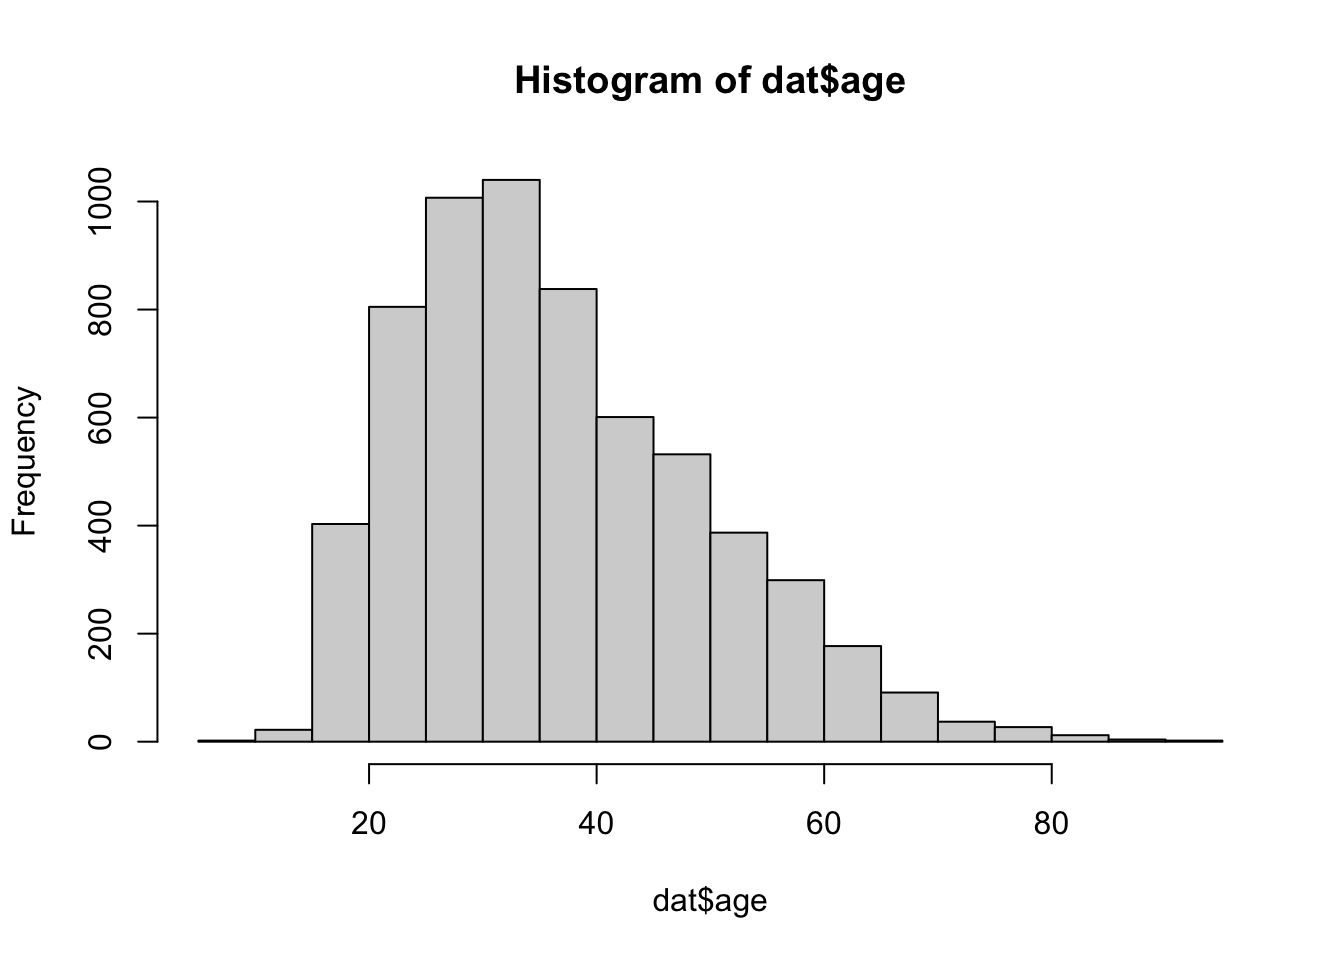
\includegraphics{Assignments_files/figure-latex/unnamed-chunk-34-1.pdf}

\begin{Shaded}
\begin{Highlighting}[]
\FunctionTok{summary}\NormalTok{(dat}\SpecialCharTok{$}\NormalTok{age)}
\end{Highlighting}
\end{Shaded}

\begin{verbatim}
##    Min. 1st Qu.  Median    Mean 3rd Qu.    Max.    NA's 
##    6.00   27.00   35.00   37.12   45.00   91.00     308
\end{verbatim}

\textbf{The data is skewed to the right, meaning that most of the
victims were towards the younger side. There are less cases of older
victim and the peak age is between between 30 and 40. I expected the
spread of data, however the minimum and maximum values were very
surprising.}

\begin{enumerate}
\def\labelenumi{\alph{enumi}.}
\setcounter{enumi}{1}
\tightlist
\item
  To understand the center of the age distribution, would you use a mean
  or a median, and why? Find the one you picked.
\end{enumerate}

\begin{Shaded}
\begin{Highlighting}[]
\FunctionTok{hist}\NormalTok{(dat}\SpecialCharTok{$}\NormalTok{age)}
\end{Highlighting}
\end{Shaded}

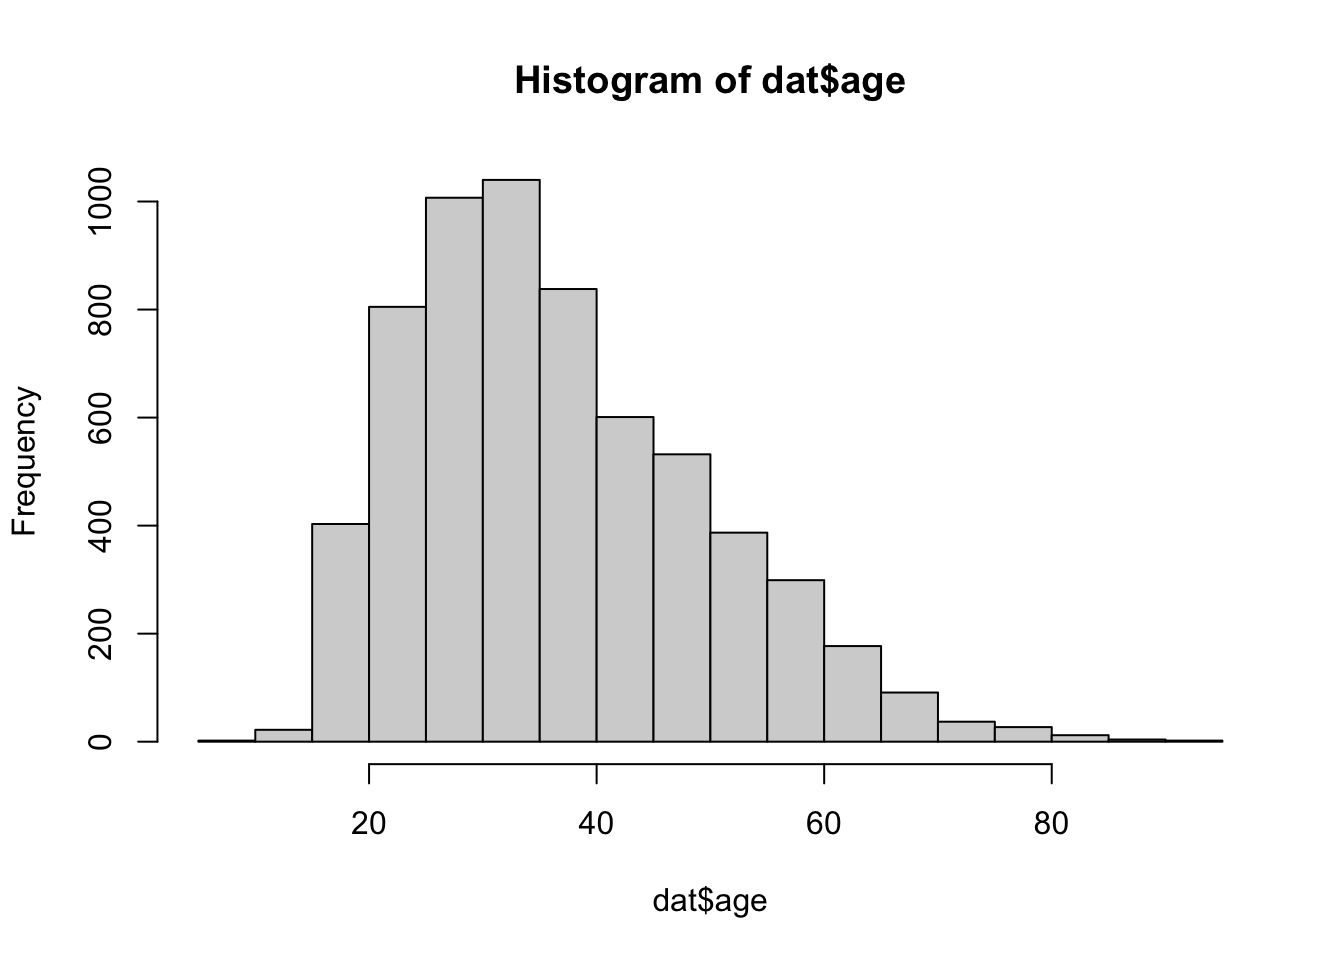
\includegraphics{Assignments_files/figure-latex/unnamed-chunk-35-1.pdf}

\begin{Shaded}
\begin{Highlighting}[]
\FunctionTok{summary}\NormalTok{(dat}\SpecialCharTok{$}\NormalTok{age)}
\end{Highlighting}
\end{Shaded}

\begin{verbatim}
##    Min. 1st Qu.  Median    Mean 3rd Qu.    Max.    NA's 
##    6.00   27.00   35.00   37.12   45.00   91.00     308
\end{verbatim}

\textbf{I would use the median because the center of distribution is the
median whereas the mean is the average of all the data points. The
median is 35.00. There are some missing values, but since they are not
assigned numeric values, they don't affect any analysis of my data, such
as finding the median. }

\begin{enumerate}
\def\labelenumi{\alph{enumi}.}
\setcounter{enumi}{2}
\tightlist
\item
  Describe the gender distribution of the sample. Do you find this
  surprising?
\end{enumerate}

\begin{Shaded}
\begin{Highlighting}[]
\FunctionTok{table}\NormalTok{(dat}\SpecialCharTok{$}\NormalTok{gender)}
\end{Highlighting}
\end{Shaded}

\begin{verbatim}
## 
##         F    M 
##    3  293 6298
\end{verbatim}

\begin{Shaded}
\begin{Highlighting}[]
\NormalTok{tab.gender }\OtherTok{\textless{}{-}} \FunctionTok{table}\NormalTok{(dat}\SpecialCharTok{$}\NormalTok{gender)}
\FunctionTok{barplot}\NormalTok{(tab.gender,}
        \AttributeTok{main =} \StringTok{"Stacked barchart"}\NormalTok{,}
        \AttributeTok{xlab =} \StringTok{"Gender"}\NormalTok{, }\AttributeTok{ylab =} \StringTok{"Frequency"}\NormalTok{,}
        \AttributeTok{legend.text =} \FunctionTok{rownames}\NormalTok{(tab.gender),}
        \AttributeTok{beside =} \ConstantTok{FALSE}\NormalTok{) }\CommentTok{\# Stacked bars (default)}
\end{Highlighting}
\end{Shaded}

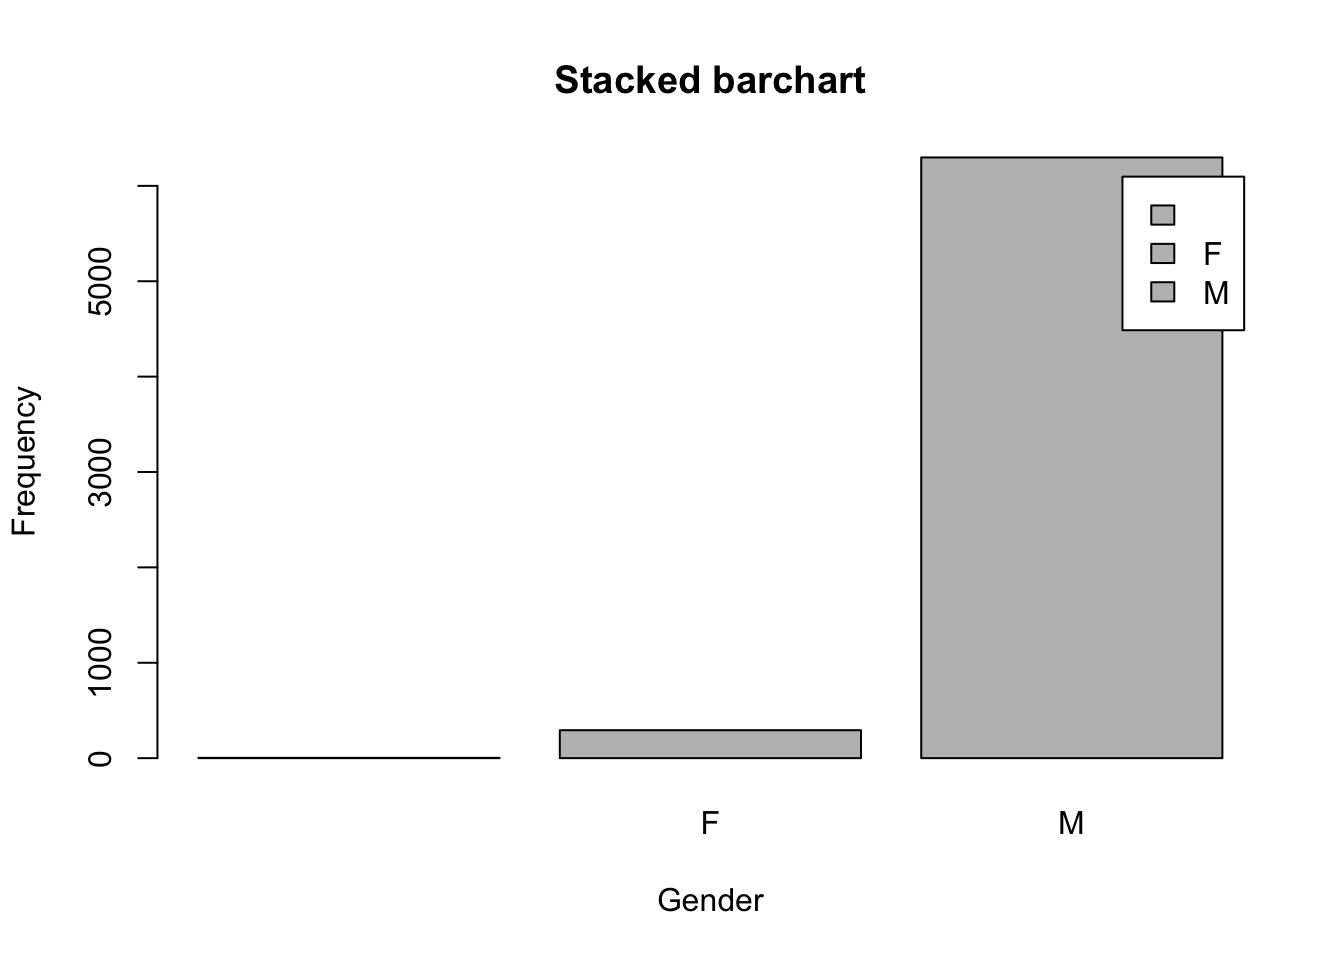
\includegraphics{Assignments_files/figure-latex/unnamed-chunk-36-1.pdf}

\textbf{There is about 21 times as much male victims as they are female
victims. It is important to note that there are also 3 missing values,
however not having these values do not impact the data because of how
many more male victims there are in comparison to female victims. I am
not surprised. I knew, before analyzing this data set, that men in the
US are shot to death by the police more than women. }

\hypertarget{problem-3-10-points}{%
\section{Problem 3 (10 points)}\label{problem-3-10-points}}

\begin{enumerate}
\def\labelenumi{\alph{enumi}.}
\tightlist
\item
  How many police officers had a body camera, according to news reports?
  What proportion is this of all the incidents in the data? Are you
  surprised that it is so high or low?
\end{enumerate}

\begin{Shaded}
\begin{Highlighting}[]
\FunctionTok{table}\NormalTok{(dat}\SpecialCharTok{$}\NormalTok{body\_camera)}
\end{Highlighting}
\end{Shaded}

\begin{verbatim}
## 
## False  True 
##  5684   910
\end{verbatim}

\textbf{910 police officers had a body camera, according to news
reports.This is 13.6 \% of all police officers. That is really
surprising! It seems that having a body camera would be a measure of
precaution for the officer that should be required, unless it is widely
acknowledged that police often kill civilians for no just reason and so
evidence on the body cameras would be damaging for the officers and
that's the reason why they are not required or at least not worn. }

\begin{enumerate}
\def\labelenumi{\alph{enumi}.}
\setcounter{enumi}{1}
\tightlist
\item
  In how many of the incidents was the victim fleeing? What proportion
  is this of the total number of incidents in the data? Is this what you
  would expect?
\end{enumerate}

\begin{Shaded}
\begin{Highlighting}[]
\FunctionTok{table}\NormalTok{(dat}\SpecialCharTok{$}\NormalTok{flee)}
\end{Highlighting}
\end{Shaded}

\begin{verbatim}
## 
##                     Car        Foot Not fleeing       Other 
##         491        1058         845        3952         248
\end{verbatim}

\begin{Shaded}
\begin{Highlighting}[]
\NormalTok{tab.flee }\OtherTok{\textless{}{-}} \FunctionTok{table}\NormalTok{(dat}\SpecialCharTok{$}\NormalTok{flee)}
\FunctionTok{barplot}\NormalTok{(tab.flee,}
        \AttributeTok{main =} \StringTok{"Barchart of Victims\textquotesingle{} Mode of Fleeing"}\NormalTok{,}
        \AttributeTok{xlab =} \StringTok{"Mode of Fleeing"}\NormalTok{, }\AttributeTok{ylab =} \StringTok{"Frequency"}\NormalTok{,}
        \AttributeTok{legend.text =} \FunctionTok{rownames}\NormalTok{(tab.flee),}
        \AttributeTok{beside =} \ConstantTok{FALSE}\NormalTok{) }\CommentTok{\# Stacked bars (default)}
\end{Highlighting}
\end{Shaded}

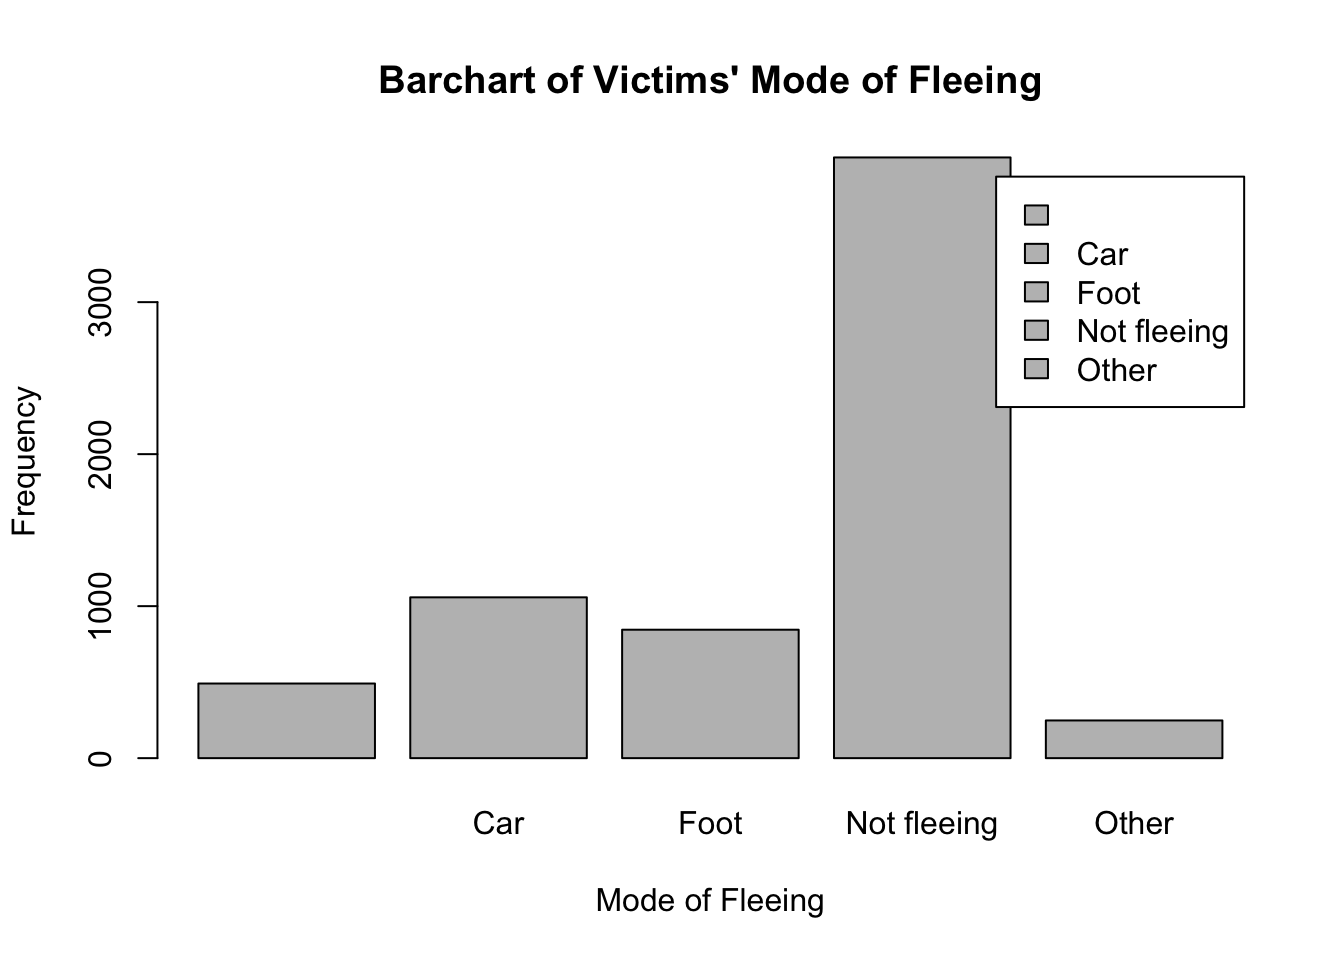
\includegraphics{Assignments_files/figure-latex/unnamed-chunk-38-1.pdf}

\textbf{The data is not very clear with the different modes of fleeing.
There are 248 cases that are categorized as ``other'' in terms of
fleeing. There are also 491 cases that have missing values. Therefore, I
will only consider those who fled by car or foot as fleeing and
disregard the cases categorized as missing or other. There are 1903
victims that fled and this is 28.9\% of all victims. I expected more
victims to have fled, but because there is such a great number of values
(the other and the missing) that aren't included, I don't really trust
this data's records of the number of victims who fled.}

\hypertarget{problem-4-10-points---answer-only-one-of-these-a-or-b.}{%
\section{Problem 4 (10 points) - Answer only one of these (a or
b).}\label{problem-4-10-points---answer-only-one-of-these-a-or-b.}}

\begin{enumerate}
\def\labelenumi{\alph{enumi}.}
\tightlist
\item
  Describe the relationship between the variables ``body camera'' and
  ``flee'' using a stacked barplot. What can you conclude from this
  relationship?
\end{enumerate}

\emph{Hint 1: The categories along the x-axis are the options for
``flee'', each bar contains information about whether the police officer
had a body camera (vertically), and the height along the y-axis shows
the frequency of that category).}

\emph{Hint 2: Also, if you are unsure about the syntax for barplot, run
?barplot in R and see some examples at the bottom of the documentation.
This is usually a good way to look up the syntax of R code. You can also
Google it.}

\textbf{Your answer here.}

\begin{enumerate}
\def\labelenumi{\alph{enumi}.}
\setcounter{enumi}{1}
\tightlist
\item
  Describe the relationship between age and race by using a boxplot.
  What can you conclude from this relationship?
\end{enumerate}

\emph{Hint 1: The categories along the x-axis are the race categories
and the height along the y-axis is age.}

\emph{Hint 2: Also, if you are unsure about the syntax for boxplot, run
?boxplot in R and see some examples at the bottom of the documentation.
This is usually a good way to look up the syntax of R code. You can also
Google it.}

\begin{Shaded}
\begin{Highlighting}[]
\FunctionTok{table}\NormalTok{(dat}\SpecialCharTok{$}\NormalTok{race,dat}\SpecialCharTok{$}\NormalTok{age)}
\end{Highlighting}
\end{Shaded}

\begin{verbatim}
##    
##       6  12  13  14  15  16  17  18  19  20  21  22  23  24  25  26  27  28  29
##       0   0   0   0   1   3   0   2   2   4   6  11   9   7  11  14  17  13  14
##   A   0   0   0   0   1   3   0   3   2   2   2   2   1   0   3   4   3   4   1
##   B   0   0   1   0   6  11  24  50  45  41  54  45  56  69  76  39  69  59  57
##   H   0   0   1   2   5   8  12  25  18  19  31  38  27  34  37  40  44  44  41
##   N   0   0   0   1   0   0   0   1   3   2   2   1   2   5   5   3   8   4   3
##   O   0   0   0   0   0   0   0   3   0   2   0   2   1   1   3   1   4   1   4
##   W   2   1   0   0   3  10  20  25  28  35  29  39  52  63  81  87  72  69  84
##    
##      30  31  32  33  34  35  36  37  38  39  40  41  42  43  44  45  46  47  48
##      20  22  16  14  13  19  12  11  13  16  17  10  10  13   8  10  14   9  16
##   A   2   2   4   4   4   7   3   2   5   2   1   2   2   1   3   3   1   2   2
##   B  52  69  53  53  44  43  34  51  31  46  24  32  19  22  14  19  19  25  20
##   H  32  33  34  38  41  39  34  45  39  29  23  23  19  12  18  20  18  16   9
##   N   4   2   6   3   4   4   4   2   1   2   1   1   1   4   2   1   1   0   0
##   O   4   1   1   1   2   0   2   0   2   0   1   1   1   0   0   1   1   0   2
##   W  90  94  93  92 101  84  97  72  73  70  73  73  60  68  56  72  55  63  61
##    
##      49  50  51  52  53  54  55  56  57  58  59  60  61  62  63  64  65  66  67
##      15   7   7  12  12  14   9   8   5   2  12   4   5   7   8   5   7   2   4
##   A   2   2   1   2   3   1   2   1   0   0   1   3   1   1   0   0   0   0   0
##   B  17  11  10  12   9   8  12   6  11   3   2   7  10   5   6   2   2   2   5
##   H  10  16   9  13   3   3  10   3   7   5   4   2   1   3   2   1   3   1   0
##   N   2   1   1   0   1   1   0   0   0   1   0   0   0   0   0   0   0   0   0
##   O   0   0   1   0   0   1   0   1   0   0   1   0   0   0   0   0   0   0   0
##   W  57  58  60  43  50  43  34  53  35  45  46  31  27  29  19  17  16  14  14
##    
##      68  69  70  71  72  73  74  75  76  77  78  79  80  81  82  83  84  86  88
##       2   2   3   3   2   3   1   1   3   2   0   0   3   1   0   1   0   2   0
##   A   0   0   0   0   0   0   0   0   0   0   0   0   0   0   0   0   0   0   0
##   B   5   1   1   0   1   0   2   0   0   1   0   0   0   0   0   0   0   0   1
##   H   0   3   3   2   0   1   0   0   0   0   0   0   1   0   0   0   0   0   0
##   N   0   0   0   0   0   0   0   0   0   0   0   0   0   0   0   0   0   0   0
##   O   0   0   0   0   0   0   0   0   0   0   0   0   0   0   0   0   0   0   0
##   W   9  11   9   7   4   3   3   4   9   2   1   4   1   2   2   2   4   0   0
##    
##      89  91
##       1   0
##   A   0   0
##   B   0   0
##   H   0   0
##   N   0   0
##   O   0   0
##   W   0   2
\end{verbatim}

\begin{Shaded}
\begin{Highlighting}[]
\NormalTok{tab.raceage }\OtherTok{\textless{}{-}} \FunctionTok{table}\NormalTok{(dat}\SpecialCharTok{$}\NormalTok{race,dat}\SpecialCharTok{$}\NormalTok{age)}
\FunctionTok{barplot}\NormalTok{(tab.raceage,}
        \AttributeTok{main =} \StringTok{"Barchart of Age and Race"}\NormalTok{,}
        \AttributeTok{xlab =} \StringTok{"Race Categories"}\NormalTok{, }\AttributeTok{ylab =} \StringTok{"Age"}\NormalTok{,}
        \AttributeTok{legend.text =} \FunctionTok{rownames}\NormalTok{(tab.raceage),}
        \AttributeTok{beside =} \ConstantTok{FALSE}\NormalTok{) }\CommentTok{\# Stacked bars (default)}
\end{Highlighting}
\end{Shaded}

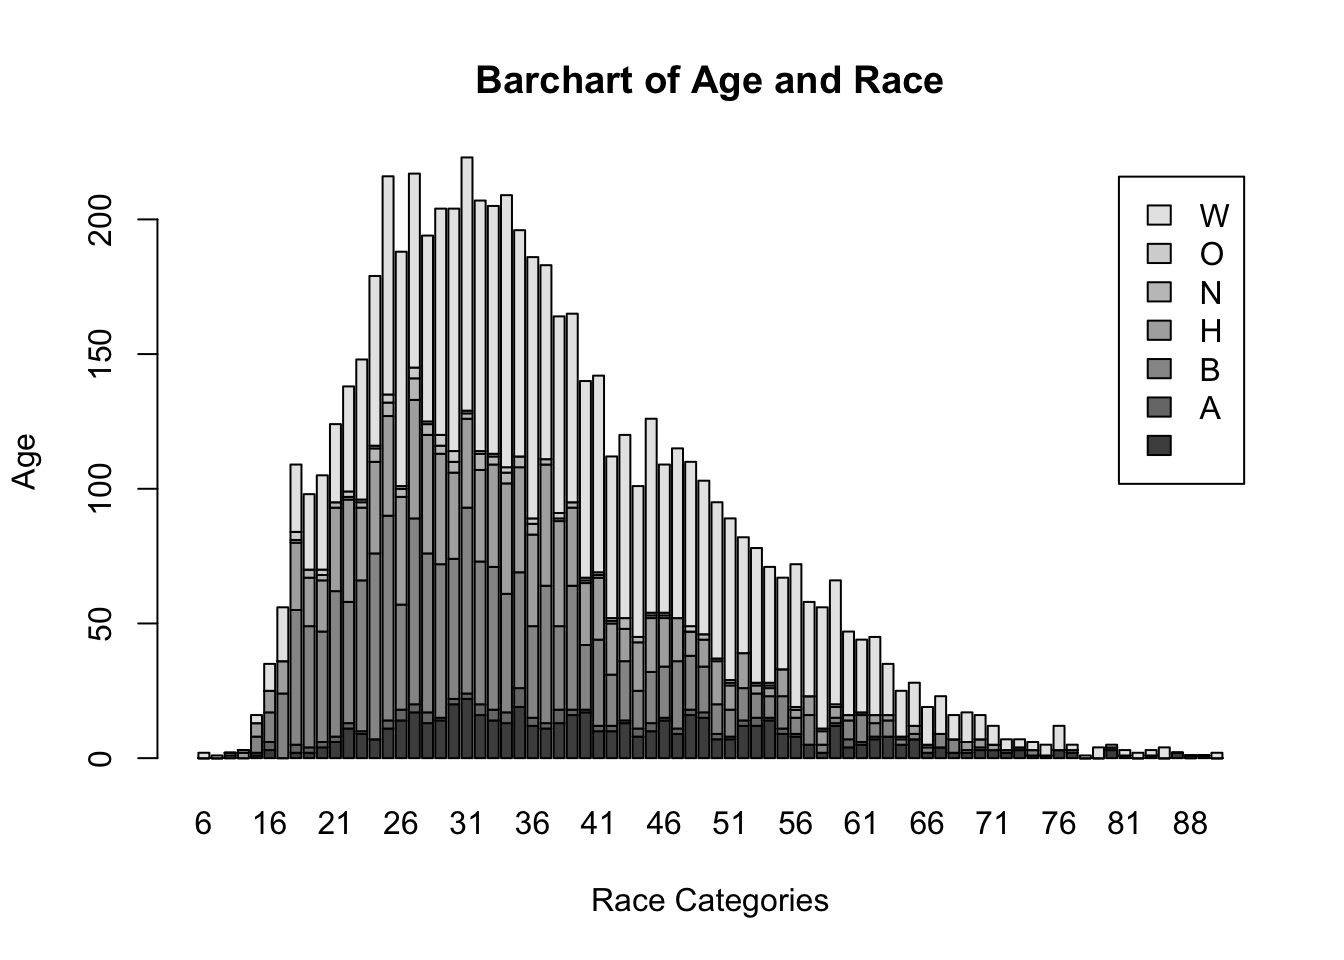
\includegraphics{Assignments_files/figure-latex/unnamed-chunk-40-1.pdf}

\begin{Shaded}
\begin{Highlighting}[]
\FunctionTok{table}\NormalTok{(dat}\SpecialCharTok{$}\NormalTok{age,dat}\SpecialCharTok{$}\NormalTok{race)}
\end{Highlighting}
\end{Shaded}

\begin{verbatim}
##     
##            A   B   H   N   O   W
##   6    0   0   0   0   0   0   2
##   12   0   0   0   0   0   0   1
##   13   0   0   1   1   0   0   0
##   14   0   0   0   2   1   0   0
##   15   1   1   6   5   0   0   3
##   16   3   3  11   8   0   0  10
##   17   0   0  24  12   0   0  20
##   18   2   3  50  25   1   3  25
##   19   2   2  45  18   3   0  28
##   20   4   2  41  19   2   2  35
##   21   6   2  54  31   2   0  29
##   22  11   2  45  38   1   2  39
##   23   9   1  56  27   2   1  52
##   24   7   0  69  34   5   1  63
##   25  11   3  76  37   5   3  81
##   26  14   4  39  40   3   1  87
##   27  17   3  69  44   8   4  72
##   28  13   4  59  44   4   1  69
##   29  14   1  57  41   3   4  84
##   30  20   2  52  32   4   4  90
##   31  22   2  69  33   2   1  94
##   32  16   4  53  34   6   1  93
##   33  14   4  53  38   3   1  92
##   34  13   4  44  41   4   2 101
##   35  19   7  43  39   4   0  84
##   36  12   3  34  34   4   2  97
##   37  11   2  51  45   2   0  72
##   38  13   5  31  39   1   2  73
##   39  16   2  46  29   2   0  70
##   40  17   1  24  23   1   1  73
##   41  10   2  32  23   1   1  73
##   42  10   2  19  19   1   1  60
##   43  13   1  22  12   4   0  68
##   44   8   3  14  18   2   0  56
##   45  10   3  19  20   1   1  72
##   46  14   1  19  18   1   1  55
##   47   9   2  25  16   0   0  63
##   48  16   2  20   9   0   2  61
##   49  15   2  17  10   2   0  57
##   50   7   2  11  16   1   0  58
##   51   7   1  10   9   1   1  60
##   52  12   2  12  13   0   0  43
##   53  12   3   9   3   1   0  50
##   54  14   1   8   3   1   1  43
##   55   9   2  12  10   0   0  34
##   56   8   1   6   3   0   1  53
##   57   5   0  11   7   0   0  35
##   58   2   0   3   5   1   0  45
##   59  12   1   2   4   0   1  46
##   60   4   3   7   2   0   0  31
##   61   5   1  10   1   0   0  27
##   62   7   1   5   3   0   0  29
##   63   8   0   6   2   0   0  19
##   64   5   0   2   1   0   0  17
##   65   7   0   2   3   0   0  16
##   66   2   0   2   1   0   0  14
##   67   4   0   5   0   0   0  14
##   68   2   0   5   0   0   0   9
##   69   2   0   1   3   0   0  11
##   70   3   0   1   3   0   0   9
##   71   3   0   0   2   0   0   7
##   72   2   0   1   0   0   0   4
##   73   3   0   0   1   0   0   3
##   74   1   0   2   0   0   0   3
##   75   1   0   0   0   0   0   4
##   76   3   0   0   0   0   0   9
##   77   2   0   1   0   0   0   2
##   78   0   0   0   0   0   0   1
##   79   0   0   0   0   0   0   4
##   80   3   0   0   1   0   0   1
##   81   1   0   0   0   0   0   2
##   82   0   0   0   0   0   0   2
##   83   1   0   0   0   0   0   2
##   84   0   0   0   0   0   0   4
##   86   2   0   0   0   0   0   0
##   88   0   0   1   0   0   0   0
##   89   1   0   0   0   0   0   0
##   91   0   0   0   0   0   0   2
\end{verbatim}

\begin{Shaded}
\begin{Highlighting}[]
\NormalTok{tab.raceage }\OtherTok{\textless{}{-}} \FunctionTok{table}\NormalTok{(dat}\SpecialCharTok{$}\NormalTok{age,dat}\SpecialCharTok{$}\NormalTok{race)}
\FunctionTok{barplot}\NormalTok{(tab.raceage,}
        \AttributeTok{main =} \StringTok{"Barchart of Age and Race"}\NormalTok{,}
        \AttributeTok{xlab =} \StringTok{"Race Categories"}\NormalTok{, }\AttributeTok{ylab =} \StringTok{"Age"}\NormalTok{,}
        \AttributeTok{legend.text =} \FunctionTok{rownames}\NormalTok{(tab.raceage),}
        \AttributeTok{beside =} \ConstantTok{FALSE}\NormalTok{) }\CommentTok{\# Stacked bars (default)}
\end{Highlighting}
\end{Shaded}

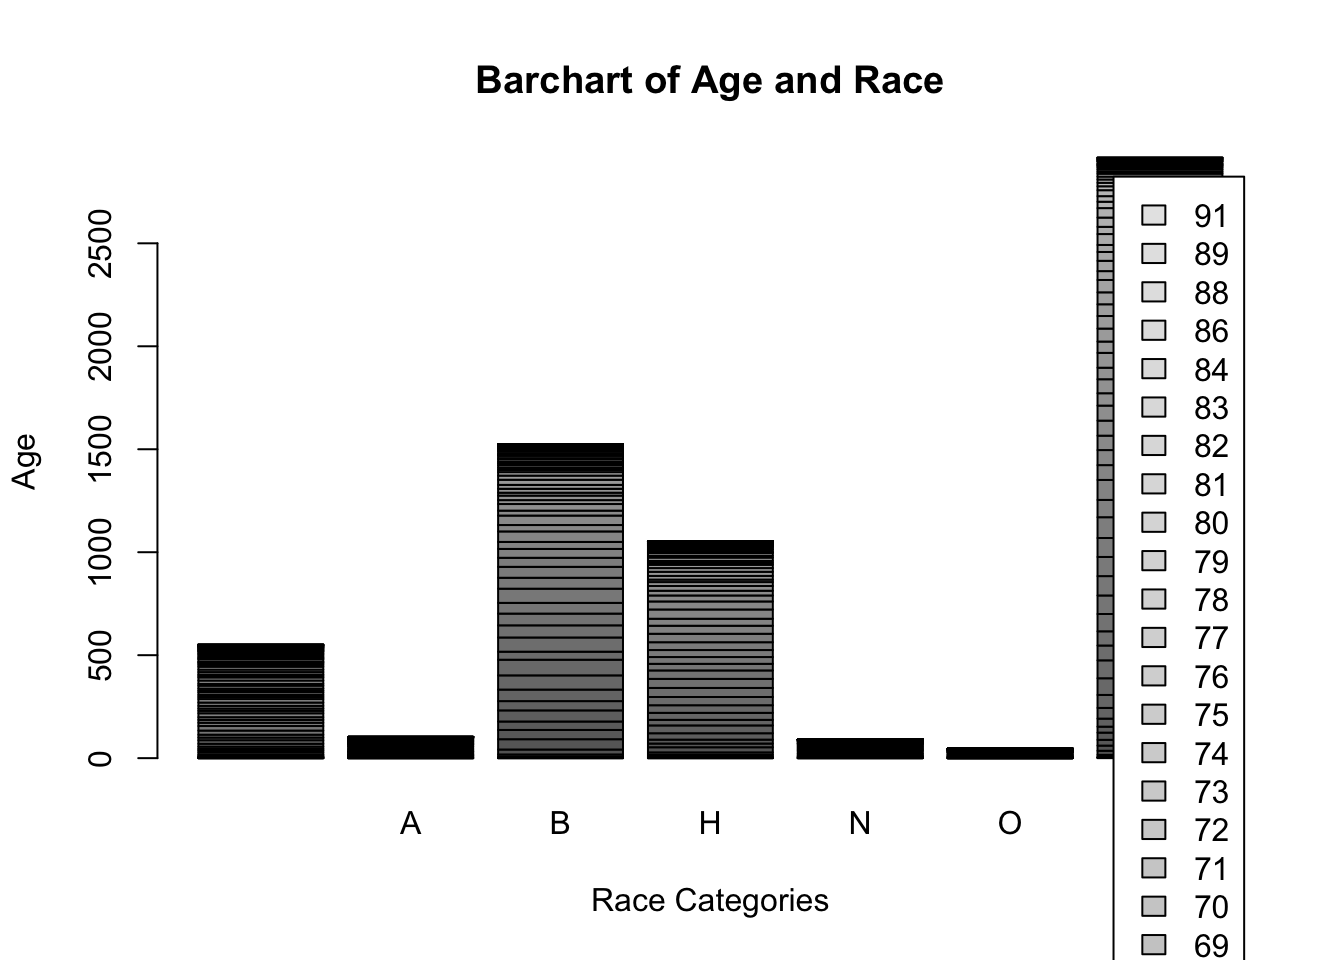
\includegraphics{Assignments_files/figure-latex/unnamed-chunk-41-1.pdf}
\textbf{Disregard first histogram. THere is a great number of older
black and hispanic victims. There is also a great deal of victims whose
races are not clarified, which is problematic in making a conclusion of
the types of victims that are killed at the hands of police. White males
however represent the group with the oldest victims killed by police. }

\hypertarget{extra-credit-10-points}{%
\section{Extra credit (10 points)}\label{extra-credit-10-points}}

\begin{enumerate}
\def\labelenumi{\alph{enumi}.}
\tightlist
\item
  What does this code tell us?
\end{enumerate}

\begin{Shaded}
\begin{Highlighting}[]
\NormalTok{mydates }\OtherTok{\textless{}{-}} \FunctionTok{as.Date}\NormalTok{(dat}\SpecialCharTok{$}\NormalTok{date)}
\FunctionTok{head}\NormalTok{(mydates)}
\NormalTok{(mydates[}\FunctionTok{length}\NormalTok{(mydates)] }\SpecialCharTok{{-}}\NormalTok{ mydates[}\DecValTok{1}\NormalTok{])}
\end{Highlighting}
\end{Shaded}

\begin{enumerate}
\def\labelenumi{\alph{enumi}.}
\setcounter{enumi}{1}
\item
  On Friday, a new report was published that was described as follows by
  The Guardian: ``More than half of US police killings are mislabelled
  or not reported, study finds.'' Without reading this article now (due
  to limited time), why do you think police killings might be
  mislabelled or underreported?
\item
  Regarding missing values in problem 4, do you see any? If so, do you
  think that's all that's missing from the data?
\end{enumerate}

This code arranges my data into the dates during which the cases
occured.The last line of the code tells us the time difference. They
might be mislabelled or underreported because so much of the data in
this data set are either missing or unclear so that you can't make clear
conclusions of the rate of police killings. There are missing data
points in problem 4, however I don't think that's all that is missing,
if the rest of the data frame is any indication.

\hypertarget{exam-2}{%
\section{Exam 2}\label{exam-2}}

\hypertarget{instructions-1}{%
\section{Instructions}\label{instructions-1}}

\begin{enumerate}
\def\labelenumi{\alph{enumi}.}
\item
  Create a folder in your computer (a good place would be under Crim
  250, Exams).
\item
  Download the dataset from the Canvas website (sim.data.csv) onto that
  folder, and save your Exam 2.Rmd file in the same folder.
\item
  Data description: This dataset provides (simulated) data about 200
  police departments in one year. It contains information about the
  funding received by the department as well as incidents of police
  brutality. Suppose this dataset (sim.data.csv) was collected by
  researchers to answer this question: \textbf{``Does having more
  funding in a police department lead to fewer incidents of police
  brutality?''}
\item
  Codebook:
\end{enumerate}

\begin{itemize}
\tightlist
\item
  funds: How much funding the police department received in that year in
  millions of dollars.
\item
  po.brut: How many incidents of police brutality were reported by the
  department that year.
\item
  po.dept.code: Police department code
\end{itemize}

\hypertarget{problem-1-eda-10-points}{%
\section{Problem 1: EDA (10 points)}\label{problem-1-eda-10-points}}

Describe the dataset and variables. Perform exploratory data analysis
for the two variables of interest: funds and po.brut.

\begin{Shaded}
\begin{Highlighting}[]
\NormalTok{dat }\OtherTok{\textless{}{-}} \FunctionTok{read.csv}\NormalTok{(}\AttributeTok{file =} \StringTok{\textquotesingle{}sim.data.csv\textquotesingle{}}\NormalTok{)}
\FunctionTok{class}\NormalTok{(dat}\SpecialCharTok{$}\NormalTok{funds)}
\end{Highlighting}
\end{Shaded}

\begin{verbatim}
## [1] "numeric"
\end{verbatim}

\begin{Shaded}
\begin{Highlighting}[]
\FunctionTok{class}\NormalTok{ (dat}\SpecialCharTok{$}\NormalTok{po.dept.code)}
\end{Highlighting}
\end{Shaded}

\begin{verbatim}
## [1] "integer"
\end{verbatim}

\begin{Shaded}
\begin{Highlighting}[]
\FunctionTok{class}\NormalTok{ (dat}\SpecialCharTok{$}\NormalTok{po.brut)}
\end{Highlighting}
\end{Shaded}

\begin{verbatim}
## [1] "integer"
\end{verbatim}

\begin{Shaded}
\begin{Highlighting}[]
\NormalTok{table}\OtherTok{\textless{}{-}}\FunctionTok{table}\NormalTok{ (dat}\SpecialCharTok{$}\NormalTok{funds,dat}\SpecialCharTok{$}\NormalTok{po.brut)}
\end{Highlighting}
\end{Shaded}

```\{\{r, fig.width=4, fig.height=4\} x \textless-
dat\(funds y <- dat\)po.brut plot(x, y, main = ``Scatterplot of Funding
for Police Departments Vs. Number of Instances of Police Brutality'',
xlab = ``Funding for Police Departments (in millions)'', ylab = ``Number
of Instances of Police Brutality'', pch = 19, frame = FALSE) cor(x, y,
method = c(``pearson'', ``kendall'', ``spearman'')) abline(reg.output,
col = ``red'', lwd=2)

barplot(table, main = ``Barchart of Funding for Police Departments Vs.
Number of Instances of Police Brutality'', xlab = ``Funding for Police
Departments (in millions)'', ylab = ``Number of Instances of Police
Brutality'', legend.text = rownames(table), beside = FALSE)

\begin{verbatim}
__The data set, which observes the instances of police brutality across 200 police departments,  is comprised of 200 observations of 3 variables, the variables being funds, po. brut, and po.dept.code.  Funds is a quantitative variable with units millions of dollars, brut is a quantitative variable, and po.dept. code is an identifier variable. In terms of r, funds is a numeric variable while po.brut an po.dept.code are integers. Since I have two continuous, qualitative variables, I first created a table  since it is the most basic bivariate non-graphical technique of EDA, however it was difficult to contextualize the data with just the table. Therefore, I made a barchart and a scatter plot. The barchart was not as reliable in analyzing the data as the frequency of instances of police bruatity continued to fluctuate as the funding increased. However, the scatterplot suggested (with a very strong negative correlation) that the more funds a department receives, the less instances of police brutality occurs. In the steps below, I realize this conclusion I've made is not actually accurate. __


# Problem 2: Linear regression (30 points)

a. Perform a simple linear regression to answer the question of interest. To do this, name your linear model "reg.output" and write the summary of the regression by using "summary(reg.output)". 


```r
# Remember to remove eval=FALSE!!
reg.output <- lm(formula = po.brut ~ funds, data = dat)
summary(reg.output)
\end{verbatim}

\begin{verbatim}
## 
## Call:
## lm(formula = po.brut ~ funds, data = dat)
## 
## Residuals:
##     Min      1Q  Median      3Q     Max 
## -3.9433 -0.2233  0.2544  0.5952  1.1803 
## 
## Coefficients:
##              Estimate Std. Error t value Pr(>|t|)    
## (Intercept) 40.543069   0.282503  143.51   <2e-16 ***
## funds       -0.367099   0.004496  -81.64   <2e-16 ***
## ---
## Signif. codes:  0 '***' 0.001 '**' 0.01 '*' 0.05 '.' 0.1 ' ' 1
## 
## Residual standard error: 0.9464 on 198 degrees of freedom
## Multiple R-squared:  0.9712, Adjusted R-squared:  0.971 
## F-statistic:  6666 on 1 and 198 DF,  p-value: < 2.2e-16
\end{verbatim}

\textbf{According to the linear regression model, having more funding in
the police departments does not lead to fewer instances of police
bruatlity. The summary shows that the Pr(\textgreater\textbar t\textbar)
value of \textless2e-16 is 0\% statistically significant.}

\begin{enumerate}
\def\labelenumi{\alph{enumi}.}
\setcounter{enumi}{1}
\tightlist
\item
  Report the estimated coefficient, standard error, and p-value of the
  slope. Is the relationship between funds and incidents statistically
  significant? Explain.
\end{enumerate}

\textbf{The estimated coefficient = -0.367099, the standard error =
0.004496, and the p value of the slope = \textless2e-16. According to
the summary, the relationship between funds and incidents is not
statistically significant. Typically, when the p value is less than or
equal to the significance level (p = 0.05), we can reject the null
hypothesis, meaning there is a definite consequential relationship
between the two variables. The p value here was so low indicating that
null hypothesis is very incompatible with the dta collected. This leads
me to beleive that the two variables have too many other factors in play
that a correlation between just funding and instances of police
brutality would be oversimplifying the issue. .}

\begin{enumerate}
\def\labelenumi{\alph{enumi}.}
\setcounter{enumi}{2}
\tightlist
\item
  Draw a scatterplot of po.brut (y-axis) and funds (x-axis). Right below
  your plot command, use abline to draw the fitted regression line, like
  this:
\end{enumerate}

\hypertarget{remember-to-remove-evalfalse}{%
\section{Remember to remove
eval=FALSE!!}\label{remember-to-remove-evalfalse}}

\texttt{\{\{r,\ fig.width=4,\ fig.height=4\}\ x\ \textless{}-\ dat\$funds\ \ y\ \textless{}-\ dat\$po.brut\ plot(x,\ y,\ main\ =\ "Scatterplot\ of\ Funding\ for\ Police\ Departments\ Vs.\ Number\ of\ Instances\ of\ Police\ Brutality",\ \ \ \ \ \ xlab\ =\ "Funding\ for\ Police\ Departments\ (in\ millions)",\ ylab\ =\ "Number\ of\ Instances\ of\ Police\ Brutality",\ \ \ \ \ \ pch\ =\ 19,\ frame\ =\ FALSE)\ cor(x,\ y,\ method\ =\ c("pearson",\ "kendall",\ "spearman"))\ abline(reg.output,\ col\ =\ "red",\ lwd=2)}

Does the line look like a good fit? Why or why not?

\textbf{The line passes through most of the data points, especially in
the center of the graph. Thus, it appears to be a good fit.}

\begin{enumerate}
\def\labelenumi{\alph{enumi}.}
\setcounter{enumi}{3}
\tightlist
\item
  Are the four assumptions of linear regression satisfied? To answer
  this, draw the relevant plots. (Write a maximum of one sentence per
  assumption.) If not, what might you try to do to improve this (if you
  had more time)?
\end{enumerate}

\begin{Shaded}
\begin{Highlighting}[]
\FunctionTok{install.packages}\NormalTok{(}\StringTok{"ggplot2"}\NormalTok{,}\AttributeTok{repos =} \StringTok{"http://cran.us.r{-}project.org"}\NormalTok{)}
\end{Highlighting}
\end{Shaded}

\begin{verbatim}
## 
## The downloaded binary packages are in
##  /var/folders/nh/m2s_dxnj099clcww6tpc2vy00000gn/T//Rtmpa8F00e/downloaded_packages
\end{verbatim}

\begin{Shaded}
\begin{Highlighting}[]
\FunctionTok{install.packages}\NormalTok{(}\StringTok{"ggfortify"}\NormalTok{,}\AttributeTok{repos =} \StringTok{"http://cran.us.r{-}project.org"}\NormalTok{)}
\end{Highlighting}
\end{Shaded}

\begin{verbatim}
## 
## The downloaded binary packages are in
##  /var/folders/nh/m2s_dxnj099clcww6tpc2vy00000gn/T//Rtmpa8F00e/downloaded_packages
\end{verbatim}

\begin{Shaded}
\begin{Highlighting}[]
\FunctionTok{library}\NormalTok{ (ggplot2)}
\FunctionTok{library}\NormalTok{(ggfortify)}
\FunctionTok{autoplot}\NormalTok{(reg.output)}
\end{Highlighting}
\end{Shaded}

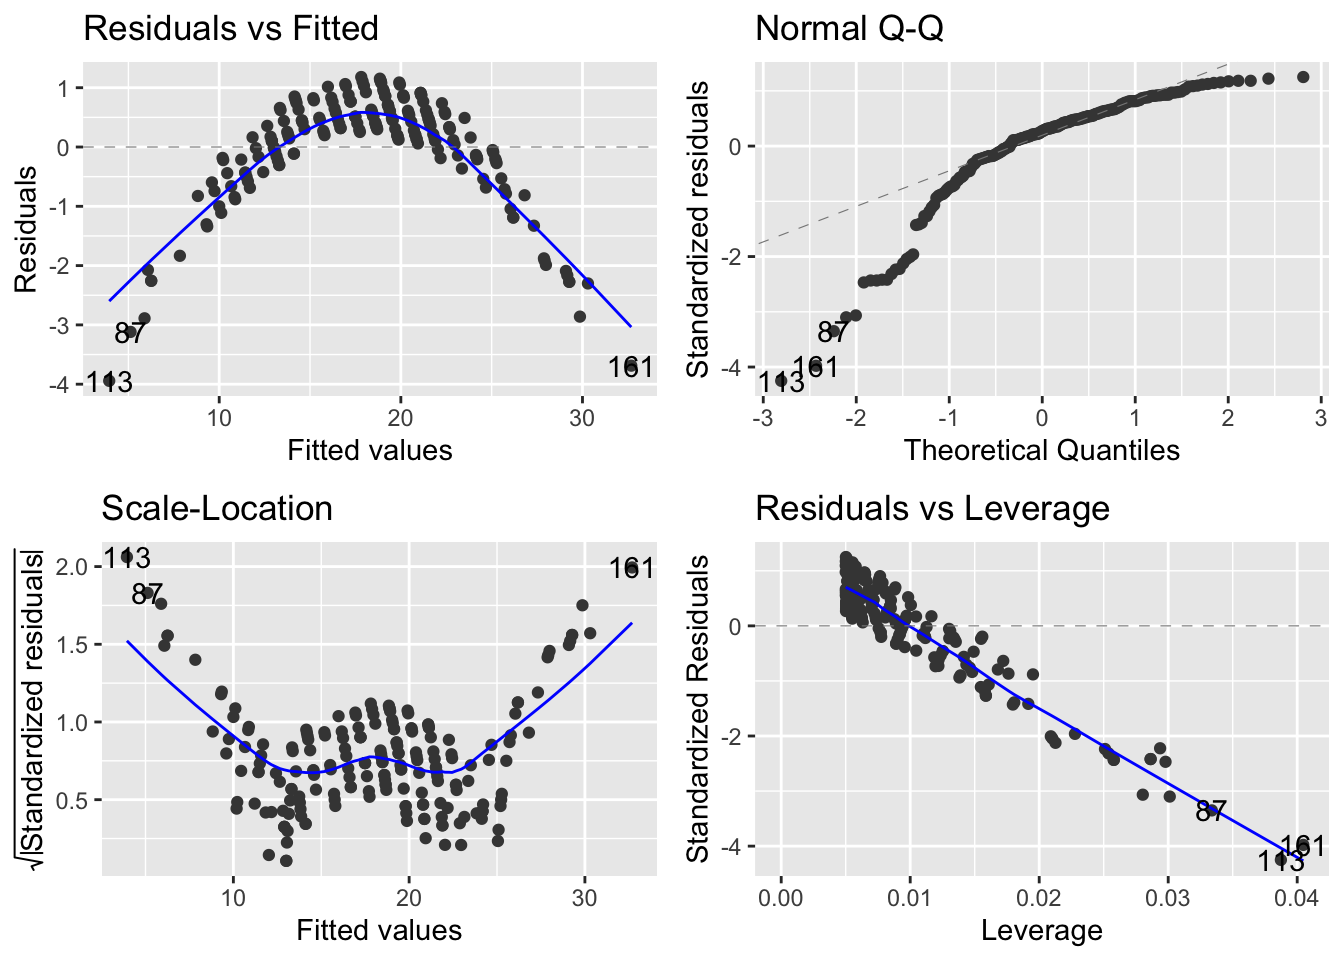
\includegraphics{Assignments_files/figure-latex/unnamed-chunk-45-1.pdf}

\begin{Shaded}
\begin{Highlighting}[]
\FunctionTok{plot}\NormalTok{(reg.output, }\DecValTok{1}\NormalTok{)}
\end{Highlighting}
\end{Shaded}

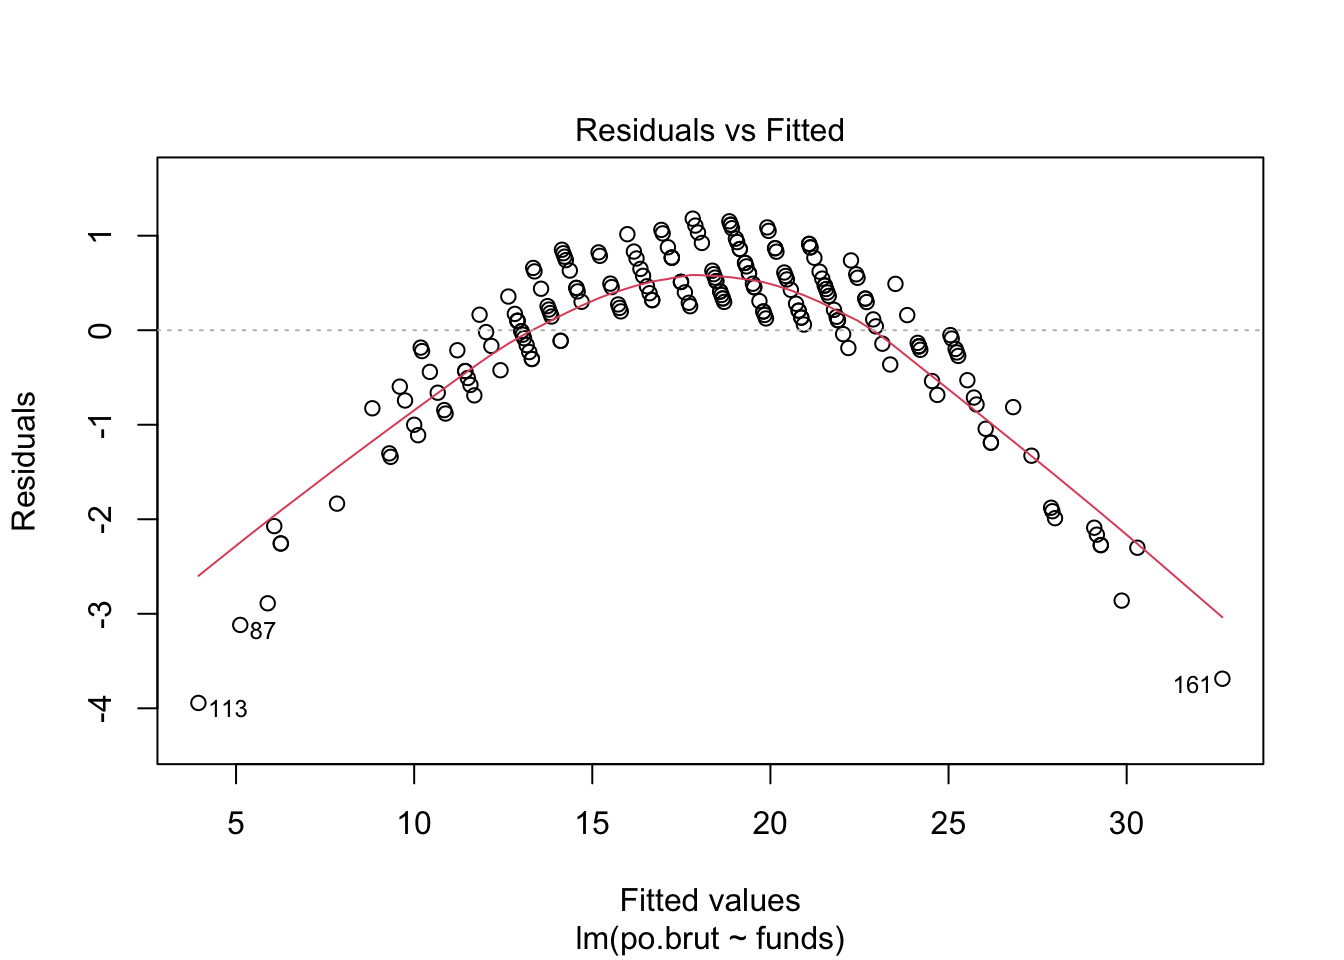
\includegraphics{Assignments_files/figure-latex/unnamed-chunk-45-2.pdf}

\begin{Shaded}
\begin{Highlighting}[]
\FunctionTok{plot}\NormalTok{(reg.output, }\DecValTok{3}\NormalTok{)}
\end{Highlighting}
\end{Shaded}

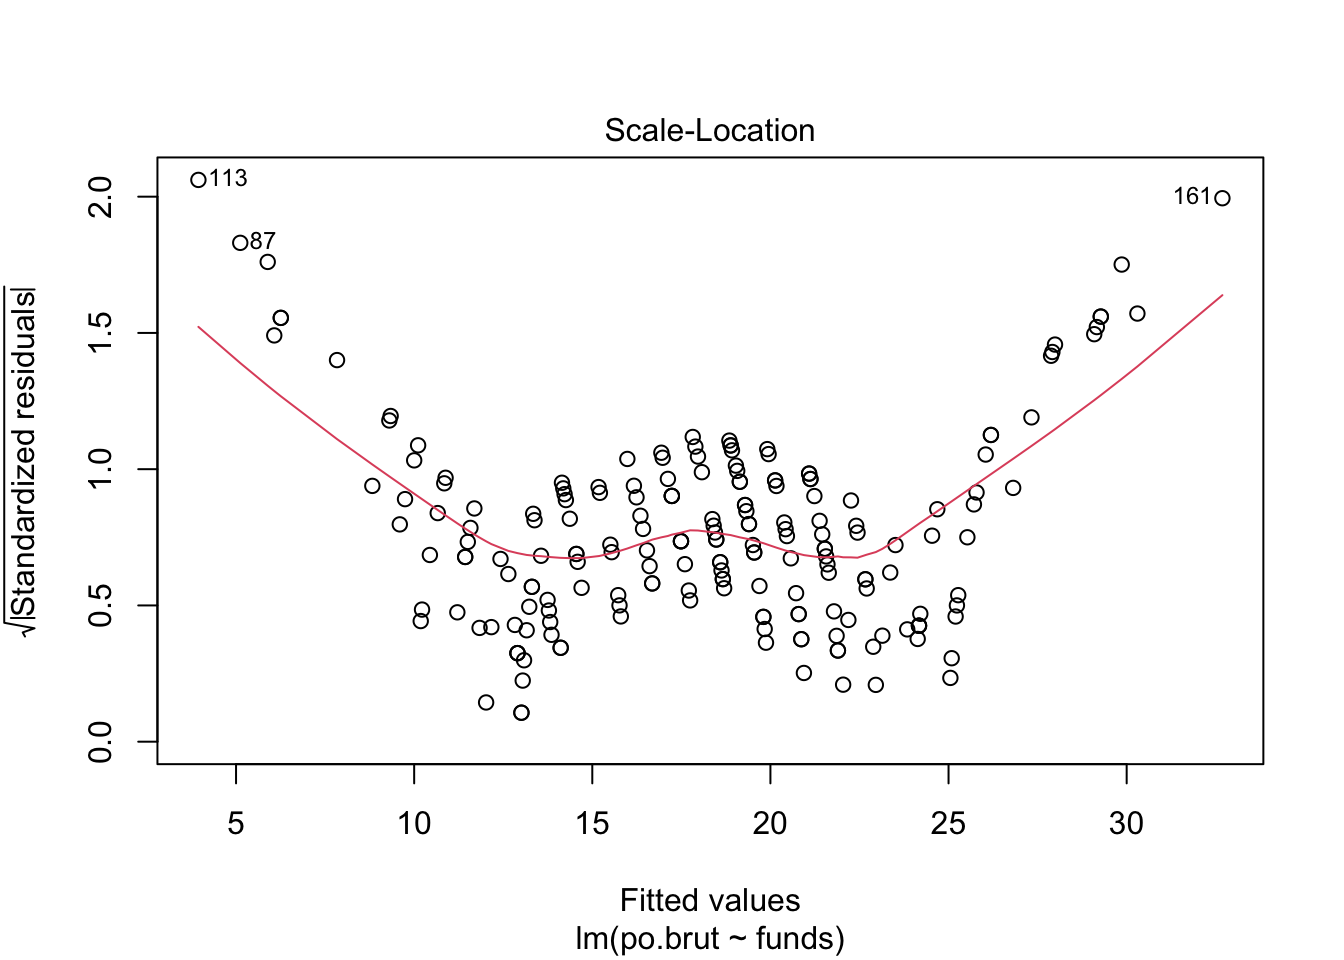
\includegraphics{Assignments_files/figure-latex/unnamed-chunk-45-3.pdf}

\begin{Shaded}
\begin{Highlighting}[]
\FunctionTok{plot}\NormalTok{(reg.output, }\DecValTok{2}\NormalTok{)}
\end{Highlighting}
\end{Shaded}

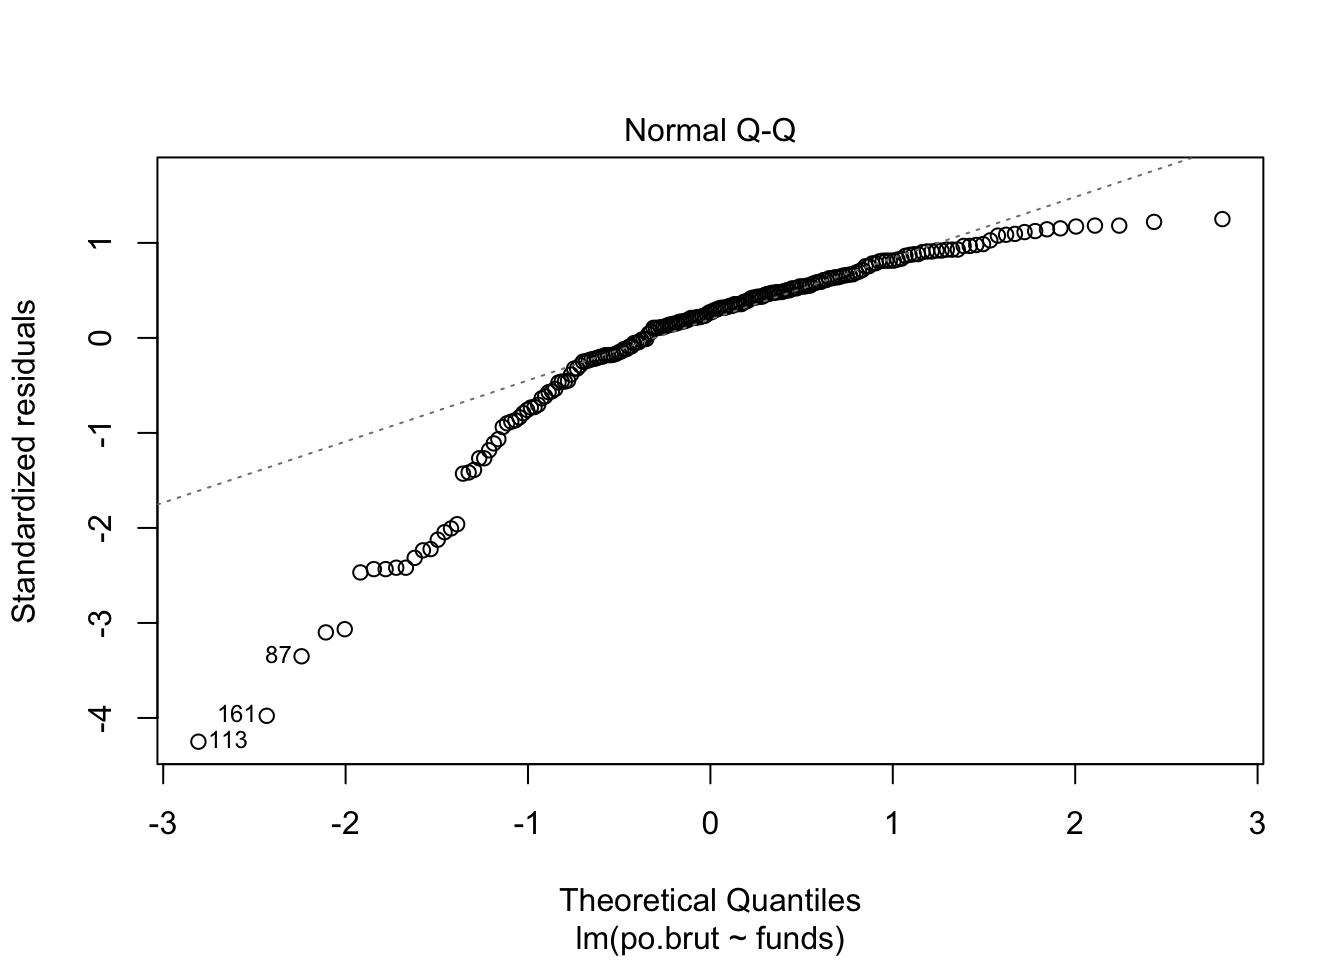
\includegraphics{Assignments_files/figure-latex/unnamed-chunk-45-4.pdf}

\begin{Shaded}
\begin{Highlighting}[]
\FunctionTok{plot}\NormalTok{(reg.output, }\DecValTok{5}\NormalTok{)}
\end{Highlighting}
\end{Shaded}

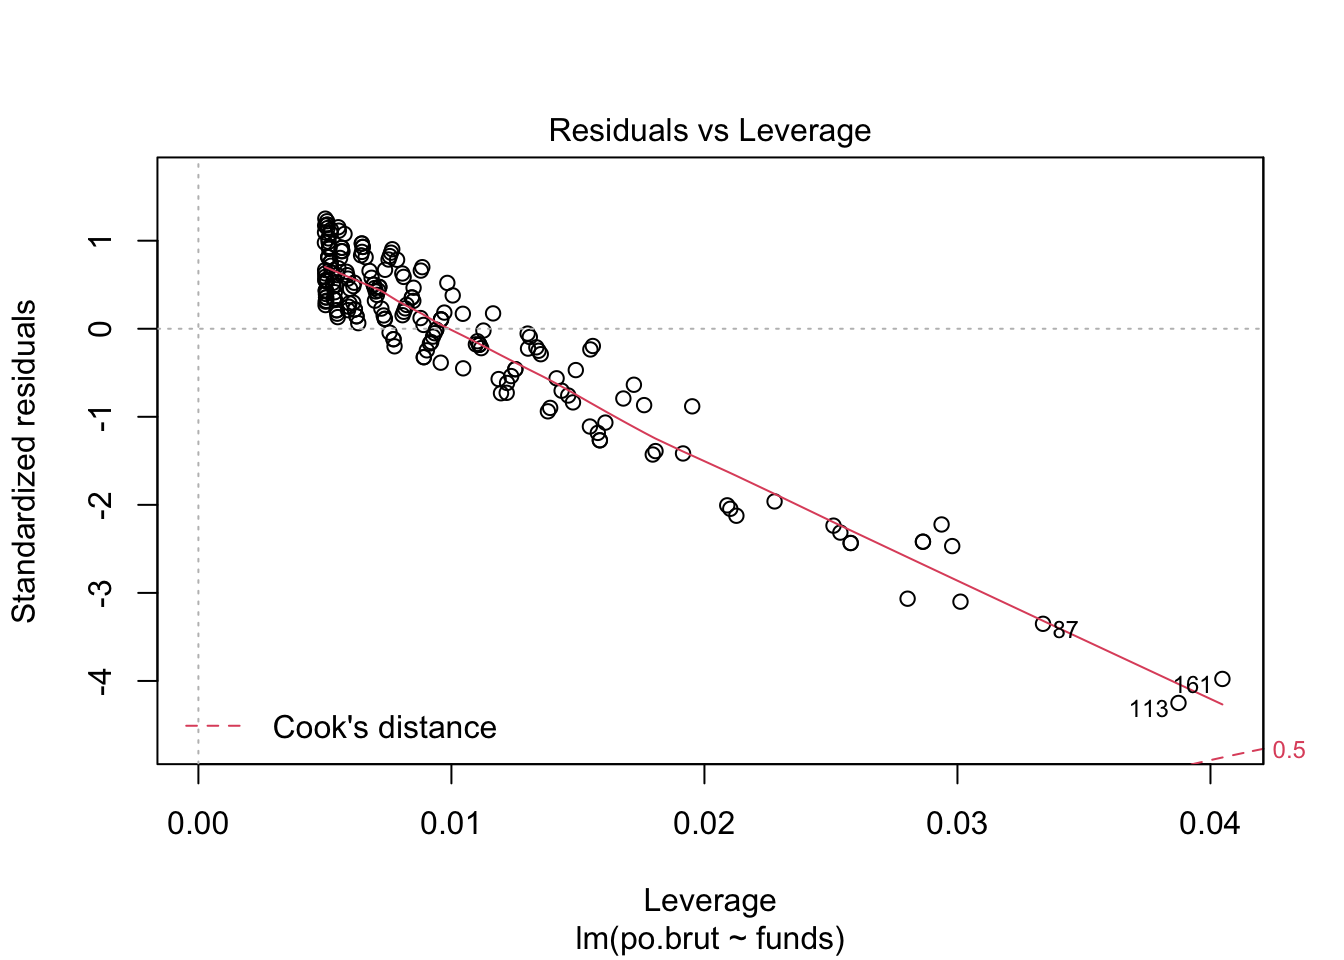
\includegraphics{Assignments_files/figure-latex/unnamed-chunk-45-5.pdf}

\textbf{The assumption of linearity is not satisfied because the
residual plot shows a fitted pattern, as in the red line is not at all
horizontal at zero. The assumption of homoscedasticity is not satisfied
because there isn't a horizontal line with equally spread points since
the variability of the residual points decreases, increases, decreases,
and finally increases as the value of the fitted outcome variable
increases, suggesting non-constant variances in the residuals errors (or
heteroscedasticity).The assumption of normality is not satisfied because
all the data points do not fall on the reference line. The assumption of
independence is not satisfied because a great deal of the values are far
beyond the Cook's distance lines, suggesting a high Cook's distance
score.}

\begin{enumerate}
\def\labelenumi{\alph{enumi}.}
\setcounter{enumi}{4}
\tightlist
\item
  Answer the question of interest based on your analysis.
\end{enumerate}

\textbf{Based on my analysis, none of the assumptions of a linear
regression model were satisfied, thus why the linear regression model
was not very useful. In fact, I was surprised with the results, but the
failed assumptions explains why this model was not the best model to
analze the data.}

\hypertarget{problem-3-data-ethics-10-points}{%
\section{Problem 3: Data ethics (10
points)}\label{problem-3-data-ethics-10-points}}

Describe the dataset. Considering our lecture on data ethics, what
concerns do you have about the dataset? Once you perform your analysis
to answer the question of interest using this dataset, what concerns
might you have about the results?

\textbf{I believe that there is not enough consideration of the racial
biases within policing. The data only accounts for two distinct factors
with no acknowledgement of several, oustanding factors such as location
of the police departments, races of the individuals involved in the
instances of police brutality, etc. The issue of police brutality is not
merely an economic issue Essentially, the data set does not reflect the
real social, racial, and economic implications of policing, creating an
incomplete dataset and therefore weak conclusion. .}

testt

\end{document}
